%Este trabalho está licenciado sob a Licença Atribuição-CompartilhaIgual 4.0 Internacional Creative Commons. Para visualizar uma cópia desta licença, visite http://creativecommons.org/licenses/by-sa/4.0/deed.pt_BR ou mande uma carta para Creative Commons, PO Box 1866, Mountain View, CA 94042, USA.

\documentclass[12pt]{book}

\input ../preambulo.tex
\input ../preambulo_python.tex

\ifispython
\lstset { %
  language=Python,
}
\fi

\makeindex

\begin{document}

\frontmatter

\title{Pré-Cálculo}
\author{Pedro H A Konzen}
\date{\today}
\ifishtml
\else
\addcontentsline{toc}{chapter}{Capa}
\fi

\maketitle

%Este trabalho está licenciado sob a Licença Atribuição-CompartilhaIgual 4.0 Internacional Creative Commons. Para visualizar uma cópia desta licença, visite http://creativecommons.org/licenses/by-sa/4.0/ ou mande uma carta para Creative Commons, PO Box 1866, Mountain View, CA 94042, USA.

\section*{Licença}\label{licenca}
\addcontentsline{toc}{section}{Licença}

Este trabalho está licenciado sob a Licença Atribuição-CompartilhaIgual 4.0 Internacional Creative Commons. Para visualizar uma cópia desta licença, visite http://creativecommons.org/licenses/by-sa/4.0/deed.pt\_BR ou mande uma carta para Creative Commons, PO Box 1866, Mountain View, CA 94042, USA.



\chapter*{Prefácio}\label{prefacio}
\addcontentsline{toc}{chapter}{Prefácio}

O site \href{https://www.notaspedrok.com.br}{notaspedrok.com.br} é uma plataforma que construí para o compartilhamento de minhas notas de aula. Essas anotações feitas como preparação de aulas é uma prática comum de professoras/es. Muitas vezes feitas a rabiscos em rascunhos com validade tão curta quanto o momento em que são concebidas, outras vezes, com capricho de um diário guardado a sete chaves. Notas de aula também são feitas por estudantes - são anotações, fotos, prints, entre outras formas de registros de partes dessas mesmas aulas. Essa dispersão de material didático sempre me intrigou e foi o que me motivou a iniciar o site.

Com início em 2018, o site contava com apenas três notas incipientes. De lá para cá, conforme fui expandido e revisando os materiais, o site foi ganhando acessos de vários locais do mundo, em especial, de países de língua portuguesa. No momento, conta com 13 notas de aula, além de minicursos e uma coleção de vídeos e áudios.

As notas de \emph{Matemática Numérica III} abordam tópicos sobre sistemas lineares de médio/grande porte, sistemas não-lineares, problemas de otimização, problemas de autovalores e integração auto-adaptativa. Códigos exemplos são apresentados em linguagem {\python}.

Aproveito para agradecer a todas/os que de forma assídua ou esporádica contribuem com correções, sugestões e críticas! ;)

\begin{flushright}
  Pedro H A Konzen

  \url{https://www.notaspedrok.com.br}
\end{flushright}

\tableofcontents
\addcontentsline{toc}{chapter}{Sumário}

\mainmatter

% 

\chapter{Introdução}\label{cap_intro}
\thispagestyle{fancy}

\emconstrucao


\chapter{Números reais}\label{cap_numreal}
\thispagestyle{fancy}

\section{Conjuntos numéricos}\label{cap_numreal_sec_funconj}

\begin{flushright}
  [Vídeo] | [Áudio] | \href{https://phkonzen.github.io/notas/contato.html}{[Contatar]}
\end{flushright}

\subsection{Definição de conjunto}

\begin{flushright}
  [Vídeo] | [Áudio] | \href{https://phkonzen.github.io/notas/contato.html}{[Contatar]}
\end{flushright}

Um \emph{conjunto} $A$ é uma coleção de elementos ou objetos. Quando $x$ é um \emph{elemento} do conjunto $A$, denotamos
\begin{equation}
  x\in A,
\end{equation}
lê-se \emph{x pertence ao conjunto A}. Já, a notação
\begin{equation}
  x\not\in A
\end{equation}
é usada para denotar que \emph{$x$ não pertence ao $A$}.

Usualmente, um conjunto é descrito usando a notação
\begin{equation}
  A = \{x:~\text{condição para }x\},
\end{equation}
lê-se $A$ é o conjunto dos elementos $x$ tais que $x$ satisfaz a condição.

\begin{ex}
  O conjunto $A$ formado por números positivos pode ser denotado por
  \begin{equation}
    A = \{x: x>0\}.
  \end{equation}
  Ainda, observamos que $2\in A$, $\sqrt{2}\in A$, mas $-1\not\in A$. Você saberia escolher mais elementos que pertençam ou que não pertençam a $A$?

  \ifispython
  No \python, podemos definir este conjunto com
  \begin{lstlisting}
    from sympy import *
    x = Symbol('x')
    A = ConditionSet(x, x>0)
  \end{lstlisting}
  o que nos fornece
  \begin{lstlisting}
    In : 2 in A
    Out: True
    In : sqrt(2) in A
    Out: True
    In : -1 in A
    Out: False
  \end{lstlisting}
  \fi
\end{ex}

\subsubsection{Conjunto finito}

\emph{Conjunto finito} é todo aquele que contém um número finito de elementos. Tais conjuntos podem ser descritos de forma simplificada como segue
\begin{equation}
  A = \{a_1, a_2, \ldots, a_n\},
\end{equation}
neste caso, temos um conjunto com $n$ elementos. Analogamente, um conjunto que contenha infinitos elementos é chamado de \emph{conjunto infinito}.

\begin{obs}
  \begin{equation}
    A = \{-1,3,2\}
  \end{equation}
  é o conjunto que contém apenas os números $-1$, $3$ e $2$.

  \ifispython
  No \python, podemos definir tal conjunto com o seguinte código
  \begin{lstlisting}
    from sympy import *
    A = FiniteSet(-1, 3, 2)
  \end{lstlisting}
  Com este, obtemos
  \begin{lstlisting}
    In : -1 in A
    Out: True
    In : sqrt(2) in A
    Out: False
  \end{lstlisting}
  \fi
\end{obs}

\subsubsection{Conjunto vazio}

O conjunto que não contém elemento algum é chamado de \emph{conjunto vazio} e é denotado por $\emptyset$ ou por $\{\}$.

\begin{ex}
  O conjunto $A$ de todos os números negativos e positivos é vazio, i.e.
  \begin{equation}
    A = \{x: x>0\text{ e }x<0\} = \emptyset
  \end{equation}

  \ifispython
  No \python, podemos definir o conjunto vazio com
  \begin{lstlisting}
    >>> from sympy import *
    >>> A = EmptySet
  \end{lstlisting}
  \fi
\end{ex}

\subsubsection{Igualdade de conjuntos}

Dois \emph{conjuntos} $A$ e $B$ são \emph{iguais}, quando todos os elementos $A$ pertencem a $B$ e vice-versa. Em notação matemática, escrevemos $A=B$ quando
\begin{equation}
  x\in A \Leftrightarrow x\in B,
\end{equation}
lê-se $x\in A$ se, e somente se, $x\in B$.

\begin{ex}
  \begin{enumerate}[a)]
  \item São iguais os conjuntos
    \begin{gather}
      A = \{-1, 3, 2\}\\
      B = \{3, 2, -1\},
    \end{gather}
    i.e. $A = B$.

    \ifispython
    No \python, temos
    \begin{lstlisting}
      from sympy import *
      A = FiniteSet(-1, 3, 2)
      B = FiniteSet(3, 2, -1)
    \end{lstlisting}
    Com este, obtemos
    \begin{lstlisting}
      In : A == B
      Out: True
    \end{lstlisting}
    \fi

  \item São diferentes os conjuntos
    \begin{gather}
      C = \{-3, -2, -1, 0\}\\
      D = \{-3, -1, 0, 2\},
    \end{gather}
    i.e. $C\neq D$.

    \ifispython
    No \python, temos
    \begin{lstlisting}
      from sympy import *
      C = FiniteSet(-3, -2, -1, 0)
      D = FiniteSet(-33, -1, 0, 2)
    \end{lstlisting}
    Com este, obtemos
    \begin{lstlisting}
      In : C != D
      Out: True
    \end{lstlisting}
    \fi
  \end{enumerate}
\end{ex}

\subsubsection{Subconjuntos}

Dizemos que $A$ é subconjunto de $B$, quando todos os elementos de $A$ pertencem a $B$. Neste caso, denotamos
\begin{equation}
  A \subset B
\end{equation}
e lemos ``A está contido em B''. Mais precisamente, $A\subset B$ quando
\begin{equation}
  x\in A \Rightarrow x\in B,
\end{equation}
lemos $x\in A$ implica $x\in B$. O mesmo pode ser denotado por $B\supset A$, i.e. B contém A.

\begin{ex}
  Sejam os seguintes conjuntos
  \begin{gather}
    A = \{-1, 3, 2\}\\
    B = \{2, 3\}.
  \end{gather}
  Temos que $B$ é subconjunto de $A$, i.e. $A\subset B$ ($A$ está contido em $B$).
    
  \ifispython
  No \python, temos
  \begin{lstlisting}
    from sympy import *
    A = FiniteSet(-1, 3, 2)
    B = FiniteSet(2, 3)
  \end{lstlisting}
  Com este, obtemos
  \begin{lstlisting}
    In : B.is_subset(A)
    Out: True
  \end{lstlisting}
  \fi
\end{ex}

\subsection{Operações entre conjuntos}

\begin{flushright}
  [Vídeo] | [Áudio] | \href{https://phkonzen.github.io/notas/contato.html}{[Contatar]}
\end{flushright}

\subsubsection{União de conjuntos}

Sejam $A$ e $B$ dois conjuntos dados. A união do conjunto $A$ com o conjunto $B$ é o conjunto $A\cup B$ que contém todos os elementos de $A$ e todos os elementos de $B$. Mais precisamente, temos
\begin{equation}
  A\cup B = \{x:~x\in A \text{ ou } x\in B\},
\end{equation}
lê-se o conjunto dos elementos $x$ tais que $x\in A$ ou $x\in B$.

\begin{ex}
  Se
  \begin{gather}
    A = \{-1, 3, 2\}\\
    B = \{-2, 0\},
  \end{gather}
  então
  \begin{equation}
    A\cup B = \{-2, -1, 0, 2, 3\}.
  \end{equation}

  \ifispython
  No \python, temos
  \begin{lstlisting}
    from sympy import *
    A = FiniteSet(-1, 3, 2)
    B = FiniteSet(-2, 0)
  \end{lstlisting}
  \begin{lstlisting}
    In : Union(A, B)
    Out: FiniteSet(-2, -1, 0, 2, 3)
  \end{lstlisting}
  \fi
\end{ex}

\subsubsection{Interseção de conjuntos}

Sejam $A$ e $B$ dois conjuntos dados. A interseção do conjunto $A$ com o conjunto $B$ é o conjunto $A\cap B$ que contém os elementos que pertencem simultaneamente a ambos os conjuntos $A$ e $B$. Mais precisamente, temos
\begin{equation}
  A\cap B = \{x:~x\in A \text{ e } x\in B\},
\end{equation}
lê-se o conjunto dos elementos $x$ tais que $x\in A$ e $x\in B$.

\begin{ex}
  Se
  \begin{equation}
    A = \{-1, 3, 2\}\\
    B = \{3, 0\},
  \end{equation}
  então
  \begin{equation}
    A\cap B = \{3\}.
  \end{equation}

  \ifispython
  No \python, temos
  \begin{lstlisting}
    from sympy import *
    A = FiniteSet(-1, 3, 2)
    B = FiniteSet(3, 0)
  \end{lstlisting}
  \begin{lstlisting}
    In : Intersection(A, B)
    Out: FiniteSet(3)
  \end{lstlisting}
  \fi
\end{ex}

\subsubsection{Diferença entre conjuntos}

Sejam $A$ e $B$ dois conjuntos dados. A diferença (ou complemento relativo) do conjunto $A$ com o conjunto $B$ é o conjunto $A\setminus B$ que contém os elementos que pertencem ao $A$ e não pertencem ao conjunto $B$. Mais precisamente, temos
\begin{equation}
  A\setminus B = \{x:~x\in A \text{ e } x\not\in B\},
\end{equation}
lê-se o conjunto dos elementos $x$ tais que $x\in A$ e $x\not\in B$.

\begin{ex}
  Se
  \begin{gather}
    C = \{-3, -2, -1, 0\}\\
    D = \{-3, -1, 0, 2, 4\},
  \end{gather}
  então
  \begin{equation}
    C\setminus D = \{-2\}.
  \end{equation}

  \ifispython
  No \python, temos
  \begin{lstlisting}
    from sympy import *
    C = FiniteSet(-3,-2,-1,0)
    D = FiniteSet(-3,-1,0,2,4)
  \end{lstlisting}
  \begin{lstlisting}
    In : C - D
    Out: FiniteSet(-2)
  \end{lstlisting}
  \fi
\end{ex}

\subsubsection{Produto cartesiano}

Sejam $A$ e $B$ dois conjuntos. O produto cartesiano de $A$ com $B$ é o conjunto $A\times B$, cujos elementos são os \emph{pares ordenados} $(x, y)$ com $x\in A$ e $y\in B$. Mais precisamente, temos
\begin{equation}
  A\times B = \{(x, y):~x\in A \text{ e } y\in B\},
\end{equation}
lê-se o conjunto dos pares ordenados $(x, y)$ tais que $x\in A$ e $x\in B$.

\begin{obs}
  Um par ordenado $(x, y)$ é um conjunto formado por $x$ e $y$, no qual a posição dos elementos importa. Por exemplo, temos
  \begin{equation}
    (3, -1) \neq (-1, 3),
  \end{equation}
  enquanto que
  \begin{equation}
    \{3, -1\} = \{-1, 3\}.
  \end{equation}

  \ifispython
  No \python, escrevemos
  \begin{lstlisting}
    from sympy import *
    A = (3, -1)
    B = (-1, 3)
  \end{lstlisting}
  então
  \begin{lstlisting}
    In : A = (3, -1)
    In : B = (-1, 3)
    In : A == B
    Out: False
  \end{lstlisting}
  \fi
\end{obs}

\begin{ex}
  Se
  \begin{gather}
    A = \{-3, -2, -1\}\\
    B = \{0, 1\},
  \end{gather}
  então
  \begin{gather}
    A\times B = \{(-3,0), (-2, 0), (-1, 0),\nonumber\\
    (-3, 1), (-2, 1), (-1, 1)\}.
  \end{gather}

  \ifispython
  No \python, temos
  \begin{lstlisting}
    from sympy import *
    A = FiniteSet(-3,-2,-1)
    B = FiniteSet(0, 1)
    C = ProductSet(A, B)
  \end{lstlisting}
  então
  \begin{lstlisting}
    In : (-3, 1) in C 
    Out: True
  \end{lstlisting}
  Ainda, podemos imprimir todos os pares ordenados de $C$ com o seguinte código
  \begin{lstlisting}
    for i,p in enumerate(C):
        print(p)
  \end{lstlisting}
  Verifique!    
  \fi
\end{ex}

\subsection*{Exercícios}

\begin{exer}
  Considere o seguinte conjunto
  \begin{equation}
    D = \{...,-3,-2,-1,0,1,2,3,...\}.
  \end{equation}
  Em cada item, diga se é verdadeira ou falsa a afirmação. Justifique cada resposta.
  \begin{enumerate}[a)]
  \item $-1\in D$
  \item $1\not\in D$
  \item $-5\not\in D$
  \item $\sqrt{100}\not\in D$
  \item $D$ é um conjunto finito
  \end{enumerate}
\end{exer}
\begin{resp}
  a) V; b) V; c) F; d) V; e) F
\end{resp}

\begin{exer}
  Dado $A = \{1, 2, \{3, 4\}, 5\}$, determine se as seguintes afirmações são verdadeiras ou falsas. Justifique sua resposta.
  \begin{enumerate}[a)]
  \item $\{2,5\}\subset A$
  \item $\{2,3\}\not\subset A$
  \item $\{3, 4\}\subset A$
  \item $\{3, 4\}\in A$
  \item $\{2, \{3, 4\}\} \subset A$
  \end{enumerate}
\end{exer}
\begin{resp}
  a) V; b) V; c) F; d) V; e) V
\end{resp}

\begin{exer}
  Determine todos os subconjuntos de
  \begin{equation}
    \{1, -1, 2, -3\}
  \end{equation}
\end{exer}
\begin{resp}
  $\emptyset$, $\{1\}$, $\{-1\}$, $\{2\}$, $\{-3\}$, $\{1,-1\}$, $\{1,2\}$, $\{1,-3\}$, $\{-1,2\}$, $\{-1,-3\}$, $\{2,-3\}$, $\{1,-1,2\}$, $\{1,-1,-3\}$, $\{1,2,-3\}$, $\{-1,2,-3\}$, $\{1,-1,2,-3\}$
\end{resp}

\begin{exer}
  Responda cada um dos seguintes itens:
  \begin{enumerate}[a)]
  \item Quantos subconjuntos tem um conjunto de 5 elementos.
  \item Quantos elementos tem um conjunto que contém exatamente 16 subconjuntos.
  \end{enumerate}
\end{exer}
\begin{resp}
  a) $2^5 = 32$; b) $4$ 
\end{resp}

\begin{exer}
  Sejam os seguintes conjuntos
  \begin{gather}
    C = \{-4,2,-1,0,3\}\\
    D = \{5,-3,2,-4\}
  \end{gather}
  Determine os seguintes conjuntos:
  \begin{enumerate}[a)]
  \item $C\cup D$
  \item $C\cap D$
  \item $C - D$
  \item $D - C$
  \item $C\cup \emptyset$
  \item $D\cap \emptyset$
  \end{enumerate}
\end{exer}
\begin{resp}
  a) $\{-4,-3,-1,0,2,3,5\}$; b) $\{-4,2\}$; c) $\{-1,0,3\}$, d) $\{-3,5\}$; e) $C$; f) $\emptyset$
\end{resp}

\begin{exer}
  Seja $A$ um conjunto com 10 elementos e $B$ outro com 25. Sabendo que $A\cap B$ tem 5 elementos, determine o número de elementos do conjunto $A\cup B$. 
\end{exer}
\begin{resp}
  30
\end{resp}

\begin{exer}
  Sejam $A$ e $B$ conjuntos quaisquer. Diga se é verdadeira ou falsa cada uma das seguintes afirmações. Justifique sua resposta.
  \begin{enumerate}[a)]
  \item $A \subset A\cup B$
  \item $A\cap B \supset A$
  \item $A\cup B \supset B$
  \item $A\cap B \subset A$
  \item $A\cup B \subset B$
  \item $(A\cup B)\cap A = \emptyset$
  \end{enumerate}
\end{exer}
\begin{resp}
  a) V; b) F; c) V; d) V; e) F; f) F
\end{resp}

\begin{exer}
  Sejam os seguintes conjuntos
  \begin{gather}
    C = \{-4,2\}\\
    D = \{5,-3,2,-4\}.
  \end{gather}
  Determine o conjunto $C\times D$.
\end{exer}
\begin{resp}
  $C\times D = \{(-4,5),(-4,-3),(-4,2),(-4,-4),(2,5),(2,-3),(2,2),(2,-4)\}$
\end{resp}

\begin{exer}
  Justificando sua resposta, diga se é verdadeira a seguinte afirmação. Se $x\in A$ e $y\in B$, então $(y,x)\in A\times B$.
\end{exer}
\begin{resp}
  F
\end{resp}

\section{Conjunto dos números racionais}\label{cap_numreal_sec_racionais}

Nesta seção, vamos estudar alguns aspectos fundamentais sobre o conjunto dos números racionais.

\subsection{Números naturais}

Os números naturais são os números de contagem
\begin{equation}
  \mathbb{N} = \{0, 1, 2, 3, \ldots\},
\end{equation}
onde as reticências denotam a sequência dos números.

O conjunto dos números naturais pode ser construído dos \href{https://pt.wikipedia.org/wiki/Axiomas\_de\_Peano}{axiomas de Peano}\footnote{Giuseppe Peano, 1858 - 1932, matemático italiano. Fonte: \href{https://pt.wikipedia.org/wiki/Giuseppe\_Peano}{Giuseppe Peano}}
\begin{enumerate}[a)]
\item todo número natural $m$ tem um sucessor $m+1$;
\item números que têm o mesmo sucessor são iguais;
\item $0$ é o único número natural que não é sucessor de nenhum outro;
\item Se um subconjunto $A$ de números naturais contém o $0$ e contém o sucessor de cada um de seus elementos, então $A = \mathbb{N}$\footnote{Axioma do Princípio da Indução.}.
\end{enumerate}

\ifispython
\begin{obs}
  No \python, o conjunto dos números naturais é definido por \lstinline!S.Naturals0!. Por exemplo,
  \begin{lstlisting}
    In : from sympy import *
    In : 10 in S.Naturals0
    Out: True
    In : -1 in S.Naturals0
    Out: False
  \end{lstlisting}
\end{obs}
\fi

\subsubsection{Operações de adição e multiplicação}

Nos números naturais $m,n\in\mathbb{N}$ estão bem definidas as operações usuais de:
\begin{enumerate}[a)]
\item \emph{adição}
  \begin{equation}
    m+n = m + \underbrace{1 + 1 + \cdots + 1}_{n\text{ vezes}}
  \end{equation}
\item \emph{multiplicação}
  \begin{equation}
    m\cdot n = \underbrace{m + m + \cdots + m}_{n\text{ vezes}}
  \end{equation}
\end{enumerate}

\begin{ex}
  Vejamos os seguintes casos:
  \begin{enumerate}[a)]
  \item $2 + 1 = 3$
  \item $1 + 2 = 3$
  \item $10 + 5 = 15$
  \item $3\cdot 2 = 6$
  \item $2\cdot 3 = 6$
  \end{enumerate}

  \ifispython
  No \python, \lstinline!+! é o operador de adição e \lstinline!*! é o operador de multiplicação. Nos casos acima, temos
  \begin{lstlisting}
    In : 2 + 1
    Out: 3
    In : 1 + 2
    Out: 3
    In : 10 + 5
    Out: 15
    In : 3 * 2
    Out: 6
    In : 2 * 3
    Out: 6
  \end{lstlisting}
  \fi
\end{ex}

\ifispython
\begin{obs}
  No \python, podemos definir uma variável simbólica no conjunto dos números naturais como, por exemplo
  \begin{lstlisting}
    from sympy import *
    m = Symbol('m', natural0=True)
  \end{lstlisting}
\end{obs}
\fi

\subsubsection{Propriedades das operações}

Sendo $m, n, p\in\mathbb{N}$, temos ainda as seguintes propriedades fundamentais:
\begin{itemize}
\item $0$ é o \emph{elemento neutro da adição}
  \begin{equation}
    m + 0 = m.
  \end{equation}
\item \emph{comutatividade da adição}
  \begin{equation}
    m + n = n + m
  \end{equation}
\item \emph{associatividade da adição}
  \begin{equation}
    m + (n + p) = (m + n) + p
  \end{equation}
\item $1$ é o \emph{elemento neutro da multiplicação}
  \begin{equation}
    m \cdot 1 = m.
  \end{equation}
\item \emph{comutatividade da multiplicação}
  \begin{equation}
    m \cdot n = n \cdot m
  \end{equation}
\item \emph{associatividade da multiplicação}
  \begin{equation}
    m \cdot (n \cdot p) = (m \cdot n) \cdot p
  \end{equation}
\end{itemize}

\ifispython
\begin{obs}
  No \python, podemos checar as propriedades acima. Por exemplo,
  \begin{lstlisting}
    from sympy import *
    m, n, p = symbols('m, n, p', naturals0=True)
  \end{lstlisting}
  com o que obtemos
  \begin{lstlisting}
    In : m + (n + p) == (m + n) + p
    Out: True
  \end{lstlisting}
\end{obs}
\fi

\begin{ex}
  Verificamos as propriedades acima para casos específicos.
  \begin{enumerate}[a)]
  \item Elemento neutro da adição
    \begin{equation}
      5 + 0 = 5
    \end{equation}
  \item Comutatividade da adição
    \begin{equation}
      2 + 3 = 3 + 2
    \end{equation}
  \item Associatividade da adição
    \begin{align}
      2 + (3 + 4) = 2 + 7 &= 9\\
      (2 + 3) + 4 = 5 + 4 &= 9
    \end{align}
  \item Elemento neutro da multiplicação
    \begin{equation}
      3 \cdot 1 = 3
    \end{equation}
  \item Comutatividade da multiplicação
    \begin{equation}
      5\cdot 2 = 2\cdot 5 = 10
    \end{equation}
  \item Associatividade da multiplicação
    \begin{align}
      2\cdot(3\cdot 4) = 2\cdot 12 &= 24\\
      (2\cdot 3)\cdot 4 = 6\cdot 4 &= 24
    \end{align}
  \end{enumerate}
\end{ex}

\subsection{Números inteiros}

O conjuntos dos números inteiros é
\begin{equation}
  \mathbb{Z} = \{\ldots, -3, -2 , -1, 0, 1, 2, 3, \ldots\}.
\end{equation}
Os números com sinal negativo ``$-$'' são definidos como sendo opostos aos respectivos números naturais. Mais precisamente, o \emph{oposto de um número} $m$ é denotado por $-m$ e é tal que
\begin{equation}
  m + (-m) = 0.
\end{equation}
Os números inteiros podem ser representados geometricamente como pontos sobre uma reta. No centro, coloca-se o zero, à direita colocam-se os números positivos em ordem e igualmente espaçados. À esquerda do zero, colocam-se os números negativos, opostos aos respectivos números positivos. Consulte a Figura \ref{fig:reprgeoZ}.

\begin{figure}[H]
  \centering
  \includegraphics[width=0.8\textwidth]{./cap_numreal/dados/fig_reprgeoZ/main}
  \caption{Representação geométrica dos números inteiros.}
  \label{fig:reprgeoZ}
\end{figure}

\begin{ex}
  Consideramos os seguintes casos:
  \begin{enumerate}[a)]
  \item $-1$ é o oposto de $1$:
    \begin{equation}
      1 + (-1) = 0
    \end{equation}
  \item $2$ é o oposto de $-2$:
    \begin{equation}
      -2 + 2 = 0
    \end{equation}
  \end{enumerate}
\end{ex}

Os números inteiros contém os números naturais, i.e.
\begin{equation}
  \mathbb{N} \subset \mathbb{Z}.
\end{equation}
Ainda, as operações de \emph{adição} e \emph{multiplicação} podem ser imediatamente estendidas para os números inteiros, assim como suas \emph{propriedades} de \emph{elemento neutro}, \emph{comutatividade} e \emph{associatividade}.

\subsubsection{Operação de Subtração}

Com a definição de oposto, podemos definir a \emph{operação de subtração} de dois números inteiros da seguinte forma
\begin{gather}
  m - n = m + (-n) \\
  = -n + m,
\end{gather}
sendo a operação de adição definida usualmente.

\begin{ex}
  \begin{gather}
    2 - 3 = 2 + (-3) \\
    = -3 + 2 = -1
  \end{gather}

  \ifispython
  No \python, esta operação pode ser feita de forma usual
  \begin{lstlisting}
    In : 2 - 3
    Out: -1
  \end{lstlisting}
  \fi
\end{ex}

\ifispython
\begin{obs}
  No \sympy, o conjunto dos números inteiros é definido por \lstinline!S.Integers! e uma variável simbólica inteira pode ser definida com
  \begin{lstlisting}
    from sympy import *
    m = Symbols('m', integer=True)
  \end{lstlisting}
\end{obs}
\fi

\subsubsection{Valor absoluto}

Dada um número $p\in\mathbb{Z}$, definimos o seu \emph{valor absoluto}\footnote{Também, chamado de \emph{módulo} ou \emph{norma}.} pelo número inteiro
\begin{equation}\label{eq:racionais_abs}
  |p| = \left\{
    \begin{array}{ll}
      p &, p\geq 0,\\
        -p &, p<0.
    \end{array}
\right.
\end{equation}

\begin{ex}
  Estudemos os seguintes casos:
  \begin{enumerate}[a)]
  \item $|3| = 3$
  \item $|-2| = -(-2) = 2$
  \item $|0| = 0$
  \end{enumerate}
  \ifispython
  Com o {\sympy}, podemos computar estes casos como segue:
  \begin{lstlisting}
    >>> from sympy import *
    >>> Abs(-3)
    3
    >>> Abs(3)
    3
    >>> Abs(0)
    0
  \end{lstlisting}
  \fi
\end{ex}

Para qualquer $p\in\mathbb{Z}$, a operação de tomar o valor absoluto de um número tem as seguintes propriedades:
\begin{enumerate}[a)]
\item $|p|\geq 0$
\item $|p|=0\Leftrightarrow p=0$
\item $|p| = |-p|$
\item $|p|<q\Leftrightarrow -q<p<q$
\item $|p|>q\Leftrightarrow -p<-q\text{ ou }p>q$
\end{enumerate}

\subsection{Números racionais}

O conjunto dos números racionais é
\begin{equation}
  \mathbb{Q} = \left\{\frac{p}{q}:~p\in\mathbb{Z}\text{ e }q\in\mathbb{Z}^*\right\},
\end{equation}
sendo $\mathbb{Z}^*=\mathbb{Z}\setminus\{0\}$. O \emph{quociente} $p/q$ é definido como sendo o resultado da operação de \emph{divisão} de $p$ por $q$. Mais precisamente,
\begin{equation}
  \frac{p}{q} = x \Leftrightarrow p = x\cdot q.
\end{equation}

\begin{obs}
  Não está definida a \emph{divisão por zero}! Note que não existe $x$ tal que
  \begin{equation}
    \frac{p}{0} = x \Leftrightarrow p = 0\cdot x.
  \end{equation}
  Mesmo, $0/0$ não está bem definido. Neste caso, temos uma \emph{indeterminação matemática}, de fato não existe um único número $x$ tal que
  \begin{equation}
    \frac{0}{0} = x \Leftrightarrow 0 = 0\cdot x.
  \end{equation}
\end{obs}

A operação de \emph{adição} fica assim definida
\begin{equation}
  \frac{a}{b} + \frac{c}{d} = \frac{a\cdot d + b\cdot c}{b\cdot d}
\end{equation}

\begin{ex}
  \begin{gather}
    \frac{2}{5} + \frac{3}{4} = \frac{2\cdot 4 + 3\cdot 5}{5\cdot 4} \\
    = \frac{8 + 15}{20} \\
    = \frac{23}{20}
  \end{gather}

  \ifispython
  No \python, as operações são realizadas no conjunto dos números reais\footnote{Introduziremos os números reais na sequência.}\footnote{Mais precisamente, as operações são realizadas em ponto flutuante. Para mais informações, consulte \href{https://phkonzen.github.io/notas/MatematicaNumerica/cap_aritm.html}{aritmética de máquina}.}, por padrão. Por exemplo,
  \begin{lstlisting}
    In : 2/3
    Out: 1.5
  \end{lstlisting}
  Com o \sympy, podemos restringir a aritmética aos números racionais, com
  \begin{lstlisting}
    In : from sympy import S
    In : S(2)/3
    Out: 2/3
  \end{lstlisting}
  No caso do exemplo acima, temos
  \begin{lstlisting}
    In : S(2)/5 + S(3)/4
    Out: 23/20
  \end{lstlisting}
  \fi
\end{ex}

A operação de \emph{multiplicação} fica definida por
\begin{equation}
  \frac{a}{b}\cdot\frac{c}{d} = \frac{a\cdot c}{b\cdot d}.
\end{equation}

\begin{ex}
  \begin{gather}
    \frac{2}{5}\cdot\frac{3}{2} = \frac{\cancel{2}\cdot 3}{5\cdot \cancel{2}} \\
    = \frac{3}{5}
  \end{gather}

  \ifispython
  No \python, temos
  \begin{lstlisting}
    In : from sympy import S
    In : S(2)/5 * S(3)/2
    Out: 3/5
  \end{lstlisting}
  \fi
\end{ex}

\begin{obs}
  \begin{equation}
    \mathbb{N} \subset \mathbb{Z} \subset \mathbb{Q}
  \end{equation}
  Isso segue do fato de que se $m\in\mathbb{Z}$, então
  \begin{equation}
    m = \frac{m}{1}.
  \end{equation}
  
  Os números racionais também herdam as \emph{propriedades} de \emph{elemento neutro}, \emph{comutatividade} e \emph{associatividade} nas operações de adição e multiplicação.
\end{obs}

\subsubsection{Operação de Potenciação}

Outra operação fundamental é a operação de \emph{potenciação}. A potenciação de um número racional $p/q\neq 0$ por um número natural $n$ é definida por
\begin{equation}
  \left(\frac{p}{q}\right)^n = \underbrace{\frac{p}{q}\cdot\frac{p}{q}\cdot\cdots\cdot\frac{p}{q}}_{n\text{ vezes}},
\end{equation}
sendo $(p/q)^0 = 1$. Ainda, definimos o \emph{inverso de um número} racional $p/q$ por
\begin{equation}
  \left(\frac{p}{q}\right)^{-1} = \frac{q}{p}.
\end{equation}
Mais precisamente, o inverso de um número $x\neq 0$ é denotado por $x^{-1}$ e é tal que
\begin{equation}
  x\cdot x^{-1} = 1.
\end{equation}
Com a escolha acima, vemos que $(p/q)^{-1}=q/p$, pois
\begin{align}
  \frac{p}{q}\cdot\frac{q}{p} &= \frac{p\cdot q}{q\cdot p}\\
                              &= \frac{q\cdot p}{q\cdot p}\\
                              &= \frac{q}{q}\cdot\frac{p}{p}\\
                              &= 1\cdot 1 = 1.
\end{align}

\begin{ex}
  Verifiquemos os seguintes casos:
  \begin{enumerate}[a)]
  \item
    \begin{gather}
      \left(\frac{3}{2}\right)^3 = \frac{3}{2}\cdot\frac{3}{2}\cdot\frac{3}{2} \\
      = \frac{9}{4}\cdot\frac{3}{2} \\
      = \frac{27}{8}
    \end{gather}
  \item
    \begin{gather}
      2^3 = 2\cdot 2 \cdot 2 \\
      = 4\cdot 2\\
      = 8
    \end{gather}
  \item
    \begin{equation}
      \left(\frac{3}{2}\right)^{-1} = \frac{2}{3}
    \end{equation}
  \end{enumerate}

  \ifispython
  No \python, o operador de potenciação é \lstinline!**!. Os casos acima podem ser computados como segue
  \begin{lstlisting}
    In : from sympy import S
    In : (S(3)/2)**3
    Out: 27/8
    In : 2**3
    Out: 8
    In : (S(3)/2)**-1
    Out: 2/3
  \end{lstlisting}
  \fi
\end{ex}

\begin{obs}\label{obs:020}
  Enquanto que para $x\neq 0$ temos $x^0=1$, $0^0$ não está bem definida! Trata-se de uma \emph{indeterminação}, conceito normalmente introduzido em um curso de Cálculo. Por outro lado, há situações em que se adota-se a convenção de que $0^0=1$. Este é o caso da linguagem {\python} e várias outras.
  \ifispython
  Em {\python}, temos
  \begin{lstlisting}
    >>> 0**0
    1
  \end{lstlisting}
  \fi
\end{obs}

Sendo $a,b\in\mathbb{Q}$ e $n, m\in\mathbb{N}$, temos as seguintes \emph{propriedades} fundamentais da operação de potenciação\footnote{Estas propriedades são válidas desde que as operações estejam bem definidas. Por exemplo, a segunda propriedade elencada somente é válida no caso de $a\neq 0$.}:
\begin{itemize}
\item $a^{m+n} = a^m\cdot a^n$
\item $\displaystyle a^{-m} = \left(a^m\right)^{-1} = \left(a^{-1}\right)^m$
\item $\displaystyle a^{m\cdot n} = \left(a^m\right)^n = \left(a^n\right)^m$
\item $\displaystyle \left(\frac{a}{b}\right)^m = \frac{a^m}{b^m}$
\end{itemize}

\begin{obs}
  As seguintes potenciações não estão bem definidas:
  \begin{itemize}
  \item $\nexists ~0^{-1}$
    \begin{equation}
      0^{-1} = \cancelto{\nexists}{\frac{1}{0}}
    \end{equation}
    O símbolo $\exists$ lê-se existe e o $\nexists$ lê-se não existe.
    
  \item $\nexists ~0^0$

    \begin{gather}
      0^0 = 0^{1-1} \\
      = 0^1\cdot 0^{-1}\\
      = 0\cdot \cancelto{\nexists}{\frac{1}{0}}
    \end{gather}
  \end{itemize}
  Sobre este último caso, lembre-se da Observação \ref{obs:020}.
\end{obs}

\ifispython
\begin{obs}
  No \sympy, o conjunto dos números racionais é definido por \lstinline!S.Rationals! e uma variável simbólica racional pode ser definida com
  \begin{lstlisting}
    from sympy import *
    a = Symbols('a', rational=True)
  \end{lstlisting}
\end{obs}
\fi

\begin{obs}\label{obs:razao_irredutivel}
  A representatividade de números racionais não é única. Por exemplo,
  \begin{equation}
    \frac{2}{3} = \frac{4}{6} = \frac{14}{21} = \cdots
  \end{equation}
  Isto nos motiva a introduzir o conceito de \emph{razão irredutível}. Dizemos que $p/q$ é uma razão irredutível, quando $p$ e $q$ não têm divisor comum\footnote{Um número $m\in\mathbb{N}^*$ é divisor de $n\in\mathbb{Z}$, quando $m/n\in\mathbb{Z}$.}. Por exemplo, $2/3$ é uma razão irredutível, enquanto $4/6$ não é, pois $4$ e $6$ têm $2$ como divisor comum.
\end{obs}

\subsection*{Exercícios}

\begin{exer}
  Sejam $m,n,p,q\in\mathbb{N}$. Argumente se são verdadeiras ou falsas as seguintes afirmações:
  \begin{enumerate}[a)]
  \item $m = 0 + m$
  \item $m + (n + p) = (n + p) + m$
  \item $m + n + p = (n + m) + p$
  \item $(m+n) + (q + p) = (m + p) + (q + n)$
  \item $1\cdot m \neq m\cdot 1$
  \item $(m\cdot n)\cdot p = (n\cdot p)\cdot m$
  \end{enumerate}
\end{exer}
\begin{resp}
  a) V; b) V; c) V; d) V; e) F; f) V
\end{resp}

\begin{exer}
  Sejam $m,n,p,q\in\mathbb{Z}$. Argumente se são verdadeiras ou falsas as seguintes afirmações:
  \begin{enumerate}[a)]
  \item $n - p = p - n$
  \item $(m - n) + p = (m + p) - n$
  \item $-(-m) = m$
  \end{enumerate}
\end{exer}
\begin{resp}
  a) F; b) V; c) V
\end{resp}

\begin{exer}
  O \emph{mínimo múltiplo comum} dos números de dois números inteiros $c,d$ é denotado por $\mmc(c,d)$ e é o menor inteiro positivo que é múltiplo simultaneamente de $c$ e $d$. Sendo, ainda, $a,b\in\mathbb{Z}$ e $c,d\neq 0$, Mostre que
  \begin{equation}
    \frac{a}{c} + \frac{b}{d} = \frac{a\cdot\frac{\mmc(c,d)}{c}+b\cdot\frac{\mmc(c,d)}{d}}{\mmc(c,d)}.
  \end{equation}
  Qual a vantagem em usar o $\mmc$ para calcular a soma de frações?
  \ifispython
  No {\sympy}, pode-se utilizar o método \href{https://docs.sympy.org/latest/modules/core.html?highlight=lcm#ilcm}{\lstinline+sympy.ilcm+}. Verifique!
  \fi
\end{exer}
\begin{resp}
  Dica: $\displaystyle \frac{a}{c} + \frac{b}{d} = \frac{a\cdot d + b\cdot c}{c\cdot d}$
\end{resp}

\begin{exer}
  Sejam $p,q\in\mathbb{Q}$, $q\neq 0$, $m,n\in\mathbb{Z}$. Argumente sobre a veracidade das seguintes afirmações.
  \begin{enumerate}[a)]
  \item $q^{m-n} = \frac{q^m}{q^n}$
  \item $\displaystyle \left(\frac{p}{q}\right)^m = \frac{p^m}{q}$
  \item $q^{-m\cdot n} = \frac{q^n}{q^m}$
  \end{enumerate}
\end{exer}
\begin{resp}
  a) V; b) F; c) V
\end{resp}

\begin{exer}
  $1+1 = 1$? Encontre o erro nos seguintes cálculos:
  \begin{align}
    a &= b\\
    a^2 &= ab\\
    a^b - b^2 &= ab - b^2\\
    (a+b)(a-b) &= b(a-b)\\
    a+b &= b
  \end{align}
  Escolhendo, por exemplo, $a=1$ e $b=1$, esta última fornece $1+1 = 1$!
\end{exer}

\begin{exer}
  Seja $p,q\in\mathbb{Q}$. Mostre as seguintes propriedades:
  \begin{enumerate}[a)]
  \item $|p|\geq 0$
  \item $|p| = |-p|$
  \item $|p|<q\Leftrightarrow -q<p<q$
  \item $|p|>q\Leftrightarrow -p<-q\text{ ou }p>q$
  \end{enumerate}
\end{exer}
\begin{resp}
  Dica: Por definição, para $p\geq 0$ tem-se $|p|=p$ e, para $p<0$ tem-se $|p|=-1$. Consulte \eqref{eq:racionais_abs}.
\end{resp}

\section{Conjunto dos números reais}\label{cap_numreal_sec_numreal}

\subsection{Existência de números irracionais}

Para introduzirmos os números reais, vamos fazer a tentativa de estender a operação de potenciação para potências racionais. Mais especificamente, vamos tentar determinar $\sqrt{2}$, a qual é definida por
\begin{equation}
  \sqrt{2} = 2^{\frac{1}{2}}.
\end{equation}
Assumindo válidas as propriedades de potenciação vista para números racionais, teríamos
\begin{gather}
  \left(2^{\frac{1}{2}}\right)^2 = 2^{\frac{1}{2}\cdot 2} \\
  = 2^1 = 2.
\end{gather}
Será que $2^{\frac{1}{2}}$ é um número racional? Se fosse, então existiria uma \emph{razão irredutível}\footnote{Sobre razão irredutível, consulte a Observação \ref{obs:razao_irredutivel}.} $p/q$ tal que $2^{\frac{1}{2}} = p/q$, $p\in\mathbb{Z}$ e $q\in\mathbb{Z}^*$, com
\begin{gather}
  \left(\frac{p}{q}\right)^2 = 2 \\
  \Leftrightarrow\nonumber\\
  \frac{p^2}{q^2} = 2 \\
  \Leftrightarrow\nonumber\\
  p^2 = 2\cdot q^2.
\end{gather}
Logo, $p^2$ é um número par\footnote{Número múltiplo inteiro de $2$.} e, portanto, $p$ é um número par\footnote{O quadrado de um número ímpar é um número ímpar. Número ímpar é um número inteiro não divisível por $2$.}. Ou seja, existiria $m\in\mathbb{Z}$ tal que $p = 2m$. Mas, então
\begin{gather}
  (2\cdot m)^2 = 2\cdot q^2 \\
  \Leftrightarrow\nonumber\\
  4\cdot m^2 = 2\cdot q^2 \\
  \Leftrightarrow\nonumber\\
  2\cdot m^2 = q^2.
\end{gather}
Com isso, $q^2$ seria par e, portanto, $q$ deveria ser par. Isso é uma contradição, por $p/q$ é uma razão irredutível. Logo, concluímos que
\begin{equation}
  \sqrt{2}\not\in\mathbb{Q}.
\end{equation}
Assim sendo, dizemos que $\sqrt{2}$ é um \emph{número irracional}. Ou seja, não é racional! :D

\begin{obs}
  Uma aplicação em geometria. Observamos que $\sqrt{2}$ é o comprimento do lado do quadrado de área 1. Ou ainda, $\sqrt{2}$ é a hipotenusa do triângulo retângulo de catetos com comprimento igual a 1!
\end{obs}

\subsection{Fecho dos números racionais}

Mas então, como podemos calcular o número $\sqrt{2}$? Bem, podemos aproximá-lo usando o \href{https://en.wikipedia.org/wiki/Methods\_of\_computing\_square_roots#Babylonian\_method}{método babilônico}. Observamos que $\sqrt{2}$ é um número entre $1$ e $2$, exclusivamente. Vamos, então, escolher como aproximação inicial
\begin{equation}
  x_0 = \frac{3}{2} = 1.5
\end{equation}
Daí, calculamos uma nova aproximação como
\begin{gather}
  x_1 = \frac{1}{2}\left(x_0 + \frac{2}{x_0}\right) \\
  = \frac{1}{2}\left(\frac{3}{2} + \frac{2}{\frac{3}{2}}\right) \\
  = \frac{1}{2}\left(\frac{3}{2} + \frac{4}{3}\right) \\
  = \frac{1}{2}\left(\frac{9+8}{6}\right)\\
  = \frac{1}{2}\cdot\frac{17}{6} \\
  = \frac{17}{12} = 1,41\bar{6}
\end{gather}
Então, analogamente podemos calcular uma melhor aproximação com
\begin{gather}
  x_2 = \frac{1}{2}\left(x_1 + \frac{2}{x_1}\right) \\
  = \frac{1}{2}\left(\frac{17}{12} + \frac{2}{\frac{17}{12}}\right) \\
  = \frac{577}{408} = 1,41421\overline{5686274509803921}
\end{gather}
e assim sucessivamente. Estes números racionais estão de fato se aproximando do valor de $\sqrt{2}$. Notamos que
\begin{gather}
  x_0^2 = \left(\frac{3}{2}\right)^2 = 2,25\\
  x_1^2 = \left(\frac{17}{12}\right)^2 = 2,0069\bar{4} \\
  x_2^2 = \left(\frac{577}{408}\right)^2 = 2,000006\ldots
\end{gather}

O método babilônico, nos mostra que $\sqrt{2}$ pode ser calculado como o \emph{limite} de uma \emph{sequência} de números racionais. Ou seja, é sempre possível escolher um número racional que aproxime do valor de $\sqrt{2}$ tão bem quanto se queira. No caso, basta iterarmos o método babilônico um número suficiente de vezes.

Neste caso, ainda dizemos que $\sqrt{2}$ pertence ao \emph{fecho} dos números racionais, escrevemos
\begin{equation}
  \sqrt{2}\in\overline{\mathbb{Q}}.
\end{equation}
Mais precisamente, $x\in\overline{\mathbb{Q}}$ quando sempre é possível escolher um número racional $p/q\in\mathbb{Q}$ que aproxima o valor de $x$ tão bem quanto se queira.

O \emph{conjunto dos números reais} é denotado por $\mathbb{R}$ e é tal que
\begin{equation}
  \mathbb{R} = \overline{\mathbb{Q}}.
\end{equation}
Ou seja, é a união dos números racionais com os números irracionais que podem ser arbitrariamente aproximados por números racionais.

\begin{obs}
  \begin{equation}
    \mathbb{N}\subset\mathbb{Z}\subset\mathbb{Q}\subset\mathbb{R}
  \end{equation}
  Além disso, os números reais herdam as operações e suas propriedades dos números racionais.
\end{obs}

\begin{ex}
  Consideramos os seguintes casos:
  \begin{enumerate}[a)]
  \item todo número inteiro é um número real.
  \item todo número racional é um número real.
  \item $\sqrt{3}, \sqrt{5}, \sqrt{7}, \cdots$ são números reais.
  \item $\pi = 3,141592\ldots$ é um número real.

    O $\pi$ é a área da circunferência de raio 1.
  \end{enumerate}

  \ifispython
  No \python, estes exemplos podem ser verificados com
  \begin{lstlisting}
    >>> from sympy import *
    >>> S.Integers.is_subset(S.Reals)
    True
    >>> S.Rationals.is_subset(S.Reals)
    True
    >>> sqrt(3) in S.Reals
    True
    >>> sqrt(5) in S.Reals
    True
    >>> sqrt(7) in S.Reals
    True
    >>> pi in S.Reals
    True
  \end{lstlisting}
  \fi
\end{ex}

De posse dos números reais, vamos definir $m$-ésima raiz de um número $x\in\mathbb{R}$ por
\begin{equation}
  \sqrt[m]{x} = x^{\frac{1}{m}},
\end{equation}
sendo que quando $m=2$, escrevermos simplesmente $\sqrt{x}$.

\begin{obs}
  \begin{equation}
    \sqrt{-1}\not\in\mathbb{R}
  \end{equation}

  De fato, seja
  \begin{equation}
    x = \sqrt{-1},
  \end{equation}
  então
  \begin{equation}
    x^2 = -1.
  \end{equation}
  Entretanto, o quadrado que qualquer número real é um número não negativo! Ou seja, $x\not\in\mathbb{R}$.

  Mais geralmente, não é número real a raiz de índice par de qualquer número negativo.
\end{obs}

\subsection{Reta real}\label{ssec:numreal_retareal}

A reta real é uma representação geométrica do conjunto dos números reais (Figura \ref{fig:conjreal_retareal}).

\begin{figure}[H]
  \centering
  \includegraphics[width=0.9\textwidth]{./cap_numreal/dados/fig_retareal/fig_retareal}
  \caption{Reta real.}
  \label{fig:conjreal_retareal}
\end{figure}

Traçamos uma reta horizontal e escolhemos um ponto como sendo a origem. Neste ponto, marcamos a posição do número zero. Usando um espaçamento fixo, posicionamos os números naturais a direita do zero e de forma sucessiva. Os números inteiros negativos são posicionados à esquerda do zero, também em posições sucessivas. Os números racionais são posicionados tomando as frações do espaçamento escolhido. A Figura \ref{fig:conjreal_retareal} é um esboço da reta real.

Uma das propriedades notáveis dos números reais é a chamada \emph{tricotomia}, i.e. um número real $x$ é
\begin{itemize}
\item positivo (posicionado à direita da origem),
\item zero (posicionado na origem), ou
\item negativo (posicionado à esquerda da origem),
\end{itemize}
exclusivamente.

\subsection{Infinito}

O infinito é denotado por $\infty$ e representa a noção daquilo que não tem fim. Quando sem sinal, é interpretado na direção positiva (direita) da reta real. Quando escrito $-\infty$ (lê-se menos infinito) é interpretado na direção negativa (esquerda) da reta real. Nesta reta (Fig. \ref{fig:conjreal_retareal_infty}), $\infty$ é representado por sua seta à direta e $-\infty$ por sua seta à esquerda.

\begin{figure}[H]
  \centering
  \includegraphics[width=0.9\textwidth]{./cap_numreal/dados/fig_retareal_infty/fig}
  \caption{Reta real.}
  \label{fig:conjreal_retareal_infty}
\end{figure}


\begin{obs}
  $\infty$ não é um número!
\end{obs}

Sendo $x$ é um número real, podemos inferir as seguintes propriedades para qualquer dado $x\in\mathbb{R}$:
\begin{itemize}
\item $\pm\infty \pm x = \pm\infty$ \\
\item $\pm\infty \mp x = \pm\infty$ \\
\item $-\infty = -1\cdot\infty$ \\
\item $x\cdot(\pm\infty) = \pm\infty$, $x>0$
\item $x\cdot(\pm\infty) = \mp\infty$, $x<0$
\item $\pm\infty \pm \infty = \pm\infty$ \\
\item $(\pm\infty)\cdot(\pm\infty) = \infty$ \\
\item $(\pm\infty)\cdot(\mp\infty) = -\infty$
\end{itemize}

\begin{ex}
  Estudamos os seguintes casos:
  \begin{enumerate}[a)]
  \item $\infty + \infty = \infty$
  \item $-1\cdot (-\infty) = \infty$
  \item $2\cdot (-\infty) = -\infty$
  \item $\infty\cdot\infty = \infty$
  \item $-\infty\cdot\infty = -\infty$
  \end{enumerate}

  \ifispython
  No \python, podemos verificar estas contas com os seguintes comandos:
  \begin{lstlisting}
    >>> from sympy import *
    >>> oo + oo
    oo
    >>> -1 * -oo
    oo
    >>> 2 * -oo
    -oo
    >>> oo * oo
    oo
    >>> -oo * oo
    -oo
  \end{lstlisting}
  \fi
\end{ex}

No entanto, são consideradas \emph{indeterminações matemáticas} as seguintes operações:
\begin{itemize}
\item $\infty - \infty$
\item $0\cdot\infty$
\item $\displaystyle\frac{\infty}{\infty}$
\item $\infty^0$
\item $1^\infty$
\item $0^0$
\item $\displaystyle\frac{0}{0}$
\end{itemize}

\ifispython
\begin{obs}
  Com o \sympy, as indeterminações são marcadas como \lstinline!nan!\footnote{Do inglês, {\it not a number}.} ou retornam erro. Por exemplo:
  \begin{lstlisting}
    >>> from sympy import *
    >>> oo - oo
    nan
    >>> 0/0
    Traceback (most recent call last):
    File "<stdin>", line 1, in <module>
    ZeroDivisionError: division by zero
  \end{lstlisting}
  Atenção! Exceções são os casos envolvendo potências de expoente $0$, por exemplo:
  \begin{lstlisting}
    >>> 0**0
    1
    >>> oo**0
    1
  \end{lstlisting}
\end{obs}
\fi

\subsection{Intervalos de números reais}

Intervalos de números reais são conjuntos especiais e muito utilizados. Por simplicidade, recebem uma notação própria. Para $a, b\in\mathbb{R}$, temos os seguintes tipos de intervalos:
\begin{itemize}
\item Intervalo fechado
  \begin{equation}
    [a, b] = \{x\in\mathbb{R}:~a\leq x\leq b\}
  \end{equation}

  \begin{figure}[H]
    \centering
    \includegraphics{./cap_numreal/dados/fig_int_fechado/main}
    \caption{Representação geométrica de um intervalo $[a,b]$.}
    \label{fig:intFechado}
  \end{figure}
  
\item Intervalo semi-aberto à esquerda (semi-fechado à direita)
  \begin{equation}
    (a, b] = \{x\in\mathbb{R}:~a< x\leq b\}
  \end{equation}  

  \begin{figure}[H]
    \centering
    \includegraphics{./cap_numreal/dados/fig_int_semiaberto_esq/main}
    \caption{Representação geométrica de um intervalo $(a,b]$.}
    \label{fig:intSemiAbertoE}
  \end{figure}

  
\item Intervalo semi-aberto à direita (semi-fechado à esquerda)
  \begin{equation}
    [a, b) = \{x\in\mathbb{R}:~a\leq x< b\}
  \end{equation}  

  \begin{figure}[H]
    \centering
    \includegraphics{./cap_numreal/dados/fig_int_semiaberto_dir/main}
    \caption{Representação geométrica de um intervalo $[a,b)$.}
    \label{fig:intSemiAbertoD}
  \end{figure}

\item Intervalo aberto
  \begin{equation}
    (a, b) = \{x\in\mathbb{R}:~a< x< b\}
  \end{equation}  

  \begin{figure}[H]
    \centering
    \includegraphics{./cap_numreal/dados/fig_int_aberto/main}
    \caption{Representação geométrica de um intervalo $(a,b)$.}
    \label{fig:intAberto}
  \end{figure}

\end{itemize}

\begin{ex}
  Vamos estudar os seguintes casos:
  \begin{enumerate}[a)]
  \item $-2\in [-3, 1]$
  \item $\displaystyle \sqrt{2}\in \left(1, \frac{3}{2}\right)$
  \item $2\not\in [-3, 2)$
  \item $\pi\in (3, 4]$
  \item $[a, a] = \{a\}$
  \item $[3, 2]=\emptyset$
  \item $(1, 1)=\emptyset$
  \end{enumerate}
  

  \ifispython
  Com o \sympy, podemos checar os casos acima usando o comando \href{https://docs.sympy.org/latest/modules/sets.html#sympy.sets.sets.Interval}{\lstinline{Interval}}. Vejamos alguns dos casos acima:
  \begin{lstlisting}
    >>> from sympy import *
    >>> -2 in Interval(-3, 1)
    True
    >>> sqrt(2) in Interval(1,3/2,
    ... left_open=True, right_open=True)
    True
    >>> 2 in Interval(-3,2,right_open=True)
    False
    >>> Interval(3,2)
    EmptySet
  \end{lstlisting}
  \fi
\end{ex}

Ainda, temos os seguintes casos especiais
\begin{itemize}
\item Intervalos semi-limitados à esquerda
  \begin{gather}
    [a, \infty) = \{x\in\mathbb{R}:~a\leq x\}
    (a, \infty) = \{x\in\mathbb{R}:~a< x\}
  \end{gather}

  \begin{figure}[H]
    \centering
    \includegraphics{./cap_numreal/dados/fig_int_semilimitados_esq/main}
    \caption{Representação geométrica dos intervalos $[a,\infty)$ (acima) e $(a,\infty)$ (abaixo).}
    \label{fig:intSemiLimitadosE}
  \end{figure}
  
\item Intervalos semi-limitados à direita
  \begin{gather}
    (-\infty, b] = \{x\in\mathbb{R}:~x\leq b\}
    (-\infty, b) = \{x\in\mathbb{R}:~x< b\}
  \end{gather}

  \begin{figure}[H]
    \centering
    \includegraphics{./cap_numreal/dados/fig_int_semilimitados_dir/main}
    \caption{Representação geométrica dos intervalos $(-\infty, b]$ (acima) e $(-\infty, b)$ (abaixo).}
    \label{fig:intSemiLimitadosD}
  \end{figure}

\item Intervalo ilimitado
  \begin{equation}
    (-\infty, \infty) = \mathbb{R}
  \end{equation}

  \begin{figure}[H]
    \centering
    \includegraphics{./cap_numreal/dados/fig_int_ilimitado/main}
    \caption{Representação geométrica dos intervalos $(-\infty, \infty)$.}
    \label{fig:intSemiLimitadosD}
  \end{figure}  
\end{itemize}

\begin{ex}
  Estudamos os seguintes casos:
  \begin{enumerate}[a)]
  \item $2\in [2, \infty)$
  \item $10^6\in (2, \infty)$
  \item $1 \not\in (-\infty, 1)$
  \item $-10^{308} \in (-\infty, 1]$
  \item $\pi \in (-\infty, \infty)$
  \end{enumerate}
  \ifispython
  Com o \python, podemos fazer estas verificações com os seguintes comandos:
  \begin{lstlisting}
    >>> from sympy import *
    >>> oo in Interval(2,oo)
    False
    >>> from sympy import *
    >>> 2 in Interval(2,oo)
    True
    >>> 10**6 in Interval(2,oo,
    ... left_open=True)
    True
    >>> 1 in Interval(-oo, 1,
    ... right_open=True)
    False
    >>> -10**308 in Interval(-oo, 1)
    True
    >>> pi in Interval(-oo, oo)
    True
  \end{lstlisting}
  \fi
\end{ex}

\subsection*{Exercícios}

\begin{exer}
  Verifique a veracidade de cada uma das seguintes afirmações. Justifique sua resposta.
  \begin{enumerate}[a)]
  \item Se $p,q$ são números pares, então $p+q$ é um número par.
  \item Se $p,q$ são números ímpares, então $p+1$ é um número ímpar.
  \item Se $p$ é número par e $q$ é número ímpar, então $p+q$ é número ímpar.
  \item Se $p$ é número par e $q$ é número ímpar, então $p\cdot q$ é número ímpar.
  \item Se $p,q$ são números ímpares, então $p\cdot q$ é número ímpar.
  \end{enumerate}
\end{exer}
\begin{resp}
  a) V; b) F; c) V; d) F; e) V
\end{resp}

\begin{exer}
  Mostre que $\sqrt{3}\not\in\mathbb{Q}$.
\end{exer}

\begin{exer}
  Um número primo $p$ tem somente quatro divisores $\pm 1$, $\pm p$ e é tal que $p\neq 0$ e $p\neq \pm 1$. Faça a \emph{decomposição em fatores primos} dos seguintes números\footnote{Dica: consulte o método \lstinline+sympy.factorint+.}.
  \begin{enumerate}[a)]
  \item $14$
  \item $24$
  \item $36$
  \item $2205$
  \end{enumerate}
\end{exer}
\begin{resp}
  a) $14 = 2\cdot 7$; b) $24 = 2^3\cdot 3$; c) $36 = 2^2\cdot 3^2$; d) $2205 = 3^2\cdot 5\cdot 7^2$
\end{resp}

\begin{exer}
  Encontre o resultado e faça a representação gráfica em cada um dos seguintes itens.
  \begin{enumerate}
  \item $(-1,2]\cup [-1,0]$
  \item $[2,4)\cap [4,5)$
  \item $(-2,2)\cap [-1,1)$
  \item $(-\infty, 1)\cup [0,\infty)$
  \item $(-1,1)\cup \{1\}$
  \end{enumerate}
\end{exer}
\begin{resp}
  a) $[-1,2]$, b) $\emptyset$; c) $[-1,1)$; d) $\mathbb{R}$; e) $(-1,1]$
\end{resp}

\begin{exer}
  Verifique a veracidade de cada uma das seguintes afirmações. Justifique sua resposta.
  \begin{enumerate}[a)]
  \item $\sqrt{2} + \sqrt{3} = \sqrt{5}$
  \item $\sqrt{4} + 2 = 4$
  \item $\sqrt{2}\cdot\sqrt{14} = 2\sqrt{7}$
  \item $\left(\sqrt{2})^3\right)=\sqrt{2^3}$
  \item $\sqrt[3]{2^2}=\sqrt[2]{2^3}$
  \end{enumerate}
\end{exer}
\begin{resp}
  a) F; b) V; c) V; d) V; e) F
\end{resp}

\begin{exer}
  Mostre que\footnote{$|x|=x$, $x\geq0$ e $|x|=-x$, caso contrário.} $\sqrt{x^2}=|x|$.
\end{exer}


\chapter{Equações e inequações}\label{cap_ineq}
\thispagestyle{fancy}

\begin{flushright}
  [Vídeo] | [Áudio] | \href{https://phkonzen.github.io/notas/contato.html}{[Contatar]}
\end{flushright}

\section{Equações}\label{cap_ineq_sec_eq}

Uma equação é uma declaração de que duas expressões são iguais. Escrevemos
\begin{equation}
  E_{\text{esq}} = E_{\text{dir}}
\end{equation}
para estabelecer que a expressão à esquerda $E_{\text{esq}}$ é igual a expressão à direita $E_{\text{dir}}$.

\begin{ex}
  Estudemos os seguintes casos:
  \begin{enumerate}[a)]
  \item $2^2 = 4$
  \item $2x - 1 = 0$
  \item $e^{x+y} = e^xe^y$
  \item $\displaystyle \frac{x^2-1}{x+1} = x - 1$
  \end{enumerate}

  \begin{ifispython}
    No \python, podemos declarar as equações com a função \lstinline{https://docs.sympy.org/latest/modules/core.html?highlight=equality#sympy.core.relational.Equality}{Eq}. Os casos são implementados como segue:
    \begin{lstlisting}
      >>> from sympy import *
      >>> Eq(2**2, 4)
      True
      >>> x = Symbol('x')
      >>> Eq(2*x - 1, 0)
      Eq(2*x - 1, 0)
      >>> y = Symbol('y')
      >>> Eq(exp(x+y), exp(x)*exp(y))
      Eq(exp(x + y), exp(x)*exp(y))
      >>> Eq((x**2-1)/(x+1), x-1)
      Eq((x**2 - 1)/(x + 1), x - 1)
    \end{lstlisting}
  \end{ifispython}
\end{ex}

\subsection{Solução de uma equação}

Equação é uma poderosa ferramenta matemática para impor uma condição sobre uma ou mais \emph{incógnitas} (ou \emph{variáveis}). Por exemplo, quando escrevemos
\begin{equation}
  2^x = 4
\end{equation}
estamos impondo que a incógnita $x$ seja aquela a satisfazer esta equação. No caso, $x=2$ satisfaz a equação, pois ao substituirmos $x$ por $2$ nela, obtemos
\begin{gather}
  2^2 = 4
  \Leftrightarrow 4 = 4.
\end{gather}
Usualmente, dizemos que $x=2$ é \emph{solução} da equação. O procedimento de encontrar a(s) solução(ões) de uma equação é chamado de \emph{resolução} da equação, i.e. o procedimento de resolver a equação.

\begin{obs}
  Uma equação pode ter uma única solução, várias soluções, infinitas soluções ou nenhuma solução.
\end{obs}

\begin{ex}
  Estudemos os seguintes casos:
  \begin{enumerate}[a)]
  \item $x - 1 = 0$ tem solução única $x=1$.
  \item $y^2 - 1 = 0$ têm soluções $y=-1$ ou $y=1$.
  \item $x^2 = -1$ não tem solução.
  \item $(u+1)^2 = u^2 + 2u + 1$, qualquer $u\in\mathbb{R}$ é solução.
  \end{enumerate}

  \ifispython
  No \python, podemos resolver estas equações com o comando \href{https://docs.sympy.org/latest/tutorial/solvers.html#solving-equations-algebraically}{solve ou solveset}. Estudemos as seguintes entradas e saídas:
  \begin{lstlisting}
    >>> from sympy import *
    >>> x = Symbol('x', real=True)
    >>> solve(x-1, domain=S.Reals)
    [1]
    >>> solveset(x-1, domain=S.Reals)
    FiniteSet(1)
    >>> y,u = symbols('y,u', real=True)
    >>> solve(y**2-1, domain=S.Reals)
    [-1, 1]
    >>> solve(Eq(x**2, -1), domain=S.Reals)
    []
    >>> solveset(Eq(x**2, -1), domain=S.Reals)
    EmptySet
    >>> solveset(Eq((u+1)**2, u**2 + 2*u + 1), domain=S.Reals)
    Reals
  \end{lstlisting}
  \fi
\end{ex}

Não existe um procedimento único para a resolução de equações em geral. Em síntese, a resolução, quando possível, é obtida da aplicação das seguintes propriedades. Sendo $E_1$, $E_2$ e $E_3$ expressões matemáticas, temos
\begin{itemize}
\item Simetria
  \begin{equation}
    \begin{gathered}
      E_1 = {\color{blue}E_2} \\
      \Leftrightarrow \\
      {\color{blue}E_2} = E_1
    \end{gathered}
\end{equation}
\item Cancelamento por adição
  \begin{equation}
    \begin{gathered}
      E_1 = E_2 \\
      \Leftrightarrow \\
      E_1 + {\color{blue}E_3} = E_2 + {\color{blue}E_3}
  \end{gathered}
\end{equation}
\item Cancelamento por multiplicação\footnote{Somente no caso de $E_3\in\mathbb{R}^*$}
  \begin{equation}
    \begin{gathered}
      E_1 = E_2 \\
      \Leftrightarrow \\
      E_1\cdot {\color{blue}E_3} = E_2 \cdot {\color{blue}E_3}
  \end{gathered}
  \end{equation}
\end{itemize}

As operações acima reescrevem a equação original $E_1 = E_2$ em \emph{equações equivalentes}, i.e. equações que têm as mesmas soluções.

\begin{ex}
  Estudemos os casos a seguir.
  \begin{enumerate}[a)]
  \item
    \begin{gather}
      -1 = x\\
      x = -1
    \end{gather}
  \item
    \begin{gather}
      x - 2 = 1\\
      x - 2 {\color{blue}+ 2} = 1 {\color{blue}+ 2}\\
      x = 3
    \end{gather}
  \item
    \begin{gather}
      2x = 4\\
      {\color{blue}\frac{1}{2}\cdot}2x = {\color{blue}\frac{1}{2}\cdot}4\\
      1\cdot x = 2\\
      x = 2
    \end{gather}
  \end{enumerate}
\end{ex}

\subsection{Equações lineares}

Equação algébricas lineares de uma incógnita são aquelas que podem ser escritas na seguinte forma
\begin{equation}
  ax + b = 0,
\end{equation}
onde, são conhecidos (dados) os \emph{coeficientes} $a\in\mathbb{R}^*$ e $b\in\mathbb{R}$. Sua resolução pode ser feita da seguinte forma
\begin{gather}
  ax + b = 0 \\
  ax + b {\color{blue}- b} = 0 {\color{blue}- b} \\
  ax = -b \\
  {\color{blue}\frac{1}{a}\cdot}ax = {\color{blue}\frac{1}{a}\cdot}(-b) \\
  1\cdot x = -\frac{b}{a} \\
  {\color{blue}x = -\frac{b}{a}}
\end{gather}

\begin{ex}
  Vamos resolver
  \begin{equation}
    2x -4 = 5 - x
  \end{equation}
  Esta é uma equação linear, pois
  \begin{gather}
    2x - 4 {\color{blue}- 5} = 5 - x {\color{blue}- 5} \\
    2x -9 = -x \\
    {\color{blue}x} + 2x - 9 = {\color{blue}x} - x \\
    3x - 9 = 0\\
  \end{gather}
  Logo, a solução é
  \begin{equation}
    x = \frac{9}{3} = 3.
  \end{equation}

  \ifispython
  No \python, podemos resolver esta equação com
  \begin{lstlisting}
    >>> from sympy import *
    >>> x = Symbol('x', real=True)
    >>> solve(Eq(2*x - 4, 5 - x), domain=S.Reals)
    [3]
  \end{lstlisting}
  \fi
\end{ex}

\subsection{Equação quadrática}

Uma equação algébrica quadrática de um incógnita é aquela que pode ser escrita na forma
\begin{equation}\label{eq:ineq_eqq}
  ax^2 + bx + c = 0,
\end{equation}
com $a\in\mathbb{R}^*$ e $b,c\in\mathbb{R}$.

Para resolver tal equação, vamos, primeiro, lembrar que
\begin{equation}\label{eq:ineq_qp}
  (a + b)^2 = a^2 + 2ab + b^2,
\end{equation}
para quaisquer $a,b\in\mathbb{R}$. A ideia é usar desta \emph{identidade}\footnote{Identidade é o nome dado a uma equação que é satisfeita para todos os possíveis valores de sua(s) incógnita(s).} para reduzirmos a equação em duas equações lineares.

Começamos reescrevendo \eqref{eq:ineq_eqq} da seguinte forma
\begin{gather}
  ax^2 + bx + c {\color{blue}- c} = 0 {\color{blue}- c}\\
  ax^2 + bx = -c\\
  \left(ax^2 + bx\right){\cdot \color{blue}\frac{1}{a}} = -c{\cdot \color{blue}\frac{1}{a}} \\
  x^2 + \frac{b}{a}x = -\frac{c}{a}
\end{gather}
Agora, vamos \emph{completar os quadrados} do lado direito para usarmos a identida \eqref{eq:ineq_qp}. Fazemos
\begin{gather}
  x^2 + \frac{b}{a}x {\color{blue}+ \left(\frac{b}{2a}\right)^2} = -\frac{c}{a}  {\color{blue}+ \left(\frac{b}{2a}\right)^2} \\
  \left(x + \frac{b}{2a}\right)^2 = -\frac{c}{a} + \frac{b^2}{4a^2} \\
  \left(x + \frac{b}{2a}\right)^2 = \frac{b^2 - 4ac}{4a^2}
\end{gather}
Agora, extraímos a raiz quadrada de ambos os lados da equação\footnote{$\sqrt{x^2}=|x|$.}
\begin{gather}
  \sqrt{\left(x + \frac{b}{2a}\right)^2} = \sqrt{\frac{b^2 - 4ac}{4a^2}} \\
  \left|x + \frac{b}{2a}\right| = \left|\frac{\sqrt{b^2 - 4ac}}{2a}\right|
\end{gather}
Daí, seguem as seguintes equações lineares
\begin{gather}
  x + \frac{b}{2a} = \frac{\sqrt{b^2 - 4ac}}{2a}\\
  {\color{blue}\text{ou}}\nonumber\\
  x + \frac{b}{2a} = -\frac{\sqrt{b^2 - 4ac}}{2a}\\
\end{gather}
Equivalentemente, escrevemos
\begin{equation}
  x + \frac{b}{2a} = \pm\frac{\sqrt{b^2 - 4ac}}{2a}
\end{equation}
Por fim, isolamos $x$ co
\begin{equation}
  x = -\frac{b}{2a} \pm\frac{\sqrt{b^2 - 4ac}}{2a}
\end{equation}
donde temos a chamada \emph{Fórumla de Bhaskara}\footnote{Bhaskara Akaria, 1114 - 1185, matemático indiano. Fonte: \href{https://pt.wikipedia.org/wiki/Bhaskara\_II}{Wikipédia}.}
\begin{equation}\label{eq:ineq_bhaskara}
  x = \frac{-b \pm \sqrt{b^2 - 4ac}}{2a}.
\end{equation}

\begin{ex}
  Vamos resolver
  \begin{equation}
    x^2 = x + 2.
  \end{equation}
  Esta é uma equação quadrática, pois
  \begin{gather}
    x^2 {\color{blue}- x - 2} = x + 2 {\color{blue}- x - 2} \\
    x^2 -x - 2 = 0.
  \end{gather}
  Logo, da Fórmula da Bhaskara \eqref{eq:ineq_bhaskara}, obtemos
  \begin{gather}
    x = \frac{-(-1) \pm \sqrt{(-1)^2 - 4\cdot 1 \cdot (-2)}}{2\cdot 1} \\
    x = \frac{1 \pm \sqrt{1 + 8}}{2} \\
    x = \frac{1 \pm \sqrt{9}}{2} \\
    x = \frac{1 \pm 3}{2}
  \end{gather}
  Donde,
  \begin{gather}
    x = \frac{1 - 3}{2} \\
    x = \frac{-2}{2} \\
    x = -1
  \end{gather}
  ou
  \begin{gather}
    x = \frac{1 + 3}{2} \\
    x = \frac{4}{2} \\
    x = 2
  \end{gather}
  Concluímos que a equação tem soluções $x=-1$ ou $x=2$.

  \ifispython
  No \python, podemos resolver esta equação com
  \begin{lstlisting}
    >>> from sympy import *
    >>> x = Symbol('x', real=True)
    >>> solve(Eq(x**2, x + 2), domain=S.Reals)
    [-1, 2]
  \end{lstlisting}
  \fi
\end{ex}

\subsection{Equações exponenciais}

Um equação exponencial é aquela em que a incógnita aparece como expoente em um ou mais termos. Tais equações não tem formato único, nem procedimento geral de resolução. Quando possível, a ideia é reescrever todos os termos da equação em uma base comum.

\begin{obs}
  Lembramos que\footnote{Quando bem definido.}:
  \begin{itemize}
  \item $\displaystyle b^x = b^y \Leftrightarrow x=y$
  \item $\displaystyle b^{x+y} = b^x\cdot b^y$
  \item $\displaystyle b^{xy} = \left(b^x\right)^y$
  \item $\displaystyle b^{-x} = \frac{1}{b^x}$
  \item $\displaystyle b^{\frac{x}{y}} = \sqrt[y]{b^x}$
  \end{itemize}
\end{obs}

\begin{ex}
  Vamos resolver
  \begin{equation}
    5^{x+3} = 25.
  \end{equation}
  Para resolver esta equação, vamos escrever $25$ como potência de $5$, i.e.
  \begin{equation}
    25 = 5^2.
  \end{equation}
  Logo, a equação é equivalente a
  \begin{equation}
    5^{x+3} = 5^2
  \end{equation}
  donde
  \begin{gather}
    x+3 = 2 \\
    x = -1.
  \end{gather}
  Ou seja, a solução é $x=-1$.

  \ifispython
  No \python:
  \begin{lstlisting}
    >>> from sympy import *
    >>> x = Symbol('x', real=True)
    >>> solve(Eq(5**(x+3), 25), domain=S.Reals)
    [-1]
  \end{lstlisting}
  \fi
\end{ex}

\begin{ex}
  Vamos resolver
  \begin{equation}
    5^{x+3} = 5^{-x} + 20.
  \end{equation}
  Notamos que esta equação é equivalente a
  \begin{equation}
    5^x\cdot 5^3 = \left(5^x\right)^{-1} + 20.
  \end{equation}
  Fazemos, então, a seguinte \emph{mudança de variável}
  \begin{equation}
    y = 5^x.
  \end{equation}
  Com isso, a equação se resume a
  \begin{equation}
    y\cdot 5^3 = y^{-1} + 20
  \end{equation}
  Resolvemos esta equação como segue
  \begin{gather}
    125y = \frac{1}{y} + 20 \\
    125y^2 = 1 + 20y \\
    125y^2 - 20y - 1 = 0
  \end{gather}
  Usando a fórmula de Bhaskara, obtemos
  \begin{gather}
    y = \frac{20 \pm \sqrt{20^2 - 4\cdot 125\cdot (-1)}}{2\cdot 125}\\
    y = \frac{20 \pm \sqrt{900}}{250} \\
    y = \frac{20 - \pm 30}{250}
  \end{gather}
  Ou seja, $y = -1/25$ ou $y = 1/5$. Observando que $y=5^x$ e, portanto positivo, temos
  \begin{equation}
    5^x = \frac{1}{5} = 5^{-1}.
  \end{equation}
  Concluímos que $x = -1$.

  \ifispython
  No \python:
  \begin{lstlisting}
    >>> from sympy import *
    >>> x = Symbol('x', real=True)
    >>> solveset(Eq(5**(x+3), 5**(-x) + 20), domain=S.Reals)
    [-1]
  \end{lstlisting}
  \fi  
\end{ex}

\subsection*{Exercícios}

\begin{exer}
  Calcule a solução das seguintes equações:
  \begin{enumerate}[a)]
  \item $x - 2 = 0$
  \item $3 - x = 1$
  \item $0 = -1 + x$
  \item $\sqrt{2}\cdot x = 0$
  \end{enumerate}
\end{exer}
\begin{resp}
  a) $2$; b) $2$; c) $1$; d) $0$
\end{resp}

\begin{exer}
  Calcule a solução das seguintes equações:
  \begin{enumerate}[a)]
  \item $2x - 3 = 2$
  \item $2x - 3 = 2 - x$
  \item $x - 3 = 2 + 2x$
  \end{enumerate}
\end{exer}
\begin{resp}
  a) $\frac{5}{2}$; b) $\frac{5}{3}$; c) $5$
\end{resp}

\begin{exer}
  Calcule a solução das seguintes equações:
  \begin{enumerate}[c)]
  \item $x^2 = 0$
  \item $x^2 + 4 = 0$
  \item $x^2 + 4x + 4 = 0$
  \item $x^2 - 16 = 0$
  \item $x^2 + x - 2 = 0$
  \item $2x - 6 + x^2 = -x^2 - 2$
  \end{enumerate}
\end{exer}
\begin{resp}
  a) $0$; b) $\nexists$; c) $-2$; d) $\{-4,4\}$; e) $\{-2,1\}$; f) $\{-2,1\}$ 
\end{resp}

\begin{exer}
  Calcule a solução das seguintes equações:
  \begin{enumerate}
  \item $3^x = 27$
  \item $2^x = 2\cdot 2^x - 1$
  \item $4^x = 2 - 2^x$
  \end{enumerate}
\end{exer}
\begin{resp}
 a) $3$; b) $0$; c) $0$
\end{resp}

\begin{exer}
  Calcule a solução da seguinte equação
  \begin{equation}
    x^4 - 2x^2 + 1 = 0
  \end{equation}
\end{exer}
\begin{resp}
  $\{-1,1\}$
\end{resp}

\section{Inequações}\label{cap_ineq_sec_ineq}

Uma inequação é uma sentença matemática que expressa uma relação de desigualdade entre duas expressões matemáticas. São exemplos de inequações
\begin{gather}
  E_{\text{esq}} \neq E_{\text{dir}}\\
  E_{\text{esq}} < E_{\text{dir}}\\
  E_{\text{esq}} \leq E_{\text{dir}}\\
  E_{\text{esq}} > E_{\text{dir}}\\
  E_{\text{esq}} \geq E_{\text{dir}}
\end{gather}
Assim como equações, inequações são usadas para descrever propriedades ou restrições sobre uma ou mais incógnitas. Neste caso, a \emph{solução} é o conjunto de valores que a incógnita pode assumir de forma a satisfazer a inequação.

\begin{ex}
  São exemplos de inequações envolvendo incógnitas:
  \begin{enumerate}[a)]
  \item Inequação de primeiro grau
    \begin{equation}
      2x + 3 > 5
    \end{equation}
  \item Inequação de segundo grau
    \begin{equation}
      x^2 \leq x - 3
    \end{equation}
  \item Inequação racional
    \begin{equation}
      \frac{2x + 3}{x^2} \geq \frac{5}{x-3}
    \end{equation}
  \end{enumerate}
\end{ex}

Não existe um procedimento geral para calcular a solução de uma inequação, mas o chamado estudo de sinal pode ser uma estratégia adequada em várias situações. Na sequência, vamos aplicá-la na resolução de algumas inequações.

\subsection{Inequações de primeiro grau}

Inequações de primeiro grau são aquelas em que a incógnita aparece apenas na potência 1. Ou seja, qualquer inequação que possa ser escrita na seguinte forma
\begin{equation}\label{eq:ineq_g1}
  ax + b \gtreqless 0,
\end{equation}
onde $a,b\in\mathbb{R}$, $a\neq 0$, são coeficientes/parâmetros dados e $x$ é a incógnita.

Para resolvê-la, podemos usar o \emph{estudo de sinal} da expressão\footnote{Lembremos a tricotomia dos números reais. Consulte a Subseção \ref{ssec:numreal_retareal}.} $ax + b$. Para que seja nula, temos
\begin{gather}
  ax + b = 0
  \Leftrightarrow
  x = -\frac{b}{a}
\end{gather}
Com isso, observamos que no caso de ${\color{blue}a>0}$, temos que
\begin{equation}
  x{\color{blue}>}-\frac{b}{a} \Rightarrow ax + b {\color{blue}>} 0
\end{equation}
e
\begin{equation}
  x {\color{red}<} -\frac{b}{a} \Rightarrow ax + b {\color{red}<} 0.
\end{equation}
Consultemos a Figura \ref{fig:ineq_g1ap}.

\begin{figure}[H]
  \centering
  \includegraphics{./cap_ineq/dados/fig_ineq_g1ap/fig}
  \caption{Representação geométrica do estudo do sinal de $ax + b$, com $a>0$.}
  \label{fig:ineq_g1ap}
\end{figure}

Agora, no caso de ${\color{red}a<0}$, temos
\begin{equation}
  x{\color{blue}>}-\frac{b}{a} \Rightarrow ax + b {\color{red}<} 0
\end{equation}
e
\begin{equation}
  x {\color{red}<} -\frac{b}{a} \Rightarrow ax + b {\color{blue}>} 0.
\end{equation}
Consultemos a Figura \ref{fig:ineq_g1an}.

\begin{figure}[H]
  \centering
  \includegraphics{./cap_ineq/dados/fig_ineq_g1an/fig}
  \caption{Representação geométrica do estudo do sinal de $ax + b$, com $a<0$.}
  \label{fig:ineq_g1an}
\end{figure}

\begin{ex}
  Vamos resolver
  \begin{equation}
    4 + x \geq -x
  \end{equation}
  Primeiramente, vamos reescrever a inequação no formato da \eqref{eq:ineq_g1}. Para tanto, calculamos
  \begin{gather}
    4 + x \pmb{+ x} \geq - x \pmb{ + x}\\
    4 + 2x \geq 0\\
    2x + 4 \geq 0
  \end{gather}

\begin{figure}[H]
  \centering
  \includegraphics{./cap_ineq/dados/fig_ex_ineq_g1ap/fig}
  \caption{Estudo do sinal de $2x + 4$.}
  \label{fig:ex_ineq_g1ap}
\end{figure}  
  
  Agora, fazemos o estudo de sinal de $2x + 3$. Temos
  \begin{equation}
    2x + 4 = 0 \Rightarrow x = -2.
  \end{equation}
  Daí, segue que
  \begin{equation}
    x > -2 \Rightarrow 2x + 4 > 0
  \end{equation}
  e
  \begin{equation}
    x < -2 \Rightarrow 2x + 4 < 0
  \end{equation}
  Consulte a Figura \ref{fig:ex_ineq_g1ap}. Logo, concluímos que a solução é $x\in [-2, \infty)$.

  \ifispython
  Com o {\sympy}, podemos computar a solução deste problema com os seguintes comandos
  \begin{lstlisting}
    >>> from sympy import *
    >>> x = symbols('x')
    >>> solve_univariate_inequality(4 + x >= -x, x)
    (-2 <= x) & (x < oo)
  \end{lstlisting}
  \fi
\end{ex}

Em alguns casos, é possível calcular a solução apenas a partir de manipulações algébricas.

\begin{ex}
  Vamos resolver
  \begin{equation}
    - 2x < 4
  \end{equation}
  Começamos multiplicando ambos os lados da inequação por $-1$ para obtermos\footnote{Notemos que a desigualdade se inverte ao multiplicarmos a inequação por um número negativo.}
  \begin{equation}
    2x > -4
  \end{equation}
  Agora, multiplicamos por $\frac{1}{2}$, como segue
  \begin{gather}
    \frac{1}{2}\cdot 2x > \frac{1}{2}\cdot (-4)\\
    x > -2
  \end{gather}
  Donde, temos a solução $x\in (-2, \infty)$.

  \begin{ifispython}
    Verifique usando o {\sympy}!
  \end{ifispython}
\end{ex}

\subsection{Produtos ou quocientes}

Inequações envolvendo produtos ou quocientes de expressões de primeiro grau podemos ser resolvidas fazendo-se o \emph{estudo de sinal}.

\begin{ex}
  Vamos resolver
  \begin{equation}
    (x - 1)(2 - x) < 0.
  \end{equation}
  
  \begin{figure}[H]
    \centering
    \includegraphics{./cap_ineq/dados/fig_ex_ineq_pg1/fig}
    \caption{Estudo do sinal de $(x-1)(2-x)$.}
    \label{fig:ex_ineq_pg1}
  \end{figure}  

  Para tanto, fazemos os estudos de sinais do primeiro fator $(x-1)$ e do segundo fator $(x+1)$. Em seguida, fazemos o estudo de sinal do produto $(x-1)(x+1)$. Neste caso, obtemos a Figura \ref{fig:ex_ineq_pg1}. Com isso, temos que a solução é $x\in (-\infty, 1)\cup (2, \infty)$.

  \begin{ifispython}
    Verifique usando o {\sympy}!
  \end{ifispython}
\end{ex}

No caso de quocientes, devemos nos atentar para o fato de que o denominador não seja nulo.

\begin{ex}
  Vamos resolver
  \begin{equation}
    \frac{x - 1}{2 - x} \geq 0.
  \end{equation}
  
  \begin{figure}[H]
    \centering
    \includegraphics{./cap_ineq/dados/fig_ex_ineq_qg1/fig}
    \caption{Estudo do sinal de $(x-1)/(2-x)$.}
    \label{fig:ex_ineq_qg1}
  \end{figure}  

  Para tanto, fazemos os estudos de sinais do primeiro fator $(x-1)$ e do segundo fator $(x+1)$. Em seguida, fazemos o estudo de sinal do quociente $(x-1)(x+1)$. Neste caso, obtemos a Figura \ref{fig:ex_ineq_qg1}. Com isso, temos que a solução é $x\in [1, 2)$.

  \begin{ifispython}
    Verifique usando o {\sympy}!
  \end{ifispython}
\end{ex}

\subsection*{Exercícios}

\begin{exer}
  Resolva as seguintes inequações
  \begin{enumerate}[a)]
  \item $x - 1 < 0$
  \item $2 - x \geq 0$
  \item $2 - 2x > 5$
  \item $3x + 2 \leq 3 - x$
  \end{enumerate}
\end{exer}
\begin{resp}
  a) $(-\infty, 1)$; b) $(-\infty, 2]$; c) $(-3/2, \infty)$; d) $(-\infty, 1/4]$
\end{resp}

\begin{exer}
  Resolva as seguintes inequações
  \begin{enumerate}
  \item $(x-2)(x+1) > 0$
  \item $(x-2)(1-x) \geq 0$
  \item $(x-2)(1-x) < 0$
  \item $(5x-2)(1-3x) \leq 0$
  \end{enumerate}
\end{exer}
\begin{resp}
  a) $(-\infty,-1)\cup (2,\infty)$; b) $[1,2]$; c) $(-\infty,1)\cup (2,\infty)$; d) $(-\infty,1/3]\cup [2/5,\infty)$
\end{resp}

\begin{exer}
  Resolva as seguintes inequações
  \begin{enumerate}
  \item $(x-2)/(x+1) > 0$
  \item $(x-2)/(1-x) \geq 0$
  \item $(x-2)/(1-x) < 0$
  \item $(5x-2)/(1-3x) \leq 0$
  \end{enumerate}
\end{exer}
\begin{resp}
  a) $(-\infty,-1)\cup (2,\infty)$; b) $(1,2]$; c) $(-\infty,1)\cup (2,\infty)$; d) $(-\infty,1/3)\cup [2/5,\infty)$
\end{resp}

\begin{exer}
  Resolva a seguinte inequação
  \begin{equation}
    x^2 - 4 < 0
  \end{equation}
\end{exer}
\begin{resp}
  $(-2,2)$
\end{resp}

\begin{exer}
  Resolve a seguinte inequação
  \begin{equation}
    \frac{x^2 + x - 2}{x+2} \geq 0
  \end{equation}
\end{exer}
\begin{resp}
  $(-\infty, -2)\cup (-2, 1]$
\end{resp}
%Este trabalho está licenciado sob a Licença Atribuição-CompartilhaIgual 4.0 Internacional Creative Commons. Para visualizar uma cópia desta licença, visite http://creativecommons.org/licenses/by-sa/4.0/deed.pt_BR ou mande uma carta para Creative Commons, PO Box 1866, Mountain View, CA 94042, USA.

\chapter{Funções}\label{cap_funcao}
\thispagestyle{fancy}

\section{Definição e Gráfico de Funções}\label{cap_funcao_sec_defgrafico}

% \begin{flushright}
%   [Vídeo] | [Áudio] | \href{https://phkonzen.github.io/notas/contato.html}{[Contatar]}
% \end{flushright}

\subsection{Definição}
\badgeYouTube{pJbR7bks71M}

% \begin{flushright}
%   \href{https://youtu.be/pJbR7bks71M}{[YouTube]} | \href{https://archive.org/details/fundef_202206}{[Vídeo]} | [Áudio] | \href{https://phkonzen.github.io/notas/contato.html}{[Contatar]}
% \end{flushright}

Uma \emph{função} de um conjunto $D$ em um conjunto $Y$ é uma regra que associa um único elemento $y\in Y$ a cada dado elemento $x\in D$. Costumeiramente, identificamos uma função por uma letra, por exemplo, $f$ e escrevemos
\begin{equation}
  f:D\mapsto Y, y=f(x)
\end{equation}
para denotar que a função recebe \emph{valor de entrada} em $D$ e fornece \emph{valor de saída} em $Y$, seguindo uma \emph{regra de associação} preestabelecida $y=f(x)$. Usualmente, $D$ é chamado é \emph{conjunto de entrada} e $Y$ de \emph{conjunto de saída}.

\ifispython
\begin{obs}
  No \python, podemos definir uma função abstrata $f$ com o seguinte código
  \begin{lstlisting}
    from sympy import *
    f = Function('f')
  \end{lstlisting}
  Para restringirmos o conjunto de saída aos números reais, usamos
  \begin{lstlisting}
    f = Function('f', real=True)
  \end{lstlisting}  
\end{obs}
\fi

\begin{ex}
  Consultemos os seguintes exemplos:
  \begin{enumerate}[a)]
  \item $f:\mathbb{R}\mapsto\mathbb{R}$, $y=2x-1$
    
    A função $f$ toma valor de entrada $x$ no conjunto dos números reais $D=\mathbb{R}$ e fornece o valor de saída $y = 2x-1$, também no conjunto dos números reais $Y=\mathbb{R}$. A regra de associação é $y=2x-1$. Seguem alguns exemplos de aplicação:
    \begin{gather}
      f(x) = 2x-1\\
      f(-1) = 2(-1)-1 = -3\\
      f(\sqrt{2}) = 2\sqrt{2}-1\\
      f(z) = 2z-1,\quad \forall z\in\mathbb{R}
    \end{gather}

    \ifispython
    No \python, podemos definir esta função com o seguinte código
    \begin{lstlisting}
      from sympy import *
      x = Symbol('x', real=True)
      f = Lambda(x, 2*x-1)
    \end{lstlisting}
    Com isso, temos
    \begin{lstlisting}
      In : f(x)
      Out: 2*x - 1
      
      In : f(-1)
      Out: -3
      
      In : f(sqrt(2))
      Out: -1 + 2*sqrt(2)
      
      In : z = Symbol('z', real=True)
      In : f(z)
      Out: 2*z - 1
    \end{lstlisting}
    \fi
    
  \item $g:\mathbb{Z}\mapsto\mathbb{Q}$, $\displaystyle y=\frac{1}{x}$
    
    A função $g$ toma um valor de entrada em $D=\mathbb{Z}$ e fornece o valor de saída $\displaystyle y=\frac{1}{x}$ no conjunto dos números racionais $\mathbb{Q}$. A regra de associação é $\displaystyle y = \frac{1}{x}$. Segue alguns exemplos de aplicação:
    \begin{gather}
      g(2) = \frac{1}{2}\\
      g(-5) = \frac{1}{-5} = -\frac{1}{5}\\
      g(u) = \frac{1}{u},\quad\forall u\in\mathbb{Z}^*
    \end{gather}

        \ifispython
    No \python, podemos definir esta função com o seguinte código
    \begin{lstlisting}
      from sympy import *
      x = Symbol('x', integer=True)
      g = Lambda(x, 1/x)
    \end{lstlisting}
    Com isso, temos
    \begin{lstlisting}
      In : g(x)
      Out: 1/x
      
      In : g(2)
      Out: 1/2
      
      In : g(-5)
      Out: -1/5
      
      In : u = Symbol('u', integer=True)
      In : g(u)
      Out: 1/u
    \end{lstlisting}
    \fi
  \end{enumerate}
\end{ex}

\begin{obs}
  Ao longo do texto, vamos assumir que as funções são definidas de $\mathbb{R}\mapsto\mathbb{R}$, salvo explicitamente escrito diferente. Assim sendo, vamos passar a usar a notação simplificada
  \begin{equation}
    f:x\mapsto f(x).
  \end{equation}
  Mais ainda, as funções serão descritas diretamente de suas regras associação.
\end{obs}

\ifispython
\begin{obs}
  No {\sympy}, as computações são realizadas no conjunto dos números complexos. Portanto, deve-se tomar alguns cuidados na interpretação dos resultados. Por exemplo, $\sqrt{-1}\not\in\mathbb{R}$ e com o {\sympy}, temos
  \begin{lstlisting}
    In : from sympy import *
    In : sqrt(-1)
    Out: I
  \end{lstlisting}
  onde, \verb+I+ denota o número imaginário $i = \sqrt{-1}$.
\end{obs}
\fi

\subsection{Domínio e Imagem}

\begin{flushright}
  [Vídeo] | [Áudio] | \href{https://phkonzen.github.io/notas/contato.html}{[Contatar]}
\end{flushright}

O conjunto $D$ de todos os possíveis valores de entrada da função é chamado de \emph{domínio}. Em notação de conjunto, escrevemos
\begin{equation}
  D_f := \{x\in D:~f(x)\in Y\},
\end{equation}
i.e. o domínio de $f$, denotado por $D_f$, é o conjunto de todos os valores $x\in D$, tal que $f(x)\in Y$\footnote{O valor de saída $f(x)$ pertence ao conjunto $Y$.}.

\begin{ex}\label{ex:funcao_defgrafico_dominio}
  Estudemos os seguintes casos.
  \begin{enumerate}[a)]
  \item $f:x\mapsto f(x), y=x^2$

    Observamos que, dado qualquer valor de entrada $x\in\mathbb{R}$, $x^2$ está definido e é, também, um número real. Desta forma, a função $f$ está definida para todo $x\in\mathbb{R}$, i.e.
    \begin{equation}
      D_f = \mathbb{R}.
    \end{equation}
    Neste caso, dizemos que $f$ está \emph{definida em toda parte}.

  \item $\displaystyle g:x\mapsto g(x), y=\frac{1}{x}$:

    Lembramos que a divisão por zero não está definida. A expressão $1/x$ está definida para todo número real não nulo, i.e. $x\in\mathbb{R}\setminus\{0\}$. Logo, o domínio de $g$ é
    \begin{equation}
      D_g = \mathbb{R}\setminus\{0\}.
    \end{equation}
    Equivalentemente, escrevemos que $g$ está definida para todo $x\in(-\infty,0)\cup(0,\infty)$, ou ainda, simplesmente para todo $x\neq 0$.

  \item $y=\sqrt{1-x^2}$

    A partir da regra, entendemos que $y$ é função de $x$, i.e. $y\mapsto y(x)$. Aqui, observamos que a raiz quadrada está definida apenas para números reais não negativos. Logo, esta função está definida para $x$ tal que
    \begin{gather}
      1-x^2 \geq 0\\
      -x^2 \geq -1\\
      x^2 \leq 1\\
      -1 \leq x \leq 1
    \end{gather}
    Concluímos que seu domínio é $x\in (-1, 1)$.
  \end{enumerate}
\end{ex}


Dada uma função $f:D\mapsto Y$, o conjunto de todos os valores $f(x)\in Y$ tal que $x\in D$ é chamado de \pmb{imagem} da função. Em notação de conjunto, temos
\begin{equation}
  I_f = \{y\in Y:~y=f(x)\land x\in D\},
\end{equation}
i.e. o conjunto de todos os valores $y\in Y$ tal que $y=f(x)$ e $x\in D$.

\begin{ex}
  Estudemos os seguintes casos.
  \begin{enumerate}[a)]
  \item $f:\mathbb{R}\to\mathbb{R}, y=x^2$:
    
    Observamos que para qualquer número real $x$, temos $y=x^2\geq 0$. Além disso, para cada número real não negativo $y$, temos que
    \begin{gather}
      x=\sqrt{y} \\
      x^2 = \left(\sqrt{y}\right)^2\\
      y = x^2
    \end{gather}
    Logo, concluímos que a imagem de $f$ é
    \begin{equation}
      I_f = \mathbb{R}_{+},
    \end{equation}
    i.e. o conjunto de todos os $y\geq 0$.
    
  \item $y=1/x$:
    
    Primeiramente, observemos que se $y=0$, então não existe número real tal que $0=1/x$. Ou seja, $0$ não pertence a imagem desta função. Por outro lado, dado qualquer número $y\neq 0$, temos que
    \begin{gather}
      x=\frac{1}{y}\\
      y = \frac{1}{x}.
    \end{gather}
    Logo, concluímos que a imagem desta função é o conjunto de todos os números reais não nulos, i.e. $(-\infty, 0)\cup (0, \infty)$.
    
  \item $y=\sqrt{1-x^2}$:
    
    No Exemplo \ref{ex:funcao_defgrafico_dominio}, vimos que esta função está definida apenas para $-1 \leq x \leq 1$. Desta forma, temos que
    \begin{gather}
      0 \leq 1-x^2 \leq 1 \\
      0\leq \sqrt{1-x^2} \leq 1
    \end{gather}
    Ou seja, a imagem desta função é o intervalo $[0, 1]$.
  \end{enumerate}
\end{ex}

\begin{obs}
  Em aplicações, o domínio e imagem de funções também ficam restritos à modelagem do problema. Por exemplo, pela \href{https://pt.wikipedia.org/wiki/Lei\_geral\_dos\_gases}{Lei geral dos gases}, o produto da pressão $P$ pelo volume $V$ de uma gás é função da temperatura $T$ como segue
  \begin{equation}
    P = \frac{K}{V_0}\cdot T,
  \end{equation}
  onde $V_0$ é o volume dado do gás e $K>0$ é uma constante que depende do gás. A temperatura é dada em \href{https://pt.wikipedia.org/wiki/Kelvin}{Kelvin}, logo $T\geq 0$. Entendendo a pressão $P$ como função de $T$, temos que o domínio é $T_0 < T < T_1$, onde $T_0$ é a menor temperatura que o gás admite e $T_1$ é a maior temperatura que o gás admite. A imagem é, então, $\frac{K}{V_0}T_0 < P < \frac{K}{V_0}T_1$.
\end{obs}

\subsection{Gráfico}

O \emph{gráfico} de uma função $f$ é o conjunto dos \emph{pontos} ou \emph{pares ordenados} $(x, f(x))$ tal que $x$ pertence ao domínio da função. Mais precisamente, para uma função $f:D\to \mathbb{R}$, o gráfico é o conjunto
\begin{equation}
  G_f = \{(x, f(x))\in\mathbb{D}\times\mathbb{Y}:~ x\in D_f\}.
\end{equation}

O \pmb{esboço do gráfico} de uma função é, costumeiramente, uma representação geométrica dos pontos de seu gráfico em um \emph{plano cartesiano}.

\begin{ex}\label{ex:grafico}
  Na sequência, temos os esboços dos gráficos de funções selecionadas.
  \begin{enumerate}[a)]
  \item $f(x) = x^2$

    \begin{figure}[H]
      \centering
      \includegraphics[width=0.7\textwidth]{./cap_funcao/dados/fig_ex_grafico/fig_ex_grafico_x2}
      \caption{Esboço do gráfico de $f(x)=x^2$.}
    \end{figure}

    \ifispython
    Com o {\sympy}, podemos plotar este gráfico com o seguinte código.
    \begin{lstlisting}
      from sympy import *
      x = Symbol('x', real=True)
      plot(x**2, (x,-2, 2))
    \end{lstlisting}
    \fi

  \item $\displaystyle y=\frac{1}{x}$

    \begin{figure}[H]
      \centering
      \includegraphics[width=0.7\textwidth]{./cap_funcao/dados/fig_ex_grafico/fig_ex_grafico_1x}
      \caption{Esboço do gráfico de $\displaystyle y = \frac{1}{x}$.}
    \end{figure}

    \ifispython
    Com o {\sympy}, podemos plotar este gráfico com o seguinte código
    \begin{lstlisting}
      from sympy import *
      x = Symbols('x', real=True)
      plot(1/x, (x,-2, 2), ylim=[-6, 6])
    \end{lstlisting}
    \fi

  \item $y = \sqrt{1-x^2}$

    \begin{figure}[H]
      \centering
      \includegraphics[width=0.7\textwidth]{./cap_funcao/dados/fig_ex_grafico/fig_ex_grafico_s1x2}
      \caption{Esboço do gráfico de $y = \sqrt{1-x^2}$.}
    \end{figure}

    \ifispython
    Com o {\sympy}, podemos plotar este gráfico com o seguinte código
    \begin{lstlisting}
      from sympy import *
      x = Symbols('x', real=True)
      plot(sqrt(1 - x**2), (x, -1, 1))
    \end{lstlisting}
    \fi
    
  \end{enumerate}
\end{ex}

\subsection{Categorias de Funções}

\begin{flushright}
  [Vídeo] | [Áudio] | \href{https://phkonzen.github.io/notas/contato.html}{[Contatar]}
\end{flushright}

\subsubsection{Funções Algébricas}

\emph{Funções algébricas} são funções definidas a partir de somas, subtrações, multiplicações, divisões ou extração de raízes de funções polinomiais. Funções polinomiais e as funções algébricas derivadas são estudas nas próximas seções.

\begin{ex}
  São exemplos de funções algébrigas:
  \begin{enumerate}[a)]
  \item $\displaystyle f(x) = 2$
  \item $\displaystyle g(x) = 2x - 1$
  \item $\displaystyle h(x) = 2 - x^3 + x$
  \item $\displaystyle f_1(u) = \frac{u^2 + 2u + 1}{u - 1}$
  \item $\displaystyle y = 2^z - \sqrt{z - 1}$
  \end{enumerate}
\end{ex}

\subsubsection{Funções Transcendentes}

\emph{Funções transcendentes} são funções que não são algébricas. Como exemplos, temos as funções trigonométricas, exponencial e logarítmica, as quais são introduzidas nas próximas seções.

\begin{ex}
  São exemplos de funções transcendentes:
  \begin{enumerate}[a)]
  \item $\displaystyle f(x) = e^{-x^2}$
  \item $\displaystyle y = \log_2(2x - 1)$
  \item $\displaystyle g(v) = \sen(v) - \cos(v)$
  \item $\displaystyle h(u) = \arctg(u)$
  \end{enumerate}
\end{ex}

\subsubsection{Funções Definidas por Partes}

\emph{Funções definidas por partes} são funções definidas por diferentes expressões matemáticas em diferentes partes de seu domínio.

Um exemplo fundamental de função definida por partes é a \emph{função valor absoluto}\footnote{Esta função também pode ser definida por $|x| = \sqrt{x^2}$.}
\begin{equation}
  |x| = \left\{
    \begin{array}{ll}
      x &, x\geq 0\\
      -x &, x<0
    \end{array}
\right.
\end{equation}
Vejamos o esboço do seu gráfico dado na Figura \ref{fig:cap_funcao_funabs}.

\begin{figure}[H]
  \centering
  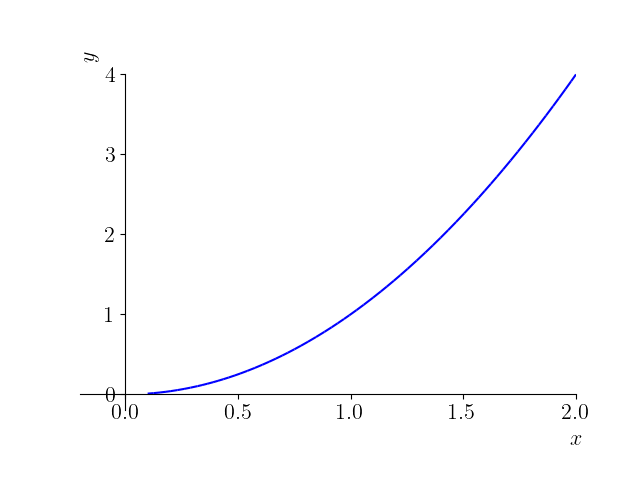
\includegraphics[width=0.7\textwidth]{./cap_funcao/dados/fig_cap_funcao_funabs/fig_cap_funcao_funabs}
  \caption{Esboço do gráfico da função valor absoluto $y=|x|$.}
  \label{fig:cap_funcao_funabs}
\end{figure}

\ifispython
Com o {\sympy}, a função valor absoluto é definida por \lstinline!abs()! ou \lstinline!Abs()!. Por exemplo, temos 
\begin{lstlisting}
  In : from sympy import *
  In : abs(-1)
  Out: 1
\end{lstlisting}
Use o {\sympy} para plotar o gráfico da função valor absoluto! Verifique com a Figura \ref{fig:cap_funcao_funabs}.
\fi

\subsection*{Exercícios}

\begin{flushright}
  [Vídeo] | [Áudio] | \href{https://phkonzen.github.io/notas/contato.html}{[Contatar]}
\end{flushright}

\begin{exer}
  Determine o domínio e a imagem da função identidade, i.e. $f(x) = x$. Então, faça o esboço de seu gráfico.
\end{exer}
\begin{resp}
  Domínio: $\mathbb{R}$; Imagem: $\mathbb{R}$
\end{resp}

\begin{exer}
  Determine o domínio e a imagem da função $f(x) = x^2 + 1$. Então, faça o esboço de seu gráfico.
\end{exer}
\begin{resp}
  Domínio: $\mathbb{R}$; Imagem: $[1, \infty)$.
\end{resp}

\begin{exer}
  Determine o domínio e a imagem da função $f(x) = 1 - x^2$. Então, faça o esboço de seu gráfico.
\end{exer}
\begin{resp}
  Domínio: $\mathbb{R}$; Imagem: $(-\infty, 1]$.
\end{resp}

\begin{exer}
  Determine o domínio e a imagem da função
  \begin{equation}
    h(x) = \frac{1}{x-1} - 2.
  \end{equation}
  Então, faça o esboço de seu gráfico.
\end{exer}
\begin{resp}
  Domínio: $(-\infty, 1)\cup (1, \infty)$; Imagem: $(-\infty, -2)\cup (-2, \infty)$.
\end{resp}

\begin{exer}
  Determine o domínio e a imagem da função valor absoluto.
\end{exer}
\begin{resp}
  Domínio: $\mathbb{R}$; Imagem: $[0, \infty)$.
\end{resp}

\section{Função Afim}\label{cap_funcao_sec_funafim}

\begin{flushright}
  [Vídeo] | [Áudio] | \href{https://phkonzen.github.io/notas/contato.html}{[Contatar]}
\end{flushright}

Uma \emph{função afim} é uma função da forma
\begin{equation}
f(x) = mx + b,
\end{equation}
sendo $m$ e $b$ parâmetros\footnote{números reais.} dados. O parâmetro $m$ é chamado de \pmb{coeficiente angular} e o parâmetro $b$ é chamado de \pmb{coeficiente constante}\footnote{Mais corretamente, coeficiente do termo constante.}.

Quando $m=0$, temos uma \emph{função constante} $f(x) = b$. Esta tem domínio $(-\infty, \infty)$ e imagem $\{b\}$. Quando $b=0$, temos uma \pmb{função linear} $f(x)=mx$, cujo domínio é $(-\infty, \infty)$ e imagem é $(-\infty, \infty)$.

De forma geral, toda função linear com $m\neq 0$ tem $(-\infty, \infty)$ como domínio e imagem.

\begin{ex}\label{ex:funafim}
  A Figura \ref{fig:ex_funafim} mostra esboços dos gráficos das funções afins $f(x)=-5/2$, $f(x)=2$ e $f(x)=2x-1$.
  
  \begin{figure}[H]
    \centering
    \includegraphics[width=0.7\textwidth]{./cap_funcao/dados/fig_ex_funafim/fig_ex_funafim}
    \caption{Esboços dos gráficos das funções afins $y=-5/2$, $y=2$ e $y=2x-1$ discutidas no Exemplo \ref{ex:funafim}.}
    \label{fig:ex_funafim}
  \end{figure}

  \ifispython
  Com o {\sympy}, podemos plotar o gráfico mostrado na Figura \ref{fig:ex_funafim} com o seguinte código:
  \begin{lstlisting}
    from sympy import *
    x = Symbol('x')
    p = plot(-5/2, (x,-2,2), line_color="blue", show=False)
    q = plot(2, (x,-2,2), line_color="red", show=False)
    p.extend(q)
    q = plot(2*x-1, (x,-2,2), line_color="green", show=False)
    p.extend(q)
    p[0].label = "$y=-5/2$"
    p[1].label = "$y=2$"
    p[2].label = "$y=$"
    p.legend = True
    p.show() 
  \end{lstlisting}
  \fi
\end{ex}

O lugar geométrico do gráfico de uma função afim é uma reta (ou linha). O coeficiente angular $m$ controla a \emph{inclinação da reta} em relação ao eixo $x$\footnote{eixo das abscissas}. Quando $m=0$, temos uma reta horizontal. Quando $m>0$ temos uma reta com inclinação positiva (crescente) e, quando $m<0$ temos uma reta com inclinação negativa.

\begin{ex}\label{ex:funlinear}
  A Figura \ref{fig:ex_funlinear} mostra esboços dos gráficos das funções lineares $f_1(x)=\frac{1}{2}x$, $f_2(x) = x$, $f_3(x) = 2x$, $f_4(x)=-2x$, $f_5(x)=-x$ e $f_6(x)=-\frac{1}{2}x$.
  
  \begin{figure}[H]
    \centering
    \includegraphics[width=0.7\textwidth]{./cap_funcao/dados/fig_ex_funlinear/fig_ex_funlinear}
    \caption{Esboços dos gráficos das funções lineares discutidas no Exemplo \ref{ex:funlinear}.}
    \label{fig:ex_funlinear}
  \end{figure}

  \ifispython
  Verifique, plotando os gráficos com o {\sympy}!
\end{ex}

\begin{figure}[H]
  \centering
  \includegraphics[width=0.7\textwidth]{./cap_funcao/dados/fig_declividade/fig_declividade}
  \caption{Declividade e o coeficiente angular.}
  \label{fig:declividade}
\end{figure}

A inclinação de uma reta é, normalmente, medida pelo \emph{ângulo de declividade} (veja a Figura \ref{fig:declividade}). Para definirmos este ângulo, sejam $(x_0, y_0)$ e $(x_1, y_1)$, $x_0<x_1$, pontos sobre uma dada reta, gráfico da função afim $f(x)=mx+b$. O ângulo de declividade (ou, simplesmente, a declividade) da reta é, por definição, o ângulo formado pelo segmento que parte de $(x_0, y_0)$ e termina em $(x_1, y_0)$ e o segmento que parte de $(x_0, y_0)$ e termina em $(x_1, y_1)$. Denotando este ângulo por $\theta$, temos
\begin{align}
  \tg\theta &= \frac{\text{cateto oposto}}{\text{cateto adjacente}}\\
            &= \frac{y_1-y_0}{x_1-x_0}\\
            &= \frac{mx_1+b-(mx_0+b)}{x_1-x_0}\\
            &= m,
\end{align}
o que justifica chamar $m$ de coeficiente angular.

Quaisquer dois pontos $(x_0, y_0)$ e $(x_1, y_1)$, com $x_0\neq x_1$, determinam uma única função afim (reta) que passa por estes pontos. Para encontrar a expressão desta função, basta resolver o seguinte sistema linear
\begin{align}
  mx_0 + b &= y_0\\
  mx_1 + b &= y_1
\end{align}
Subtraindo a primeira equação da segunda, obtemos
\begin{gather}
  m(x_0-x_1) = y_0-y_1\\
  m = \frac{y_0-y_1}{x_0-x_1}
\end{gather}
Daí, substituindo o valor de $m$ na primeira equação do sistema, obtemos
\begin{gather}
  \frac{y_0-y_1}{x_0-x_1}x_0 + b = y_0 \\
  b = -\frac{y_0-y_1}{x_0-x_1}x_0 + y_0
\end{gather}
Ou seja, a expressão da função linear (\emph{equação da reta}) que passa pelos pontos $(x_0, y_0)$ e $(x_1, y_1)$ é
\begin{equation}\label{eq:funafim_eq}
  y = \underbrace{\frac{y_0-y_1}{x_0-x_1}}_{m}(x-x_0) + y_0.
\end{equation}

\begin{ex}
  Vamos traçar o esboço da reta que representa o gráfico da função afim $f(x) = -x-1$. Para tanto, basta traçarmos a reta que passa por quaisquer dois pontos distintos de seu gráfico. Por exemplo, no caso da função $f(x) = -x -1$, temos
  \begin{center}
  \begin{tabular}[H]{r|c}
    $x$ & $y = -x-1$\\\hline
    -1  & 0\\
    1   & -2\\\hline
  \end{tabular}
\end{center}
Assim sendo, marcamos os pontos $(-1, 0)$ e $(1, -2)$ em um plano cartesiano e traçamos a reta que passa por eles. Veja a Figura \ref{fig:exeresol_funafim_grafico}.

\begin{figure}[H]
  \centering
  \includegraphics[width=0.7\textwidth]{./cap_funcao/dados/fig_exeresol_funafim_grafico/fig_exeresol_funafim_grafico}
  \caption{Esboço do gráfico da função afim $f(x)=-x-1$.}
  \label{fig:exeresol_funafim_grafico}
\end{figure}

\ifispython
Plote o gráfico com o {\sympy} e compare com o seu esboço!
\fi
\end{ex}

\begin{ex}
  Vamos determinar a função afim $f(x) = mx + b$, cujo gráfico contém os pontos $(1, -1)$ e $(2, 1)$. Para tanto, vamos usar \eqref{eq:funafim_eq}. Tomamos
  \begin{gather}
    (x_0, y_0) = (1, -1)\\
    (x_1, y_1) = (2, 1)
  \end{gather}
  Então, substituindo em \eqref{eq:funafim_eq} temos
  \begin{equation}
    m = \frac{y_1 - y_0}{x_1 - x_0} = \frac{1 - (-1)}{2 - 1} = 2.
  \end{equation}
  De \eqref{eq:funafim_eq}, temos
  \begin{align}
    f(x) &= m(x-x_0) + y_0\\
         &= 2(x - 1) + (-1) \\
         &= 2x -3.
  \end{align}
  Ou seja, a função afim desejada é $f(x) = 2x - 3$.

  \ifispython
  Com o {\sympy}, podemos resolver este exercício utilizando o seguinte código:
\begin{verbatim}
from sympy import *
x = Symbol('x')
x0 = 1
y0 = -1
x1 = 2
y1 = 1
m = (y1-y0)/(x1-x0)
f = Lambda(x, m*(x-x0) + y0)
print(f"f(x) = {f(x)}")
\end{verbatim}
  \fi
\end{ex}

\subsection*{Exercícios resolvidos}

\begin{exeresol}
  Faça o estudo de sinal da função
  \begin{equation}
    f(x) = 2x + 1
  \end{equation}
\end{exeresol}
\begin{resol}
  O estudo de sinal de uma função consiste em determinar as regiões de seu domínio em que seus valores de saída são negativos, zero ou positivos. Lembramos que uma função afim com coeficiente angular positivo é crescente em toda parte. Ainda, temos que ela corta o eixo das abscissas em sua raiz, i.e.
  \begin{gather}
    2x + 1 = 0\\
    2x = -1\\
    x = -\frac{1}{2}
  \end{gather}
  Por tanto, concluímos que
  \begin{center}
    \begin{tabular}{l|c|c|c}
      & $x<-\frac{1}{2}$ & $x=-\frac{1}{2}$ & $x>-\frac{1}{2}$\\\hline
      $f(x)$ & - & 0 & +  
    \end{tabular}
  \end{center}
  Ou seja, $f(x)$ é negativo para $x\in(-\infty,-\frac{1}{2})$, $f(x)=0$ para $x=-\frac{1}{2}$ e $f(x)$ é positivo para $x\in (-\frac{1}{2},\infty)$. Faça o esboço do gráfico de $f$ para verificar o resultado!
\end{resol}

\begin{exeresol}\label{exeresol:delim}
  Faça o esboço e hachure a região do plano cartesiano delimitada pelas retas $y=x+1$, $y=-3x+5$, $x=0$ e $x=2$.
\end{exeresol}
\begin{resol}
  A reta $y = 0$ corresponde ao eixo das ordenadas e $y=2$ é a reta perpendicular ao eixo das abscissas que passa pelo ponto $(2,0)$. Fazemos os esboços das retas em um único gráfico e então identificamos a região que está simultaneamente entre todas as retas dadas. Obtemos, assim, o gráfico abaixo.
  \begin{figure}[H]
    \centering
    \includegraphics[width=0.8\textwidth]{cap_funcao/dados/fig_exeresol_delim/fig}
    \caption{Gráfico da resolução do Exercício Resolvido \ref{exeresol:delim}.}
    \label{fig:exeresol_delim}
  \end{figure}
\end{resol}

\subsection*{Exercícios}

\begin{exer}
  Determine o domínio e a imagem de cada uma das seguintes funções afins:
  \begin{enumerate}[a)]
  \item $f(x) = -100x + 1$
  \item $y = -\pi$
  \item $h(v) = 2 + x$
  \end{enumerate}
\end{exer}
\begin{resp}
  a) $D=\mathbb{R}$; $I=\mathbb{R}$; b) $D=\mathbb{R}$, $I=\{\pi\}$; c) $D=\mathbb{R}$; $I=\mathbb{R}$
\end{resp}

\begin{exer}
  Faça um esboço do gráfico de cada uma das seguintes funções:
  \begin{enumerate}[a)]
  \item $f_1(x) = x$
  \item $f_2(x) = -x$
  \item $f_3(x) = x-1$
  \item $f_4(x) = -x+1$
  \end{enumerate}
\end{exer}

\begin{exer}
  Determine a função afim $f(x)=mx+b$, cujo gráfico contém os pontos $(-2, 1)$ e $(0, -2)$.
\end{exer}
\begin{resp}
  $f(x) = -\frac{3}{2}x - 2$
\end{resp}

\begin{exer}
  Faça o estudo de sinal das seguintes funções:
  \begin{enumerate}[a)]
  \item $f(x) = -2x - 2$
  \item $f(x) = -2$
  \item $f(x) = 2x - 2$
  \end{enumerate}
\end{exer}
\begin{resp}
  \begin{enumerate}[a)]
  \item
    \begin{tabular}{lccc}
      & $x<-1$ & $x=-1$ & $x>-1$\\
      $f(x)$ & + & 0 & -
    \end{tabular}
  \item $f(x)<0$ em toda parte
  \item 
    \begin{tabular}{lccc}
      & $x<1$ & $x=1$ & $x>1$\\
      $f(x)$ & - & 0 & +
    \end{tabular}
  \end{enumerate}
\end{resp}

\begin{exer}
  Verifique se as retas $y = -x - 1$ e $y = 2x - 3$ se interceptam e, caso afirmativo, determine o ponto de interseção.
\end{exer}
\begin{resp}
  $(2/3,-5/3)$
\end{resp}

\begin{exer}
  Determine o ponto de interseção dos gráficos das funções afins $f(x) = 2x + 1$ e $g(x) = 2x -1$.
\end{exer}
\begin{resp}
  não há
\end{resp}

\begin{exer}\label{exer:delim}
  Faça o esboço e hachure a região do plano cartesiano que fica delimitada pelas retas $y=0$, $y=2x+2$ e $x=1$.
\end{exer}

\begin{exer}(Aplicação.)
  Na \href{https://pt.wikipedia.org/wiki/Mec\%C3\%A2nica\_cl\%C3\%A1ssica}{mecânica clássica}, a \href{https://pt.wikipedia.org/wiki/Energia_cin\%C3\%A9tica}{energia cinética} $E_c$ de um objeto não rotativo de massa $m$ [$\text{kg}$] movimentando-se com uma velocidade $v$ [$\text{m}/\text{s}$] é dada por
  \begin{equation}
    E_c = \frac{m}{2}v^2
  \end{equation}
  Assumindo $v>0$ constante, temos que $E_c$ é função apenas de $m$, i.e. $E_c = E_c(m)$. Responda cada um dos seguintes itens:
  \begin{enumerate}[a)]
  \item Qual a classe da função $E_c = E_c(m)$?
  \item Qual o domínio da função $E_c = E_c(m)$.
  \item Qual a imagem da função $E_c = E_c(m)$.
  \item $E_c = E_c(m)$ é uma função crescente ou decresce?
  \item Se $E_c(1) = 50$, qual a velocidade do objeto?
  \end{enumerate}
\end{exer}
\begin{resp}
  a) Função linear. b) $D(E_v) = \{m\in \mathbb{R}:~m\geq 0\}$. c) $Im(E_v) = \{e\in \mathbb{R}: e\geq 0\}$. d) Sim. Valor mínimo $E_c=0$. Ponto de mínimo $v=0$. d) Crescente. e) $v=10$. 
\end{resp}


\section{Função Potência}\label{cap_funcao_sec_funpot}

\begin{flushright}
  [Vídeo] | [Áudio] | \href{https://phkonzen.github.io/notas/contato.html}{[Contatar]}
\end{flushright}

Uma função da forma $f(x)=x^n$, onde $n\neq 0$ é uma constante, é chamada de \emph{função potência}.

Funções potência têm comportamentos característicos conforme o valor de $n$. Quando $n$ é um inteiro positivo ímpar, seu domínio e sua imagem são $(-\infty, \infty)$. Veja a Figura \ref{fig:funpot_impar}.

\begin{figure}[H]
  \centering
  \includegraphics[width=0.7\textwidth]{./cap_funcao/dados/fig_funpot_impar/fig_funpot_impar}
  \caption{Esboços dos gráficos das funções potências $y=x$, $y=x^3$ e $y=x^5$.}
  \label{fig:funpot_impar}
\end{figure}

Funções potência com $n$ positivo par estão definidas em toda parte e têm imagem $[0, \infty)$. Veja a Figura \ref{fig:funpot_par}.

\begin{figure}[H]
  \centering
  \includegraphics[width=0.7\textwidth]{./cap_funcao/dados/fig_funpot_par/fig_funpot_par}
  \caption{Esboços dos gráficos das funções potências $y=x^2$, $y=x^4$ e $y=x^6$.}
  \label{fig:funpot_par}
\end{figure}

Funções potência com $n$ inteiro negativo ímpar não são definidas em $x=0$, tendo domínio e imagem igual a $(-\infty, 0)\cup (0, \infty)$. Também, quando $n$ inteiro negativo par, a função potência não está definida em $x=0$, tem domínio $(-\infty, 0)\cup (0, \infty)$, mas imagem $(0, \infty)$. Veja a Figura \ref{fig:funpot_negativo}.

\begin{figure}[H]
  \centering
  \includegraphics[width=0.5\textwidth]{./cap_funcao/dados/fig_funpot_negativo/fig_funpot_negativo_impar}~
    \includegraphics[width=0.5\textwidth]{./cap_funcao/dados/fig_funpot_negativo/fig_funpot_negativo_par}
  \caption{Esboços dos gráficos das funções potências $y=1/x$ (esquerda), $y=1/x^2$ (direita).}
  \label{fig:funpot_negativo}
\end{figure}

Há, ainda, comportamentos característicos quando $n=1/2$, $1/3$, $3/2$ e $2/3$. Veja a Figura \ref{fig:funpot_racional}.

\begin{figure}[H]
  \centering
  \includegraphics[width=0.5\textwidth]{./cap_funcao/dados/fig_funpot_racional/fig_funpot_racional_par}~
    \includegraphics[width=0.5\textwidth]{./cap_funcao/dados/fig_funpot_racional/fig_funpot_racional_impar}
  \caption{Esboços dos gráficos das funções potências. Esquerda $y=\sqrt{x}$ e $y=\sqrt{x^3}$. Direita: $y=\sqrt[3]{x}$ e $y=\sqrt[3]{x^2}$.}
  \label{fig:funpot_racional}
\end{figure}


\subsection*{Exercícios Resolvidos}

\begin{exeresol}\label{exeresol:funpot_graf}
  Determine o domínio e faça um esboço do gráfico de cada uma das seguintes funções:
  \begin{enumerate}[a)]
  \item $\displaystyle f(x) = x^{5/2}$;
  \item $\displaystyle g(x) = x^{5/3}$.
  \end{enumerate}
\end{exeresol}
\begin{resol}
  \begin{enumerate}[a)]
  \item Vamos analisar a função $f(x) = x^{5/2}$. Como $x^{5/2} = \sqrt{x^5}$ e não existe a raiz quadrada de número negativo, temos que $x^5$ deve ser não negativo. Daí, $x$ deve ser não negativo. Logo, o domínio de $f(x) = x^{5/2}$ é $[0, \infty)$. Veja o esboço desta função na Figura \ref{fig:exeresol_funpot_graf_a}.

    \begin{figure}[H]
      \centering
      \includegraphics[width=0.5\textwidth]{./cap_funcao/dados/fig_exeresol_funpot_graf/fig_exeresol_funpot_graf_a}
      \caption{Esboço do gráfico de $f(x) = x^{5/2}$.}
      \label{fig:exeresol_funpot_graf_a}
    \end{figure}

    \ifispython
    Verifique o gráfico plotando-o com o {\sympy}!
    \fi
  \item Vamos analisar a função $g(x) = x^{5/3}$. Como $x^{5/3} = \sqrt[3]{x^5}$, não temos restrição sobre os valores de $x$. Logo, o domínio da função $g$ é $(-\infty, \infty)$. Veja o esboço desta função na Figura \ref{fig:exeresol_funpot_graf_b}.
    
    \begin{figure}[H]
      \centering
      \includegraphics[width=0.5\textwidth]{./cap_funcao/dados/fig_exeresol_funpot_graf/fig_exeresol_funpot_graf_b}
      \caption{Esboço do gráfico de $g(x) = x^{5/3}$.}
      \label{fig:exeresol_funpot_graf_b}
    \end{figure}

    \ifispython
    Para plotar o gráfico de $g(x)$ com o {\sympy}, digitamos:
    \begin{lstlisting}
      from sympy import *
      p = plot(real_root(x**5,3),(x,-2,2))
    \end{lstlisting}
    \fi
  \end{enumerate}
\end{resol}

\begin{exeresol}\label{exeresol:funpot_intersep}
  Determine a equação da reta que passa pelos pontos de interseção dos gráficos das funções $f(x) = 1/x$ e $g(x) = \sqrt[3]{x}$.
\end{exeresol}
\begin{resol}
  Para determinarmos a reta precisamos, antes, dos pontos de interseção. As funções se interceptam nos pontos de abscissa $x$ tais que
  \begin{align}
    f(x) = g(x) &\Rightarrow \frac{1}{x} = \sqrt[3]{x}\\
                &\Rightarrow 1 = x\sqrt[3]{x}\\
                &\Rightarrow 1 = x\cdot x^{\frac{1}{3}}\\
                &\Rightarrow x^{1+\frac{1}{3}} = 1\\
                &\Rightarrow x^{\frac{4}{3}} = 1\\
                &\Rightarrow x^4 = \sqrt[3]{1}\\
                &\Rightarrow x^4 = 1\\
                &\Rightarrow x_0 = -1\quad\text{ou}\quad x_1=1.
  \end{align}
  Ou seja, os gráficos se interceptam nos pontos de abscissas $x_0 = -1$ e $x_1 = 1$. Veja o esboço dos gráficos das funções na Figura \ref{fig:exeresol_funpot_intersep}. Agora, podemos usar qualquer uma das funções para obter as ordenadas dos pontos de interseção. Usando $f(x)$, temos
  \begin{equation}
    (x_0, y_0) = (x_0, f(x_0)) = (-1, -1)
  \end{equation}
  e
  \begin{equation}
     (x_1, y_1) = (x_1, f(x_1)) = (1, 1)
  \end{equation}

  \begin{figure}[H]
    \centering
    \includegraphics[width=0.5\textwidth]{./cap_funcao/dados/fig_exeresol_funpot_intersep/fig_exeresol_funpot_intersep}
    \caption{Interseção dos gráficos das funções $f(x) = 1/x$ (azul) e $g(x) = \sqrt[3]{x}$ (vermelho).}
    \label{fig:exeresol_funpot_intersep}
  \end{figure}

  Agora, basta determinarmos a equação da reta que passa pelos pontos $(x_0, y_0) = (-1, -1)$ e $(x_1, y_1) = (1, 1)$. De \eqref{eq:funafim_eq}, temos que a equação da reta é tal que
  \begin{gather}
    y = \frac{y_1-y_0}{x_1-x_0}(x-x_0)+y_0 \\
    y = \frac{1-(-1)}{1-(-1)}(x-(-1))+(-1)\\
    y = x+1-1\\
    y = x.
  \end{gather}
  Ou seja, a que passa pelos pontos de interseção dos gráficos das funções $f(x)$ e $g(x)$ tem equação $y = x$.

  \ifispython
  Usando o {\sympy}, podemos resolver o problema com o seguinte código. 
  \begin{lstlisting}
    from sympy import *
    x = Symbol('x')
    f = Lambda(x, 1/x)
    g = Lambda(x, real_root(x,3))
    # x positivo
    x = Symbol('x', negative=True)
    x0 = solve(f(x)-g(x))[0]
    y0 = f(x0)
    # x negativo
    x = Symbol('x', positive=True)
    x1 = solve(f(x)-g(x))[0]
    y1 = f(x1)

    print(f"y = {(y1-y0)/(x1-x0)*(x-x0)+y0}")
  \end{lstlisting}
  \fi
\end{resol}

\subsection*{Exercícios}

\begin{flushright}
  [Vídeo] | [Áudio] | \href{https://phkonzen.github.io/notas/contato.html}{[Contatar]}
\end{flushright}

\begin{exer}
  Determine o domínio, a imagem e faça um esboço do gráfico de cada uma das seguintes funções:
  \begin{enumerate}[a)]
  \item $f(x) = x^7$;
  \item $g(x) = x^8$.
  \end{enumerate}
\end{exer}
\begin{resp}
  a) domínio: $(-\infty, \infty)$; imagem: $(-\infty, \infty)$. b) domínio: $(-\infty, \infty)$; imagem: $[0, \infty)$. Dica: use o \href{https://www.sympygamma.com/}{SymPy Gamma} para verificar os esboços de seus gráficos.
\end{resp}

\begin{exer}
  Determine o domínio, a imagem e faça um esboço do gráfico de cada uma das seguintes funções:
  \begin{enumerate}[a)]
  \item $\displaystyle f(x) = \frac{1}{x^7}$;
  \item $\displaystyle g(x) = \frac{1}{x^8}$.
  \end{enumerate}
\end{exer}
\begin{resp}
  a) domínio: $(-\infty, \infty)\setminus\{0\}$; imagem: $(-\infty, \infty)\setminus\{0\}$. b) domínio: $(-\infty, \infty)\setminus\{0\}$; imagem: $(0, \infty)$. Dica: use o \href{https://www.sympygamma.com/}{SymPy Gamma} para verificar os esboços de seus gráficos.
\end{resp}

\begin{exer}
  Determine o domínio, a imagem e faça um esboço do gráfico de cada uma das seguintes funções:
  \begin{enumerate}[a)]
  \item $\displaystyle f(x) = \sqrt{x^2}$;
  \item $\displaystyle g(x) = \sqrt[3]{x^3}$.
  \end{enumerate}
\end{exer}
\begin{resp}
  a) domínio: $(-\infty, \infty)$; imagem: $[0, \infty)$. b) domínio: $(-\infty, \infty)$; imagem: $(-\infty, \infty)$. Dica: use o \href{https://www.sympygamma.com/}{SymPy Gamma} para verificar os esboços de seus gráficos.
\end{resp}

\begin{exer}
  Determine o(s) ponto(s) de interseção entre as funções $f(x)=x$ e $g(x)=1/x$.
\end{exer}
\begin{resp}
  $(-1,-1)$, $(1,1)$
\end{resp}

\begin{exer}
  Determine a equação da reta que passa pelos pontos de interseção entre as funções $f(x)=x^2$ e $g(x)=1/x^2$.
\end{exer}
\begin{resp}
  $y=1$
\end{resp}


\section{Função Polinomial}\label{cap_funcao_sec_funpoli}

\begin{flushright}
  [Vídeo] | [Áudio] | \href{https://phkonzen.github.io/notas/contato.html}{[Contatar]}
\end{flushright}

Uma \emph{função polinomial} (\emph{polinômio}) tem a forma
\begin{equation}
  p(x) = a_nx^n + a_{n-1}x^{n-1} + \cdots + a_1x + a_0,
\end{equation}
onde $a_i$ são coeficientes reais, $a_n\neq 0$ e $n$ é inteiro não negativo, este chamado de \emph{grau do polinômio}.

Polinômios são definidos em toda parte\footnote{Uma função é dita ser definida em toda parte quando seu domínio é $(\infty, \infty)$}. Polinômios de grau ímpar tem imagem $(-\infty, \infty)$. Entretanto, a imagem polinômios de grau par dependem de cada caso. Iremos estudar mais propriedades de polinômios ao longo do curso de cálculo. Veja a Figura \ref{fig:poli_graficos}.

\begin{figure}[H]
  \centering
  \includegraphics[width=0.5\textwidth]{./cap_funcao/dados/fig_poli_graficos/fig_poli_impar}~
    \includegraphics[width=0.5\textwidth]{./cap_funcao/dados/fig_poli_graficos/fig_poli_par}
  \caption{Esboços dos gráficos das funções polinomiais. Esquerda: $p(x) = x^{3} - 2.5 x^{2} - 1.0 x + 2.5$. Direita: $q(x) = x^{4} - 3.5 x^{3} + 1.5 x^{2} + 3.5 x - 2.5$.}
  \label{fig:poli_graficos}
\end{figure}

Quando $n=0$, temos um polinômio de grau 0 (ou uma função constante). Quando $n=1$, temos um polinômio de grau 1 (ou, uma função afim). Ainda, quando $n=2$ temos uma \emph{função quadrática} (ou \emph{polinômio quadrático}) e, quando $n=3$, temos uma \emph{função cúbica} (ou \emph{polinômio cúbico}).

\subsection{Função Quadrática}

\begin{flushright}
  [Vídeo] | [Áudio] | \href{https://phkonzen.github.io/notas/contato.html}{[Contatar]}
\end{flushright}

Os polinômios de grau 2 são, também, chamados de \emph{funções quadráticas}, i.e. funções da forma
\begin{equation}
  f(x) = ax^2 + bx + c,
\end{equation}
onde $a$ é chamado de \emph{coeficiente do termo quadrático}, $b$ o \emph{coeficiente do termo linear} e $c$ o \emph{coeficiente do termo constante}.

Os zeros de uma função quadrática podem ser calculados pela \emph{fórmula de Bhaskara}
\begin{equation}\label{eq:Bhaskara}
  x_0, x_1 = \frac{-b \pm \sqrt{b^2 - 4ac}}{2a}.
\end{equation}

O esboço do gráfico de uma função quadrática é uma \emph{parábola côncava para cima} quando $a > 0$ e, \emph{côncava para baixo} quando $x < 0$. Veja a Figura \ref{fig:funquad_concavidade}.

\begin{figure}[H]
  \centering
  \includegraphics[width=0.5\textwidth]{./cap_funcao/dados/fig_funquad_concavidade/fig_funquad_concavidade_cima}~
    \includegraphics[width=0.5\textwidth]{./cap_funcao/dados/fig_funquad_concavidade/fig_funquad_concavidade_baixo}
  \caption{Esboço dos gráficos das funções quadráticas: $f(x) = x^2-x-2$ (esquerda) e $g(x)=-x^2+x+2$ (direita).}
  \label{fig:funquad_concavidade}
\end{figure}

O \emph{vértice} da parábola que representa uma função quadrática $f(x)$ com coeficiente quadrático positivo (com coeficiente quadrático negativo) é o ponto no qual ela atinge seu \emph{valor mínimo (máximo)} em todo o seu domínio natural. Quando $f$ têm zeros reais, o ponto de abscissa do vértice é o ponto médio entre os zeros $x_0$ e $x_1$ da função, i.e. o vértice $V = (x_v, y_v)$ é tal que
\begin{equation}
  x_v = \frac{x_0 + x_1}{2},\quad\text{e}\quad y_v = f(x_v). 
\end{equation}
O valor $x_v$ é a abscissa do ponto em que a função quadrática $f$ atinge o \emph{valor máximo (valor mínimo)} $y_v$. Em geral, o vértice é dado por
\begin{equation}
  (x_v,y_v) = \left(-\frac{b}{2a},-\frac{b^2-4ac}{4a}\right)
\end{equation}

\subsection*{Exercícios Resolvidos}

\begin{exeresol}
  Determine os zeros do polinômio $f(x) = x^3-x^2-2x$.
\end{exeresol}
\begin{resol}
  Determinar os zeros da função $f$ significa encontrar todos os valores de $x$ tais que $f(x)=0$ (estes são as abscissas dos pontos nos quais o gráfico de $f$ intercepta o eixo das abscissas). Temos
  \begin{gather}
    f(x)=0\\
    x^3-x^2-2x=0\\
    x(x^2-x-2)=0\\
    x=0\quad\text{ou}\quad x^2-x-2=0.
  \end{gather}
  Então, usando a fórmula de Bhaskara \eqref{eq:Bhaskara} na equação $x^2-x-2=0$, obtemos
  \begin{align}
    x &= \frac{-b\pm\sqrt{b^2-4ac}}{2a} \\
      &= \frac{1\pm\sqrt{1-4\cdot 1\cdot (-2)}}{2}\\
      &= \frac{1\pm\sqrt{9}}{2}\\
      &= \frac{1\pm 3}{2}\\
      &= -1\quad\text{ou}\quad 2
  \end{align}
  Com isso, temos que os zeros da função $f$ ocorrem nos pontos $x_0 = -1$, $x_1=0$ e $x_2=2$.

  \ifispython
  Com o {\sympy}, podemos calcular os zeros da função $f$ com o seguinte comando:
  \begin{lstlisting}
    from sympy import *
    solve(x**3-x**2-2*x)
  \end{lstlisting}
  \fi
\end{resol}

\begin{exeresol}
  Determine o valor mínimo da função $f(x) = x^2 - x - 2$.
\end{exeresol}
\begin{resol}
  Como $f$ é uma função quadrática com coeficiente quadrático positivo, temos que seu gráfico é uma parábola côncava para cima. Logo, $f$ atinge seu valor mínimo no seu vértice, que tem abscissa
  \begin{align}
    x_v &= -\frac{b}{2a}\\
        &= -\frac{-1}{2\cdot 1}\\
        &= \frac{1}{2}.
  \end{align}
  Ou seja, a abscissa do ponto de mínimo de $f$ é $x_v=1/2$ e seu valor mínimo é
  \begin{align}
    f\left(\frac{1}{2}\right) &= \left(\frac{1}{2}\right)^2-\frac{1}{2}-2\\
                              &= \frac{1-2-8}{4}\\
                              &= -\frac{9}{4}.
  \end{align}

  \ifispython
  Usando {\sympy}, podemos resolver este exercício com o seguinte código:
  \begin{lstlisting}
    from sympy import *
    x = Symbol('x')
    a = 1
    b = -1
    c = -2
    f = Lambda(x, a*x**2 + b*x + c)
    xv = -b/(2*a)
    print(f"Valor mínimo = {f(xv)}")
  \end{lstlisting}
  \fi
\end{resol}

\subsection*{Exercícios}

\begin{flushright}
  [Vídeo] | [Áudio] | \href{https://phkonzen.github.io/notas/contato.html}{[Contatar]}
\end{flushright}

\begin{exer}
  Faça o esboço dos gráficos das seguintes funções polinomiais:
  \begin{enumerate}
  \item $f(x) = 1$
  \item $g(x) = -x + 1$
  \item $h(x) = x^2 - 1$
  \item $f_1(x) = x^3$
  \end{enumerate}
\end{exer}

\begin{exer}
  Determine os zeros do polinômio $f(x) = -x^3+x^2+2x$.
\end{exer}
\begin{resp}
  $-1$, $0$, $2$
\end{resp}

\begin{exer}
  Determine o valor máximo da função $f(x) = -x^2 + x + 2$.
\end{exer}
\begin{resp}
  $9/4$
\end{resp}

\begin{exer}
  Faça um esboço da região determinada entre os gráficos de $y=0$ e $y=x^2-1$, com $-1\leq x \leq 1$.
\end{exer}

\begin{exer}
  Determine os pontos de interseção dos gráficos de $f(x)=-x+1$ e $f(x)=x^2-1$. 
\end{exer}
\begin{resp}
  $(-2,3)$, $(1,0)$
\end{resp}

\begin{exer}(Aplicação.)
  Na \href{https://pt.wikipedia.org/wiki/Mec\%C3\%A2nica\_cl\%C3\%A1ssica}{mecânica clássica}, a \href{https://pt.wikipedia.org/wiki/Energia_cin\%C3\%A9tica}{energia cinética} $E_c$ de um objeto não rotativo de massa $m$ [$\text{kg}$] movimentando-se com uma velocidade $v$ [$\text{m}/\text{s}$] é dada por
  \begin{equation}
    E_c = \frac{m}{2}v^2
  \end{equation}
  Assumindo $m>0$ constante, temos que $E_c$ é função apenas de $v$, i.e. $E_c = E_c(v)$. Responda cada um dos seguintes itens:
  \begin{enumerate}[a)]
  \item Qual a classe da função $E_c = E_c(v)$?
  \item Qual o domínio da função $E_c = E_c(v)$.
  \item Qual a imagem da função $E_c = E_c(v)$.
  \item A função $E_c=E_c(v)$ tem valor mínimo? Se sim, qual é esse valor e para o valor de $v$ em que isso ocorre?
  \end{enumerate}
\end{exer}
\begin{resp}
  a) função quadrática. b) $D(E_v) = \{v\in \mathbb{R}:~-c\leq v\leq c\}$, onde $c$ denota a \href{https://pt.wikipedia.org/wiki/Velocidade\_da\_luz}{velocidade da luz}. c) $Im(E_v) = \{e\in \mathbb{R}: 0\leq e\leq \frac{m\cdot c^2}{2}\}$, onde $c$ denota a \href{https://pt.wikipedia.org/wiki/Velocidade\_da\_luz}{velocidade da luz}. d) Sim. Valor mínimo $E_c=0$. Ponto de mínimo $v=0$.
\end{resp}

\section{Função Racional}\label{cap_funcao_sec_funracio}

\begin{flushright}
  [Vídeo] | [Áudio] | \href{https://phkonzen.github.io/notas/contato.html}{[Contatar]}
\end{flushright}

Uma \emph{função racional} tem a forma
\begin{equation}
  f(x) = \frac{p(x)}{q(x)},
\end{equation}
onde $p(x)$ e $q(x)\not\equiv 0$ são polinômios.

Funções racionais não estão definidas nos zeros de $q(x)$. Além disso, suas imagens dependem de cada caso. Estudaremos o comportamento de funções racionais ao longo do curso de cálculo. Como exemplo, veja a Figura \ref{fig:racional_grafico} para um esboço do gráfico da função racional
\begin{equation}
  f(x) = \frac{x^2-x-2}{x^3-x^2+x-1}.
\end{equation}

\begin{figure}[H]
  \centering
  \includegraphics[width=0.8\textwidth]{./cap_funcao/dados/fig_racional_grafico/fig_racional_grafico}
  \caption{Esboço do gráfico da função racional $\displaystyle f(x) = \frac{x^{2} - x - 2}{x^{3} - x^{2} + x - 1}$.}
  \label{fig:racional_grafico}
\end{figure}

Com o estudo do \emph{cálculo de limites}, veremos que a reta $y = 0$ (eixo das abscissas) é uma \emph{assíntota horizontal} e a reta $x=1$ (reta tracejada) é uma \emph{assíntota vertical} ao gráfico desta função. Esta singularidade no ponto $x=1$ está relacionada ao fato de que o denominador se anula em $x=1$. Ainda, para $x\neq 1$ temos
\begin{equation}
  \frac{x^3 - x^2 + x - 1}{x-1} = x^2 + 1,
\end{equation}
Com isso, podemos concluir que o domínio da função $f(x)$ é $\mathbb{R}\setminus\{0\}$.


\subsection*{Exercícios Resolvidos}

\begin{flushright}
  [Vídeo] | [Áudio] | \href{https://phkonzen.github.io/notas/contato.html}{[Contatar]}
\end{flushright}

\begin{exeresol}
  Determine o domínio da função racional
  \begin{equation}
    f(x) = \frac{x^3-x^2+x-1}{x^2-1}.
  \end{equation}
\end{exeresol}
\begin{resol}
  Como $f(x)$ é uma função racional, ela não está definida nos zeros do polinômio que constitui seu denominador. I.e., nos pontos
  \begin{equation}
    x^2-1=0\Rightarrow x = \pm 1.
  \end{equation}
  Logo, o domínio de $f(x)$ é o conjunto $\mathbb{R}\setminus\{-1, 1\}$.
\end{resol}

\begin{exeresol}
  Determine o domínio e faça o esboço do gráfico da função racional
  \begin{equation}
    g(x) = \frac{x-1}{x-1}.
  \end{equation}
\end{exeresol}
\begin{resol}
  Tendo em vista que o denominador se anula em $x=1$, o domínio de $g$ é $(-\infty, 0)\cup (0, \infty)$. Agora, para fazermos um esboço de seu gráfico, observamos que $g(x)=1$ para $x\neq 1$. I.e., $g$ é uma função constante para valores de $x\neq 1$ e não está definida em $x=1$. Veja a Figura \ref{fig:exeresol_funracio_graf} para o esboço do gráfico da função $g$.

  \begin{figure}[H]
    \centering
    \includegraphics[width=0.8\textwidth]{./cap_funcao/dados/fig_exeresol_funracio_graf/fig_exeresol_funracio_graf}
    \caption{Esboço do gráfico da função $g(x) = (x-1)/(x-1)$.}
    \label{fig:exeresol_funracio_graf}
  \end{figure}

  \ifispython
  Usando o {\sympy}, os comandos
  \begin{lstlisting}
    from sympy import *
    plot((x-1)/(x-1),(x,-2,2))
  \end{lstlisting}
  plota uma linha constante, sem identificar a singularidade em $x=1$. Isto ocorre, pois os gráficos com o {\sympy} são obtidos a partir de uma amostra discreta de pontos. Ocorre que esta amostra pode não conter as singularidades. No caso de conter, a execução pode não plotar o gráfico e retornar um erro.

  Devemos ficar atentos a esboços de gráficos obtidos no computador, muitas vezes os gráficos podem estar errados. Cabe ao usuário identificar e analisar pontos e região de interesse.
  \fi
\end{resol}

\subsection*{Exercícios}

\begin{flushright}
  [Vídeo] | [Áudio] | \href{https://phkonzen.github.io/notas/contato.html}{[Contatar]}
\end{flushright}

\begin{exer}
  Determine o domínio e faça um esboço do gráfico da função racional
  \begin{equation}
    y = \frac{1}{x-1}
  \end{equation}
\end{exer}
\begin{resp}
  $D=\mathbb{R}\setminus\{1\}$
\end{resp}

\begin{exer}
  Determine o domínio da função racional
  \begin{equation}
    f(x) = \frac{x^2+1}{x^2-5x+6}
  \end{equation}
\end{exer}
\begin{resp}
  $D=\mathbb{R}\setminus\{2,3\}$
\end{resp}

\begin{exer}
  Determine o domínio e faça o esboço do gráfico da função racional
  \begin{equation}
    f(x) = \frac{x^2-1}{x^3-x}.
  \end{equation}
\end{exer}
\begin{resp}
  $\mathbb{R}\setminus\{-1,0,1\}$
\end{resp}

\begin{exer}
  Encontre o(s) ponto(s) de interseção entre os gráficos das funções
  \begin{equation}
    f(x) = \frac{1}{x-1}
  \end{equation}
  e
  \begin{equation}
    g(x) = \frac{x^2-1}{x-x^3}
  \end{equation}
\end{exer}
\begin{resp}
  $x=\frac{1}{2}$
\end{resp}

\begin{exer}
  Determine os zeros da função racional
  \begin{equation}
    f(x) = \frac{x^2-1}{x^2-5x+6}
  \end{equation}
\end{exer}
\begin{resp}
  $\{-1,1\}$
\end{resp}

\begin{exer}(Aplicação.)
  A \href{https://pt.wikipedia.org/wiki/Lei\_de\_Boyle-Mariotte}{Lei de Boyle-Mariotte} enuncia que são inversamente proporcionais a pressão $P$ e o volume $V$ de um gás ideal confinado e mantido a uma temperatura constante. Responda cada um dos seguintes itens:
  \begin{enumerate}[a)]
  \item Escreva $P$ como função de $V$.
  \item Classifique a função $P = P(V)$.
  \item Determine o domínio da função $P = P(V)$.
  \item Determine a imagem da função $P = P(V)$.
  \item Faça um esboço do gráfico da função $P = P(V)$.
  \end{enumerate}
\end{exer}
\begin{resp}
  a) $\displaystyle P = \alpha\cdot V$, para algum parâmetro $\alpha>0$. b) Função racional. c) $D(P) = \{v\in\mathbb{R}:~v>0\}$. d) $Im(P) = \{p\in\mathbb{R}:~p>0\}$. 
\end{resp}


\section{Funções Trigonométricas}\label{cap_funcao_sec_funtri}

\begin{flushright}
  [Vídeo] | [Áudio] | \href{https://phkonzen.github.io/notas/contato.html}{[Contatar]}
\end{flushright}

Funções trigonométricas são funções transcendentes e são construídas a partir do estudo trigonométrico de triângulos retângulos.

\subsection{Seno e Cosseno}

\begin{flushright}
  [Vídeo] | [Áudio] | \href{https://phkonzen.github.io/notas/contato.html}{[Contatar]}
\end{flushright}

As funções trigonométricas seno $y=\sen(x)$ e cosseno $y=\cos(x)$ podem ser definidas a partir do \emph{círculo trigonométrico} (veja a Figura \ref{fig:cos_seno}). Seja $x$ o ângulo\footnote{Em geral utilizaremos a medida em radianos para ângulos.} de declividade da reta que passa pela origem do plano cartesiano (reta $r$ na Figura \ref{fig:cos_seno}). Seja, então, $(a,b)$ o ponto de interseção desta reta com a circunferência unitária\footnote{Circunferência do círculo de raio 1.}. Então, definimos:
\begin{equation}
  \sen(x) = b,\qquad \cos(x) = a.
\end{equation}
A partir da definição, notamos que ambas funções têm domínio $(-\infty, \infty)$ e imagem $[-1, 1]$.

\begin{figure}[H]
  \centering
  \includegraphics[width=0.8\textwidth]{./cap_funcao/dados/fig_cos_seno/fig_cos_seno}
  \caption{Funções seno e cosseno no círculo trigonométrico.}
  \label{fig:cos_seno}
\end{figure}

Na Figura \ref{fig:cos_seno_valores} podemos extrair os valores das funções seno e cosseno para os ângulos fundamentais. Por exemplo, temos
\begin{align}
  &\sen\left(\frac{\pi}{6}\right) = \frac{1}{2},\qquad \cos\left(\frac{\pi}{6}\right) = \frac{\sqrt{3}}{2},\\
  &\sen\left(\frac{3\pi}{4}\right) = \frac{\sqrt{2}}{2},\qquad \cos\left(\frac{\pi}{4}\right) = -\frac{\sqrt{2}}{2},\\
  &\sen\left(\frac{8\pi}{6}\right) = -\frac{\sqrt{3}}{2},\qquad \cos\left(\frac{8\pi}{6}\right) = -\frac{1}{2},\\
  &\sen\left(\frac{11\pi}{6}\right) = -\frac{1}{2},\qquad \cos\left(\frac{11\pi}{6}\right) = \frac{\sqrt{3}}{2},\\
\end{align}
\ifispython
As funções seno e cosseno estão definidas no {\sympy} como \verb+sin+ e $\verb+cos+$, respectivamente. Por exemplo, para computar o seno de $\pi/6$, digitamos:
\begin{lstlisting}
  from sympy import *
  sin(pi/6)
\end{lstlisting}
\fi

\begin{figure}[H]
  \centering
  \includegraphics[width=1\textwidth]{./cap_funcao/dados/fig_cos_seno_valores/fig_cos_seno_valores}
  \caption{Funções seno e cosseno no círculo trigonométrico.}
  \label{fig:cos_seno_valores}
\end{figure}

Uma \emph{função} $f(x)$ é dita \emph{periódica} quando existe um número $p$, chamado de \emph{período} da função, tal que
\begin{equation}
  f(x+p) = f(x)
\end{equation}
para qualquer valor de $x$ no domínio da função. Da definição das funções seno e cosseno, observamos que ambas são periódicas com período $2\pi$, i.e.
\begin{equation}
  \sen(x+2\pi) = \sen(x)
\end{equation}
e
\begin{equation}
   \cos(x+2\pi) = \cos(x)
\end{equation}
para qualquer valor de $x$.

A Figura \ref{fig:seno} contém o esboço do gráfico da função seno e a Figura \ref{fig:cos} o da função cosseno.

\begin{figure}[H]
  \centering
  \includegraphics[width=0.8\textwidth]{./cap_funcao/dados/fig_cos_seno_graficos/fig_seno_grafico}
  \caption{Esboço do gráfico de $y=\sen x$.}
  \label{fig:seno}
\end{figure}

\begin{figure}[H]
  \centering
  \includegraphics[width=0.8\textwidth]{./cap_funcao/dados/fig_cos_seno_graficos/fig_cosseno_grafico}
  \caption{Esboço do gráfico de $y=\cos x$.}
  \label{fig:cos}
\end{figure}


\subsection{Tangente, Cotangente, Secante e Cossecante}

\begin{flushright}
  [Vídeo] | [Áudio] | \href{https://phkonzen.github.io/notas/contato.html}{[Contatar]}
\end{flushright}

Das funções seno e cosseno, definimos as funções \emph{tangente}, \emph{cotangente}, \emph{secante} e \emph{cossecante} como seguem:
\begin{gather}
  \tg(x) := \frac{\sen(x)}{\cos(x)}\\
  \cotg(x) := \frac{\cos(x)}{\sen(x)}\\
  \sec(x) := \frac{1}{\cos(x)},\\
  \cosec(x) := \frac{1}{\sen(x)}
\end{gather}

\ifispython
No {\python}+{\sympy}, as funções tangente, cotangente, secante e cossecante podem ser computadas com as funções $\verb+tan+$, $\verb+cot+$, $\verb+sec+$ e $\verb+csc+$, respectivamente. Por exemplo, podemos computar o valor de $\cosec(\pi/4)$ com o comando
\begin{lstlisting}
In : from sympy import *
...: csc(pi/4)
Out: sqrt(2)
\end{lstlisting}
\fi

Na Figura \ref{fig:tg_grafico}, temos o esboço do gráfico da função \emph{tangente} e na Figura \ref{fig:cotg_grafico} o da \emph{cotangente}. Observemos que a função tangente não está definida nos pontos $(2k+1)\pi/2$, para todo $k$ inteiro. Já, a função cotangente não está definida nos pontos $k\pi$, para todo $k$ inteiro. Ambas estas funções têm imagem $(-\infty, \infty)$ e período $\pi$.

\begin{figure}[H]
  \centering
  \includegraphics[width=0.8\textwidth]{./cap_funcao/dados/fig_co_tg_graficos/fig_tg_grafico}\\
  \caption{Esboço do gráfico de $y=\tg x$.}
  \label{fig:tg_grafico}
\end{figure}

\begin{figure}[H]
  \centering
  \includegraphics[width=0.8\textwidth]{./cap_funcao/dados/fig_co_tg_graficos/fig_cotg_grafico}
  \caption{Esboço do gráfico de $y=\cotg x$.}
  \label{fig:cotg_grafico}
\end{figure}

Na Figura \ref{fig:sec_grafico}, temos o esboço do gráfico da função \emph{secante} e na Figura \ref{fig:cossec_grafico} o da função \emph{cossecante}. Observemos que a função secante não está definida nos pontos $(2k+1)\pi/2$, para todo $k$ inteiro. Já, a função cossecante não está definida nos pontos $k\pi$, para todo $k$ inteiro. Ambas estas funções têm imagem $(-\infty, 1]\cup [1, \infty)$ e período $\pi$.

\begin{figure}[H]
  \centering
  \includegraphics[width=0.8\textwidth]{./cap_funcao/dados/fig_co_sec_graficos/fig_sec_grafico}
  \caption{Esboço do gráfico da função secante.}
  \label{fig:sec_grafico}
\end{figure}

\begin{figure}[H]
  \centering
  \includegraphics[width=0.8\textwidth]{./cap_funcao/dados/fig_co_sec_graficos/fig_cosec_grafico}
  \caption{Esboço do gráfico da função cossecante.}
  \label{fig:cossec_grafico}
\end{figure}

\subsection{Identidades Trigonométricas}

\begin{flushright}
  [Vídeo] | [Áudio] | \href{https://phkonzen.github.io/notas/contato.html}{[Contatar]}
\end{flushright}

Aqui, vamos apresentar algumas identidades trigonométricas que serão utilizadas ao longo do curso de cálculo. Comecemos pela \emph{identidade fundamental}
\begin{equation}
  \sen^2 x + \cos^2 x = 1.
\end{equation}
Desta decorrem as identidades
\begin{align}
  &\tg^2(x) + 1 = \sec^2 x,\\
  &1 + \cotg^2(x) = \cosec^2(x).
\end{align}

Das seguintes fórmulas para adição/subtração de ângulos
\begin{align}
  &\cos(x\pm y) = \cos(x)\cos(y) \mp \sen(x)\sen(y),\\
  &\sen(x\pm y) = \sen(x)cos(y) \pm \cos(x)\sen(y),
\end{align}
seguem as fórmulas para ângulo duplo
\begin{align}
  &\cos(2x) = \cos^2x - \sen^2x,\\
  &\sen(2x) = 2\sen x\cos x.
\end{align}

Também, temos as fórmulas para o ângulo metade
\begin{align}
  &\cos^2 x = \frac{1 + \cos 2x}{2},\\
  &\sen^2 x = \frac{1 - \cos 2x}{2}.\label{eq:id_trig_cos_x2}
\end{align}

\subsection*{Exercícios Resolvidos}

\begin{flushright}
  [Vídeo] | [Áudio] | \href{https://phkonzen.github.io/notas/contato.html}{[Contatar]}
\end{flushright}

\begin{exeresol}
  Mostre que
  \begin{equation}
    \cos x - 1 = -2\sen^2 \frac{x}{2}.
  \end{equation}
\end{exeresol}
\begin{resol}
  A identidade trigonométrica
  \begin{equation}
    \sen^2 x = \frac{1 - \cos 2x}{2},
  \end{equation}
  aplicada a metade do ângulo, fornece
  \begin{equation}
    \sen^2 \frac{x}{2} = \frac{1 - \cos x}{2}.
  \end{equation}
  Então, isolando $\cos x$, obtemos
  \begin{gather}
    \sen^2 \frac{x}{2} = \frac{1 - \cos x}{2}\\
    1 - \cos x = 2\sen^2 \frac{x}{2}\\
    \cos x - 1 = -2\sen^2 \frac{x}{2}.
  \end{gather}
\end{resol}

\subsection*{Exercícios}

\begin{flushright}
  [Vídeo] | [Áudio] | \href{https://phkonzen.github.io/notas/contato.html}{[Contatar]}
\end{flushright}

\begin{exer}
  Calcule os seguintes valores
  \begin{enumerate}[a)]
  \item $\sen(7\pi/6)$
  \item $\cos(7\pi/6)$
  \item $\tg(7\pi/6)$
  \item $\cotg(7\pi/6)$
  \item $\sec(7\pi/6)$
  \item $\cosec(7\pi/6)$
  \end{enumerate}
\end{exer}
\begin{resp}
  a) $-1/2$; b) $-\sqrt{3}/2$; c) $\sqrt{3}/3$; d) $\sqrt{3}$; e) $-2\sqrt{3}/3$; f) $-2$
\end{resp}

\begin{exer}
  Calcule os seguintes valores
  \begin{enumerate}[a)]
  \item $\sen(-pi/3)$
  \item $tg(-3\pi/4)$
  \item $\cos(19\pi/6)$
  \end{enumerate}
\end{exer}
\begin{resp}
  a) $-\sqrt{3}/2$; b) $1$; c) $-\sqrt{3}/2$
\end{resp}

\begin{exer}
  Mostre que $\sen x$ é  uma \emph{função ímpar}\footnote{Por definição, $f(x)$ é função ímpar quando $f(x)=-f(-x)$.}, i.e.
  \begin{equation}
    \sen x = -\sen(-x)
  \end{equation}
  para todo número real $x$.
\end{exer}
\begin{resp}
  Dica: analise o ciclo trigonométrico.
\end{resp}

\begin{exer}
  Mostre que $\cos x$ é  uma \emph{função par}\footnote{Por definição, $f(x)$ é uma função par quando $f(x)=f(-x)$.}, i.e.
  \begin{equation}
    \cos x = \cos(-x)
  \end{equation}
  para todo número real $x$.
\end{exer}
\begin{resp}
  Dica: analise o ciclo trigonométrico.
\end{resp}

\begin{exer}
  Determine os pontos de interseção entre as funções $f(x)=2x/\pi$ e $g(x)=\sen(x)$.
\end{exer}
\begin{resp}
  $(-\pi/2, -1)$, $(0,0)$, $(\pi/2, 1)$
\end{resp}

\section{Operações com Funções}\label{cap_funcao_sec_opfun}

\begin{flushright}
  [Vídeo] | [Áudio] | \href{https://phkonzen.github.io/notas/contato.html}{[Contatar]}
\end{flushright}

\subsection{Soma , Diferença , Produto  e Quociente }

\begin{flushright}
  [Vídeo] | [Áudio] | \href{https://phkonzen.github.io/notas/contato.html}{[Contatar]}
\end{flushright}

Sejam dadas as funções $f$ e $g$ com domínio em comum $D$. Então, definimos as funções
\begin{itemize}
\item $(f\pm g)(x) := f(x) \pm g(x)$ para todo $x\in D$;
\item $(f\cdot g)(x) := f(x)\cdot g(x)$ para todo $x\in D$;
\item $\displaystyle \left(\frac{f}{g}\right)(x) := \frac{f(x)}{g(x)}$ para todo $x\in D$ tal que $g(x)\neq 0$.
\end{itemize}

\begin{ex}
  Sejam $f(x)=x^2$ e $g(x)=x$. Temos:
  \begin{enumerate}[a)]
  \item $(f+g)(x) = x^2 + x$ e está definida em toda parte.
  \item $(g-f)(x) = x - x^2$ e está definida em toda parte.
  \item $(f\cdot g)(x) = x^3$ e está definida em toda parte.
  \item $\displaystyle \left(\frac{f}{g}\right)(x) = \frac{x^2}{x}$ e tem domínio $\mathbb{R}\setminus \{0\}$\footnote{Observemos que não podemos simplificar o $x$, pois a função $y=x$ é diferente da função $y=x^2/x$.}.
  \end{enumerate}
\end{ex}

\subsection{Função Composta}

\begin{flushright}
  [Vídeo] | [Áudio] | \href{https://phkonzen.github.io/notas/contato.html}{[Contatar]}
\end{flushright}

Sejam dadas as funções $f$ e $g$. Definimos a \emph{função composta} de $f$ com $g$ por
\begin{equation}
  (f\circ g)(x) := f\left(g(x)\right).
\end{equation}
Seu domínio consiste dos valores de $x$ que pertençam ao domínio da $g$ e tal que $g(x)$ pertença ao domínio da $f$. Em notação matemática
\begin{equation}
  D_{f\circ g} = \{x\in D_g:~g(x)\in D_f\}
\end{equation}

\begin{ex}
  Sejam $f(x) = x^2$ e $g(x) = x+1$. A função composta de $f$ com $g$ é
  \begin{align}
    (f\circ g)(x) &= f\left(g(x)\right)\\
                  &= f(x+1) = (x+1)^2
  \end{align}
\end{ex}

\subsection{Translação, Contração, Dilatação e Reflexão de Gráficos}

\begin{flushright}
  [Vídeo] | [Áudio] | \href{https://phkonzen.github.io/notas/contato.html}{[Contatar]}
\end{flushright}

Algumas operações com funções produzem resultados bastante característicos no gráfico de funções. Com isso, podemos usar estas operações para construir gráficos de funções mais complicadas a partir de funções básicas.

\subsection{Translação}

\begin{flushright}
  [Vídeo] | [Áudio] | \href{https://phkonzen.github.io/notas/contato.html}{[Contatar]}
\end{flushright}

Dada uma função $f$ e uma constante $k\neq 0$, temos que a o gráfico de $y = f(x) + k$ é uma \emph{translação vertical} do gráfico de $f$. Se $k>0$, observamos uma \emph{translação vertical para cima}. Se $k<0$, observamos uma \emph{translação vertical para baixo}.

\begin{ex}
  Seja $f(x) = x^2$. A Figura \ref{fig:ex_trans_vert}, contém os esboços dos gráficos de $f(x)$ e $f(x)+k = x^2+k$ para $k=1$.

  \begin{figure}[H]
    \centering
    \includegraphics[width=0.7\textwidth]{./cap_funcao/dados/fig_ex_transvert/fig_ex_transvert}
    \caption{Esboço do gráfico de $f(x) = x^2$ e $y=f(x)+k$ com $k=1$.}
    \label{fig:ex_trans_vert}
  \end{figure}

  \ifispython
  O seguinte código {\python}, faz os esboços dos gráficos de $f(x)$ e $f(x)+k$:
  \begin{lstlisting}
    import matplotlib.pyplot as plt
    from sympy import *
    plt.style.use('bmh')
    x = Symbol('x')
    k = 1
    f = Lambda(x, x**2)
    p = plot(f(x),(x,-2,2),line_color="gray",show=False)
    q = plot(f(x)+k,(x,-2,2),line_color="blue",show=False)
    p.extend(q)
    p.title = (f"$k = {k}$")
    p.xlabel = '$x$'
    p.ylabel = '$y$'
    p[0].label = "$f(x) = x^2$"
    p[1].label = "$f(x)+k$"
    p.legend = True
    p.show()
  \end{lstlisting}
  Alterare o valor de \verb+k+ e a função \verb+f+ para analisar outros casos!
  \fi
\end{ex}

\emph{Translações horizontais} de gráficos podem ser produzidas pela soma de uma constante não nula ao argumento da função. Mais precisamente, dada uma função $f$ e uma constante $k\neq 0$, temos que o gráfico de $y=f(x+k)$ é uma translação horizontal do gráfico de $f$ em $k$ unidades. Se $k>0$, observamos uma \emph{translação horizontal para a esquerda}. Se $k<0$, observamos uma \emph{translação horizontal para a direita}.

\begin{ex}
  Seja $f(x) = x^2$. A Figura \ref{fig:ex_transhoriz}, contém os esboços dos gráficos de $f(x)$ e $f(x+k) = (x+k)^2$ para $k=1$.

  \begin{figure}[H]
    \centering
    \includegraphics[width=0.7\textwidth]{./cap_funcao/dados/fig_ex_transhoriz/fig_ex_transhoriz}
    \caption{Esboço do gráfico de $f(x) = x^2$ e $f(x+k)$ com $k=1$.}
    \label{fig:ex_transhoriz}
  \end{figure}

  \ifispython
  O seguinte código {\python}, faz os esboços dos gráficos de $f(x)$ e $f(x+k)$:
  \begin{lstlisting}
    import matplotlib.pyplot as plt
    from sympy import *
    plt.style.use('bmh')
    x = Symbol('x')
    k = 1
    f = Lambda(x, x**2)
    p = plot(f(x),(x,-3,3),line_color="gray",show=False)
    q = plot(f(x+k),(x,-3,3),line_color="blue",show=False)
    p.extend(q)
    p.title = (f"$k = {k}$")
    p.xlabel = '$x$'
    p.ylabel = '$y$'
    p[0].label = "$f(x) = x^2$"
    p[1].label = "$f(x)+k$"
    p.legend = True
    p.show()
  \end{lstlisting}
  Altere o valor de \verb+k+ e a função \verb+f+ para analisar outros casos!
  \fi
\end{ex}

\subsection{Dilatação e Contração}

\begin{flushright}
  [Vídeo] | [Áudio] | \href{https://phkonzen.github.io/notas/contato.html}{[Contatar]}
\end{flushright}

Sejam dadas uma função $f$ e uma constante $\alpha$. Então, o gráfico de:
\begin{itemize}
\item $y = \alpha f(x)$ é uma \emph{dilatação vertical} do gráfico de $f$, quando $\alpha > 1$;
\item $y = \alpha f(x)$ é uma \emph{contração vertical} do gráfico de $f$, quando $0<\alpha < 1$;
\item $y = f(\alpha x)$ é uma \emph{contração horizontal} do gráfico de $f$, quando $\alpha > 1$;
\item $y = f(\alpha x)$ é uma \emph{dilatação horizontal} do gráfico de $f$, quando $0<\alpha < 1$.
\end{itemize}

\begin{ex}
  Seja $f(x) = x^2$. A Figura \ref{fig:ex_dilavert}, contém os esboços dos gráficos de $f(x)$ e $(\alpha\cdot f)(x) = \alpha \cdot x^2$ para $\alpha = 2$.

  \begin{figure}[H]
    \centering
    \includegraphics[width=0.7\textwidth]{./cap_funcao/dados/fig_ex_dilavert/fig_ex_dilavert}
    \caption{Esboço do gráfico de $f(x) = x^2$ e $(\alpha\cdot f)(x)$ com $\alpha=2$.}
    \label{fig:ex_dilavert}
  \end{figure}

  \ifispython
  O seguinte código {\python}, faz os esboços dos gráficos de $f(x)$ e $(\alpha\cdot f)(x)$:
  \begin{lstlisting}
    import matplotlib.pyplot as plt
    from sympy import *
    plt.style.use('bmh')
    x = Symbol('x')
    alpha = 2
    f = Lambda(x, x**2)
    p = plot(f(x),(x,-2,2),line_color="gray",show=False)
    q = plot(alpha * f(x),(x,-2,2),line_color="blue",show=False)
    p.extend(q)
    p.title = (f"$\\alpha = {alpha}$")
    p.xlabel = '$x$'
    p.ylabel = '$y$'
    p[0].label = "$f(x) = x^2$"
    p[1].label = "$(\\alpha\\cdot f)(x)$"
    p.legend=True
    p.show()    
  \end{lstlisting}
  Alterare o valor de \verb+alpha+ e a função \verb+f+ para estudar outros casos!
  \fi
\end{ex}

\begin{ex}
  Seja $f(x) = x^3$. A Figura \ref{fig:ex_dilahoriz}, contém os esboços dos gráficos de $f(x)$ e $f(\alpha\cdot x) = (\alpha \cdot x)^3$ para $\alpha = \frac{1}{2}$.

  \begin{figure}[H]
    \centering
    \includegraphics[width=0.7\textwidth]{./cap_funcao/dados/fig_ex_dilahoriz/fig_ex_dilahoriz}
    \caption{Esboço do gráfico de $f(x) = x^3$ e $f(\alpha\cdot x)$ com $\alpha=\frac{1}{2}$.}
    \label{fig:ex_dilahoriz}
  \end{figure}

  \ifispython
  O seguinte código {\python}, faz os esboços dos gráficos de $f(x)$ e $f(\alpha\cdot x)$:
  \begin{lstlisting}
    import matplotlib.pyplot as plt
    from sympy import *
    plt.style.use('bmh')
    x = Symbol('x')
    alpha = 0.5
    f = Lambda(x, x**3)
    p = plot(f(x),(x,-4,4),ylim=[-9,9],line_color="gray",show=False)
    q = plot(f(alpha*x),(x,-4,4),ylim=[-9,9],line_color="blue",show=False)
    p.extend(q)
    p.title = (f"$\\alpha = {alpha}$")
    p.xlabel = '$x$'
    p.ylabel = '$y$'
    p[0].label = "$f(x) = x^3$"
    p[1].label = "$f(\\alpha\\cdot x)$"
    p.legend=True
    p.show()    
  \end{lstlisting}
  Altere o valor de \verb+alpha+ e a função \verb+f+ para estudarmos outros casos!
  \fi
\end{ex}


\subsection{Reflexão}

\begin{flushright}
  [Vídeo] | [Áudio] | \href{https://phkonzen.github.io/notas/contato.html}{[Contatar]}
\end{flushright}

Seja dada uma função $f$. O gráfico da função $y = -f(x)$ é uma \emph{reflexão em torno do eixo das abscissas} do gráfico da função $f$. Já, o gráfico da função $y = f(-x)$ é uma \emph{reflexão em torno do eixo das ordenadas} do gráfico da função $f$.

\begin{ex}
  Seja $f(x) = x^2-2x+2$. A Figura \ref{fig:ex_reflex}, contém os esboços dos gráficos de $f(x)$ e $-f(x) = -x^2+2x-2$.

  \begin{figure}[H]
    \centering
    \includegraphics[width=0.7\textwidth]{./cap_funcao/dados/fig_ex_reflex/fig_ex_reflex}
    \caption{Esboço do gráfico de $f(x) = x^2-2x+2$ e $-f(x)$.}
    \label{fig:ex_reflex}
  \end{figure}

  \ifispython
  O seguinte código {\python}, faz os esboços dos gráficos de $f(x)$ e $-f(x)$:
  \begin{lstlisting}
    import matplotlib.pyplot as plt
    from sympy import *
    plt.style.use('bmh')
    x = Symbol('x')
    f = Lambda(x, x**2-2*x+2)
    p = plot(f(x),(x,-1,3),ylim=[-5,5],line_color="gray",show=False)
    q = plot(-f(x),(x,-1,3),ylim=[-5,5],line_color="blue",show=False)
    p.extend(q)
    p.xlabel = '$x$'
    p.ylabel = '$y$'
    p[0].label = "$f(x)$"
    p[1].label = "$-f(x)$"
    p.legend=True
    p.show()
  \end{lstlisting}
  Altere a função \verb+f+ para estudar outros casos!
  \fi
\end{ex}


\begin{ex}
  Seja $f(x) = x^2-2x+2$. A Figura \ref{fig:ex_refley}, contém os esboços dos gráficos de $f(x)$ e $f(-x) = x^2+2x+2$.

  \begin{figure}[H]
    \centering
    \includegraphics[width=0.7\textwidth]{./cap_funcao/dados/fig_ex_refley/fig_ex_refley}
    \caption{Esboço do gráfico de $f(x) = x^2-2x+2$ e $f(-x)$.}
    \label{fig:ex_reflex}
  \end{figure}

  \ifispython
  O seguinte código \verb+Python+, faz os esboços dos gráficos de $f(x)$ e $f(-x)$:
  \begin{lstlisting}
    import matplotlib.pyplot as plt
    from sympy import *
    plt.style.use('bmh')
    x = Symbol('x')
    f = Lambda(x, x**2-2*x+2)
    p = plot(f(x),(x,-1,3),line_color="gray",show=False)
    q = plot(f(-x),(x,-3,1),line_color="blue",show=False)
    p.extend(q)
    q = plot(-1,(x,-3,3),line_color="",show=False)
    p.extend(q)
    p.xlabel = '$x$'
    p.ylabel = '$y$'
    p[0].label = "$f(x)$"
    p[1].label = "$f(-x)$"
    p.legend=True
    p.show()
  \end{lstlisting}
  Altere a função \verb+f+ para estudar outros casos!
  \fi
\end{ex}

\subsection*{Exercícios resolvidos}

\begin{flushright}
  [Vídeo] | [Áudio] | \href{https://phkonzen.github.io/notas/contato.html}{[Contatar]}
\end{flushright}

\begin{exeresol}
  Sejam
  \begin{equation}
    f(x) = \frac{x^2 - \sqrt{x-1}}{x}\quad\text{e}\quad g(x) = x^2 + 1.
  \end{equation}
  Determine a função composta $(f\circ g)$ e seu domínio.
\end{exeresol}
\begin{resol}
  Começamos determinando a função composta
  \begin{align}
    (f\circ g)(x) &:= f(g(x))\\
                  &= f(x^2 + 1)\\
                  &= \frac{(x^2 + 1)^2 - \sqrt{x^2+1-1}}{x^2 + 1}\\
                  &= \frac{x^4 + 2x^2 + 1 - \sqrt{x^2}}{x^2 + 1}\\
                  &= \frac{x^4 + 2x^2 + 1 - |x|}{x^2 + 1}.
  \end{align}
  Agora, observamos que $g$ está definida em toda parte e tem imagem $[1, \infty)$. Como o domínio da $f$ é $[1, \infty)$, temos que $(f\circ g)$ está definida em toda parte.
\end{resol}

\begin{exeresol}
  Faça o esboço do gráfico de $f(x) = 2(x-1)^3+1$.
\end{exeresol}
\begin{resol}
  Começamos trançando o gráfico de $f_1(x) = x^3$. Então, obtemos o gráfico de $f_2(x) = (x-1)^3$ por translação de uma unidade à direita. O gráfico de $f_3(x) = 2(x-1)^3$ é obtido por dilatação vertical de 2 vezes. Por fim, o gráfico de $f_4(x) = 2(x-1)^3+1$ é obtido por translação de uma unidade para cima. Veja a Figura \ref{fig:exeresol_opfun_graf}.

  \begin{figure}[H]
    \centering
    \includegraphics[width=0.49\textwidth]{./cap_funcao/dados/fig_exeresol_opfun_graf/fig_exeresol_opfun_graf_1}~
    \includegraphics[width=0.49\textwidth]{./cap_funcao/dados/fig_exeresol_opfun_graf/fig_exeresol_opfun_graf_2}\\
    \includegraphics[width=0.49\textwidth]{./cap_funcao/dados/fig_exeresol_opfun_graf/fig_exeresol_opfun_graf_3}
    \caption{Construção do esboço do gráfico de $f(x) = 2(x-1)^3+1$.}
    \label{fig:exeresol_opfun_graf}
  \end{figure}
\end{resol}

\begin{exer}
  Determine o domínio e a imagem da função
  \begin{equation}
    f(x) = \sqrt{x^2-1}
  \end{equation}
\end{exer}
\begin{resol}
  A função $f$ é a composição $f = g\circ h(x)$ das funções
  \begin{gather}
    g(x) = \sqrt{x}\\
    h(x) = x^2-1
  \end{gather}
  A $g$ têm domínio $D(g) = (0,\infty)$, enquanto que a $h$ está definida em toda parte. Logo, para estar no domínio da $f$, precisamos que $h(x)\geq0$, i.e.
  \begin{equation}
    x^2-1\geq 0
  \end{equation}
  Fazendo o estudo de sinal da função $h$, concluímos que $h(x)$ é positiva no conjunto $(-\infty, -1]\cup [1, \infty)$. Concluímos que o domínio da função $f$ é $D(f) = \{x\in\mathbb{R}:~x\not\in (-1,1)\}$. 
\end{resol}

\subsection*{Exercícios}

\begin{flushright}
  [Vídeo] | [Áudio] | \href{https://phkonzen.github.io/notas/contato.html}{[Contatar]}
\end{flushright}

\begin{exer}
  Dadas as funções $f(x)=x^2+2x$ e $g(x) = \frac{1}{x^2-1}$. Determine as seguintes funções e forneça seus respectivos domínios.
  \begin{enumerate}[a)]
  \item $(f+g)(x)$
  \item $(f-g)(x)$
  \item $(f\cdot g)(x)$
  \item $(f\div g)(x)$
  \end{enumerate}
\end{exer}
\begin{resp}
  a) $\displaystyle (f+g)(x)=\frac{x^4-x^2+2x^3-2x+1}{x^2-1}$, $D=\mathbb{R}\setminus{-1,1}$; b) $\displaystyle (f+g)(x)=\frac{x^4-x^2+2x^3-2x-1}{x^2-1}$, $D=\mathbb{R}\setminus{-1,1}$; c) $\displaystyle (f\cdot g)(x) = \frac{x^2+2x}{x^2-1}$, $D=\mathbb{R}\setminus{-1,1}$;  d) $\displaystyle (f\div g)(x) = x^4-x^2+2x^3-2x$, $D=\mathbb{R}\setminus\{-1,1\}$.
\end{resp}

\begin{exer}
  Seja $f(x) = 2^x - \sqrt{x-1} + x^3$. Escreva a regra e determine o domínio das seguintes funções:
  \begin{enumerate}[a)]
  \item $f(x) + 1$
  \item $2\cdot f(x)$
  \item $f(2x)$
  \item $f(-x)$
  \end{enumerate}
\end{exer}
\begin{resp}
  a) $f(x)+1 = 2^x - \sqrt{x-1} + x^3 + 1$, $D=[1,\infty)$; b) $2f(x) = 2^{x+1} - 2\sqrt{x-1} + 2x^3$, $D=[1,\infty)$; c) $f(2x)=4^x-\sqrt{2x-1}+2^3x^3$, $D=[\frac{1}{2},\infty)$; d) $f(-x)=2^{-x}-\sqrt{-x-1}-x^3$, $D=(-\infty, -1]$ 
\end{resp}

\begin{exer}
  Sejam $f(x) = \sqrt{x}+1$ e $g(x) = x^2 -1$. Determine a função $(f\circ g)$ e seu domínio.
\end{exer}
\begin{resp}
  $(f\circ g)(x) = \sqrt{x^2-1}+1$; domínio: $(-\infty, 1]\cup [1, \infty)$.
\end{resp}

\begin{exer}
  Faça um esboço do gráfico de $g(x) = 2x^3 - 1$.
\end{exer}
\begin{resp}
  \ifispython
  Dica: verifique sua resposta usando {\python} e {\sympy}.
  \fi
\end{resp}

\begin{exer}
  Faça um esboço do gráfico de $h(x)=-1/(x^2+2x+1)$.
\end{exer}
\begin{resp}
  \ifispython
  Dica: verifique sua resposta usando {\python} e {\sympy}.
  \fi
\end{resp}

\section{Propriedades de Funções}\label{cap_funcao_sec_funprop}

\begin{flushright}
  [Vídeo] | [Áudio] | \href{https://phkonzen.github.io/notas/contato.html}{[Contatar]}
\end{flushright}

\subsection{Funções Crescentes ou Decrescentes}

\begin{flushright}
  [Vídeo] | [Áudio] | \href{https://phkonzen.github.io/notas/contato.html}{[Contatar]}
\end{flushright}

Uma da função $f$ é dita ser \emph{crescente} quando $f(x_1)<f(x_2)$ para todos $x_1<x_2$ no seu domínio. É dita \emph{não decrescente} quando $f(x_1)\leq f(x_2)$ para todos os $x_1<x_2$ no seu domínio. Analogamente, é dita \emph{decrescente} quando $f(x_1)>f(x_2)$ para todos $x_1<x_2$. E, por fim, é dita \emph{não crescente} quando $f(x_1)\geq f(x_2)$ para todos $x_1<x_2$, sempre no seu domínio. Em todos estes casos, diz que $f$ é uma \emph{função monótona}.

\begin{ex}
  Estudemos os seguintes casos:
  \begin{enumerate}[a)]
  \item A \emph{função identidade} $f(x)=x$ é crescente.
  \item A função valor absoluto $y=|x|$ não é monótona.
  \item A função $h(x)=-x^3$ é uma função decrescente. 
  \item A seguinte função definida por partes
    \begin{equation}
      f(x) = \left\{
        \begin{array}{ll}
          x+1 &,x\leq 0,\\
          2 &,0<x\leq 1,\\
          (x-1)^2+2 &, x>1
        \end{array}
      \right.
    \end{equation}
    é não decrescente.
  \end{enumerate}
\end{ex}

Também, definem-se os conceitos análogos de uma função ser crescente ou decrescente em um dado intervalo.

\begin{ex}
  A função $f(x) = x^2$ é uma função decrescente no intervalo $(-\infty, 0]$ e crescente no intervalo $[0, \infty)$.
\end{ex}

\subsection{Funções Pares ou Ímpares}

\begin{flushright}
  [Vídeo] | [Áudio] | \href{https://phkonzen.github.io/notas/contato.html}{[Contatar]}
\end{flushright}

Uma dada \emph{função} $f$ é dita \emph{par} quando $f(x)=f(-x)$ para todo $x$ no seu domínio. Ainda, é dita \emph{ímpar} quando $f(x)=-f(-x)$ para todo $x$ no seu domínio.

\begin{ex}
  Vejamos os seguintes casos:
  \begin{itemize}
  \item $f(x) = x^2$ é uma função par.
  \item $f(x) = x^3$ é uma função ímpar.
  \item $f(x) = \sen x$ é uma função ímpar.
  \item $f(x) = \cos x$ é uma função par.
  \item $f(x) = x+1$ não é par nem ímpar.
  \end{itemize}
\end{ex}

\subsection{Funções Injetoras}

\begin{flushright}
  [Vídeo] | [Áudio] | \href{https://phkonzen.github.io/notas/contato.html}{[Contatar]}
\end{flushright}

Uma função $f$ é dita ser \emph{injetora} quando $f(x_1)\neq f(x_2)$ para todos $x_1\neq x_2$ no seu domínio.

\begin{ex}
  Estudemos os seguintes casos:
  \begin{itemize}
  \item $f(x) = x^2$ não é uma função injetora.
  \item $f(x) = x^3$ é uma função injetora.
  \item $f(x) = x-1$ é uma função injetora.
  \end{itemize}
\end{ex}

Função injetoras são funções invertíveis. Mais precisamente, dada uma função injetora $y = f(x)$, existe uma única função $g$ tal que
\begin{equation}
  g(f(x)) = x,
\end{equation}
para todo $x$ no domínio da $f$. Tal função $g$ é chamada de \emph{função inversa} de $f$ é comumente denotada por $f^{-1}$.\footnote{Atenção! Não confundamos com a função $(f(x))^{-1} = 1/f(x)$.}

\begin{ex}
  Vamos calcular a função a função inversa de $f(x) = x^3 + 1$. Para tando, escrevemos
  \begin{equation}
    y = x^3 + 1.
  \end{equation}
  Então, isolando $x$, temos
  \begin{equation}
    x = \sqrt[3]{y - 1}.
  \end{equation}
  Desta forma, concluímos que $f^{-1}(x) = \sqrt[3]{x-1}$. Verifique que $f^{-1}(f(x)) = x$ para todo $x$ no domínio de $f$!
\end{ex}

\begin{obs}
  Os gráficos de uma dada função injetora $f$ e de sua inversa $f^{-1}$ são simétricos em relação a \emph{reta identidade} $y=x$.
  \ifispython
  Use {\python} e {\sympy} para verificar esta afirmação plotando os gráficos de $f$, $f^{-1}$ e da função identidade!
  \fi
\end{obs}

\subsection*{Exercícios Resolvidos}

\begin{flushright}
  [Vídeo] | [Áudio] | \href{https://phkonzen.github.io/notas/contato.html}{[Contatar]}
\end{flushright}

\begin{exeresol}
  Defina os intervalos em que a função $f(x) = -|x+1|$ é crescente ou decrescente.
\end{exeresol}
\begin{resol}
  A função $f$ é uma translação à esquerda, seguida de uma reflexão em torno do eixo das abscissas da função $f(x) = |x|$. Veja a Figura \ref{fig:exeresol_funprop_mono}.

  \begin{figure}[H]
    \centering
    \includegraphics[width=0.6\textwidth]{./cap_funcao/dados/fig_exeresol_funprop_mono/fig_exeresol_funprop_mono.png}
    \caption{Esboço do gráfico de $f(x) = -|x+1|$.}
    \label{fig:exeresol_funprop_mono}
  \end{figure}

  Do esboço do gráfico de $f$, podemos inferir que $f$ é crescente no intervalo $(-\infty, -1]$ e decrescente no intervalo $[-1, \infty)$.
\end{resol}

\begin{exeresol}
  Analise a paridade da função $tg(x)$.
\end{exeresol}
\begin{resol}
  Da paridade das funções seno e cosseno, temos
  \begin{equation}
    \tg(-x) = \frac{\sen(-x)}{\cos(-x)} = \frac{-\sen x}{\cos x} = -\frac{\sen x}{\cos x} = -\tg x.
  \end{equation}
  Logo, a tangente é uma função ímpar.
\end{resol}

\begin{exeresol}
  Calcule a função inversa de $f(x) = \sqrt{x+1}$.
\end{exeresol}
\begin{resol}
  Para obtermos a função inversa de uma função $f$, resolvemos $y = f(x)$ para $x$. Ou seja,
  \begin{align}
    y = f(x) &\Rightarrow y = \sqrt{x+1}\\
             &\Rightarrow y^2 = x+1\\
             &\Rightarrow x = y^2 - 1.
  \end{align}
  Logo, temos $f^{-1}(x) = x^2 - 1$ restrita ao conjunto imagem da $f$, i.e. o domínio de $f^{-1}$ é $[0, \infty)$.
\end{resol}

\subsection*{Exercícios}

\begin{flushright}
  [Vídeo] | [Áudio] | \href{https://phkonzen.github.io/notas/contato.html}{[Contatar]}
\end{flushright}

\begin{exer}
  Determine a monotonicidade das seguintes funções:
  \begin{enumerate}
  \item $f(x)=1-x$
  \item $g(x)=x^2-2x+1$
  \item $h(x)=x^5-1$
  \item $f_1(x) = \sqrt{-x}$
  \item $f_2(x) = \tg(x)$
  \end{enumerate}
\end{exer}
\begin{resp}
  a) função decrescente; b) função não monótona; c) função crescente; d) função crescente; e) função não monótona 
\end{resp}

\begin{exer}
  Determine os intervalos de crescimento ou decrescimento da função
  \begin{equation}
    f(x) = \left\{
      \begin{array}{ll}
        (x+1)^2 &, -\infty < x \leq 1,\\
        -x+5 &, 1 \leq x < \infty
      \end{array}
\right.
  \end{equation}
\end{exer}
\begin{resp}
  decrescente: $(-\infty, -1]\cup [1, \infty)$; crescente: $[-1, 1]$.
\end{resp}

\begin{exer}
  Analise a paridade da função $\cosec x$.
\end{exer}
\begin{resp}
  função ímpar
\end{resp}

\begin{exer}
  Seja $f(x) = 2\sqrt{x-1}-1$. Calcule $f^{-1}$ e determine seu domínio.
\end{exer}
\begin{resp}
  $f^{-1}(x) = \frac{1}{4}x^2 + \frac{1}{2}x + \frac{5}{4}$; domínio $[-1, \infty)$
\end{resp}

\begin{exer}
  Mostre que toda função crescente (ou decrescente) é uma função injetora.
\end{exer}

\section{Funções exponenciais}\label{cap_funcao_sec_funexp}

\begin{flushright}
  [Vídeo] | [Áudio] | \href{https://phkonzen.github.io/notas/contato.html}{[Contatar]}
\end{flushright}

Uma \emph{função exponencial} tem a forma
\begin{equation}
  f(x) = a^x,
\end{equation}
onde $a\neq 1$ é uma constante positiva e é chamada de \emph{base} da função exponencial.

Funções exponenciais estão definidas em toda parte e têm imagem $(0, \infty)$. O gráfico de uma função exponencial sempre contém os pontos $(-1,1/a)$, $(0,1)$ e $(1,a)$. Veja a Figura \ref{fig:exponencial_graficos}.

\begin{figure}[H]
  \centering
  \includegraphics[width=0.8\textwidth]{./cap_funcao/dados/fig_exponencial_graficos/fig1}\\
  \includegraphics[width=0.8\textwidth]{./cap_funcao/dados/fig_exponencial_graficos/fig2}
  \caption{Esboços dos gráficos de funções exponenciais: (acima) $f(x) = a^x$, $a>1$; (abaixo) $g(x) = a^x$, $0<a<1$.}
  \label{fig:exponencial_graficos}
\end{figure}

\begin{obs}
  Quando a base é o \emph{Número de Euler}\footnote{Leonhard Paul Euler, 1707 - 1783, matemático e físico suíço. Fonte: \href{https://pt.wikipedia.org/wiki/Leonhard_Euler}{Wikipédia}.}
  \begin{equation}
    e \approx 2,718281828459045
  \end{equation}
  chamamos $f(x) = e^x$ de função exponencial (natural).

  \ifispython
  No \sympy\footnote{Veja a Observação \ref{obs:cap_funcao_python}}, o número de Euler é obtido com a constante \verb+E+:
  \begin{lstlisting}
    In : from sympy import *
    In : N(E,25)
    Out: 2.718281828459045235360287
  \end{lstlisting}
  \fi
\end{obs}

\begin{ex}
  Vamos estudar os gráficos cada uma das seguintes funções exponenciais:
  \begin{enumerate}[a)]
  \item $\displaystyle f(x) = 2^x$
    \begin{figure}[H]
      \centering
      \includegraphics[width=0.8\textwidth]{./cap_funcao/dados/fig_funexp_2/fig}
      \caption{Esboço do gráfico da função $f(x) = 2^x$.}
    \end{figure}    
  \item $\displaystyle f(x) = e^x$
    \begin{figure}[H]
      \centering
      \includegraphics[width=0.8\textwidth]{./cap_funcao/dados/fig_funexp_e/fig}
      \caption{Esboço do gráfico da função $f(x) = e^x$.}
    \end{figure}    
  \item $\displaystyle f(x) = e^{-x}$
    \begin{figure}[H]
      \centering
      \includegraphics[width=0.8\textwidth]{./cap_funcao/dados/fig_funexp_e-1/fig}
      \caption{Esboço do gráfico da função $f(x) = e^{-x}$.}
    \end{figure}    
  \end{enumerate}
\end{ex}

\subsection*{Exercícios resolvidos}

\begin{flushright}
  [Vídeo] | [Áudio] | \href{https://phkonzen.github.io/notas/contato.html}{[Contatar]}
\end{flushright}

\begin{exeresol}
  Faça um esboço do gráfico de $f(x) = e^{-2x+1}-1$.
\end{exeresol}
\begin{resol}
  Primeiramente, observamos que
  \begin{align}
    f(x) &= e^{-2x+1}-1\\
         &= e^{-2\left(x-\frac{1}{2}\right)}-1
  \end{align}
  Então, partindo do gráfico de $e^{-x}$, fazemos uma translação de $\frac{1}{2}$ unidades à direita, seguida de uma contração horizontal de $\frac{1}{2}$ vezes e, por fim, uma translação para baixo de uma unidade. Consulte as Figuras \ref{fig:exeresol_funexp_graf_1}-\ref{fig:exeresol_funexp_graf_3}.

  \begin{figure}[H]
    \centering
    \includegraphics[width=0.8\textwidth]{./cap_funcao/dados/fig_exeresol_funexp_graf/fig1}
    \caption{Esboços dos gráficos de $f(x) = e^{-x}$ e $f(x) = e^{-(x-\frac{1}{2}}$.}
    \label{fig:exeresol_funexp_graf_1}
  \end{figure}

    \begin{figure}[H]
    \centering
    \includegraphics[width=0.8\textwidth]{./cap_funcao/dados/fig_exeresol_funexp_graf/fig2}
    \caption{Esboços dos gráficos de $f(x) = e^{-(x-\frac{1}{2}}$ e $f(x) = e^{-2(x-\frac{1}{2})}$.}
    \label{fig:exeresol_funexp_graf_2}
  \end{figure}

  \begin{figure}[H]
    \centering
    \includegraphics[width=0.8\textwidth]{./cap_funcao/dados/fig_exeresol_funexp_graf/fig3}
    \caption{Esboços dos gráficos de $f(x) = e^{-2x+1}$ e $f(x) = e^{-2x+1}-1$.}
    \label{fig:exeresol_funexp_graf_3}
  \end{figure}
\end{resol}

\begin{exeresol}
  Calcule o(s) zero(s) da seguinte função
  \begin{equation}
    f(x) = e^{-2x-1}+1
  \end{equation}
\end{exeresol}
\begin{resol}
  Um zero da função é um ponto $x$ onde
  \begin{gather}
    f(x) = 0\\
    e^{-2x-1}-1 = 0\\
    e^{-2x-1} = 1
  \end{gather}
  Para resolver esta equação exponencial, lembramos que $e^0=1$. Logo, temos
  \begin{gather}
    e^{-2x-1} = e^0\\
    -2x-1 = 0\\
    x = \frac{1}{2}
  \end{gather}
  Concluímos que $x=\frac{1}{2}$ é o único zero da função.
\end{resol}

\subsection*{Exercícios}

\begin{flushright}
  [Vídeo] | [Áudio] | \href{https://phkonzen.github.io/notas/contato.html}{[Contatar]}
\end{flushright}

\begin{exer}
  Faça um esboço do gráfico de cada uma das seguintes funções:
  \begin{enumerate}[a)]
  \item $f(x) = 3^x$
  \item $g(x) = 2^{-x}$
  \item $h(x) = e^x+1$
  \item $i(x) = e^{-x+1}$
  \end{enumerate}
\end{exer}
\begin{resp}
  Dica: use um pacote de matemática simbólica para verificar suas respostas.
\end{resp}

\begin{exer}
  Justificando, determine a veracidade das seguintes afirmações:
  \begin{enumerate}[a)]
  \item $y=e^x$ é uma função crescente;
  \item $y=e^{-x}$ é uma função decrescente;
  \item $y=e^{-x^2}$ é uma função decrescente;
  \item $e^{-x}> 0$ para todo $x\in\mathbb{R}$. 
  \end{enumerate}
\end{exer}
\begin{resp}
  a) V; b) V; c) F; d) V
\end{resp}

\begin{exer}
  Calcule o zero da função
  \begin{equation}
    f(x) = 2^{x-1}-1
  \end{equation}
\end{exer}
\begin{resp}
  $x=1$
\end{resp}

\begin{exer}
  Faça um esboço do gráfico de $f(x) = 2e^{x-1}+2$.
\end{exer}
\begin{resp}
  Dica: use um pacote de matemática simbólica para verificar sua resposta.
\end{resp}

\begin{exer}(Aplicação.)
  Na física química, a \href{https://pt.wikipedia.org/wiki/Equa\%C3\%A7\%C3\%A3o\_de\_Arrhenius}{Equação de Arrhenius}\footnote{Svante August Arrhenius, 1859-1927, químico sueco. Fonte: \href{https://pt.wikipedia.org/wiki/Svante\_Arrhenius}{Wikipédia}.} fornece a taxa de reação $k$ (entre espécies químicas) em função da temperatura $T$ [K]
  \begin{equation}
    k = Ae^{-\frac{E_a}{RT}}, 
  \end{equation}
  onde $A>0$ é o fator constante pré-exponencial, $E_a>0$ é a energia de ativação e $R>0$ é a constante universal dos gases. Para temperatura constante, a equação acima define a função $k = k(E_a)$. Em relação a esta função, responda cada um dos seguintes itens:
  \begin{enumerate}[a)]
  \item A função $k = k(E_a)$ é crescente ou decrescente? E, o que isso significa?
  \item Determine o domínio da função $k = k(E_a)$. O que ele significa na aplicação.
  \item Determine a imagem da função $k = k(E_a)$. O que ela significa na aplicação.
  \item Faça um esboço do gráfico da função $k = k(E_a)$.
  \end{enumerate}
\end{exer}
\begin{resp}
  a) Decrescente. Significa que quanto maior a energia de ativação, menor é a taxa de reação. b) $D(k) = (0,\infty)$, são os possíveis valores para a energia de ativação. c) $Im(k) = (0,A)$, significa que a taxa de reação é sempre um valor entre 0 e A, exclusivamente.
\end{resp}

\begin{exer}(Aplicação.)
  Uma das técnicas de \href{https://pt.wikipedia.org/wiki/Intelig\%C3\%AAncia\_artificial}{inteligência artificial} consiste em utilizar de \href{https://en.wikipedia.org/wiki/Artificial\_neuron}{neurônios artificiais}\footnote{Modelos matemáticos baseados em neurônios biológicos.}. A saída fornecida por um neurônio depende da escolha da chamada função de ativação $\varphi = \varphi(x)$. Em muitas aplicações, a função logística é escolhida, i.e.
  \begin{equation}
    \varphi(x) = \frac{1}{1 + e^{-x}}
  \end{equation}
  Responda cada um dos seguintes itens:
  \begin{enumerate}[a)]
  \item Escreva essa função de ativação $\varphi$ como uma composição de duas funções $f$ e $g$.
  \item Determine o domínio dessa função de ativação $\varphi$.
  \item Determine a imagem dessa função de ativação $\varphi$.
  \end{enumerate}
\end{exer}
\begin{resp}
  a) $\varphi = f\circ g$, $f(x) = 1/(1+x)$, $g(x) = e^{-x}$; b) $D(\varphi) = \mathbb{R}$; c) $Im(\varphi) = (0,1)$.
\end{resp}

\begin{exer}(Aplicação.)
  O fenômeno de desintegração espontânea do núcleo de um átomo com a emissão de algumas radiações é chamado de radioatividade\footnote{Fonte: \href{https://pt.wikipedia.org/wiki/Radioatividade}{Wikipédia}.}. A lei fundamental do decaimento radiativo estabelece que a taxa de decaimento é proporcional ao número de átomos que ainda não decaíram. Isto nos fornece a equação da lei básica da radioatividade
  \begin{equation}
    N = N_0e^{-\lambda t}
  \end{equation}
  onde, $N = N(t)$ é o número de átomos no tempo $t$, $N_0\geq 0$ é o número de átomos presentes no tempo inicial $t=0$ e $\lambda>0$ é a constante de decaimento. Faça o esboço do gráfico da função $N = N(t)$.
\end{exer}
\begin{resp}
  Dica: Coloque números para os parâmetros e verifique seu gráfico usando {\python}+{\sympy}.
\end{resp}

\section{Funções logarítmicas}\label{cap_funcao_sec_funlog}

\begin{flushright}
  [Vídeo] | [Áudio] | \href{https://phkonzen.github.io/notas/contato.html}{[Contatar]}
\end{flushright}

A \emph{função logarítmica}
\begin{equation}
  f(x) = \log_a x,
\end{equation}
$a>0$ e $a\neq 1$, é a função inversa da função exponencial $y = a^x$. Consulte a Figura \ref{fig:log_graficos}. O domínio da função logarítmica é $(0,\infty)$ e a imagem $(-\infty, \infty)$.

\begin{figure}[H]
  \centering
  \includegraphics[width=0.8\textwidth]{./cap_funcao/dados/fig_log_graficos/fig1}\\
  \includegraphics[width=0.8\textwidth]{./cap_funcao/dados/fig_log_graficos/fig2}
  \caption{Esboços dos gráficos de funções logarítmicas: (acima) $y = \log_a x$, $a>1$; (abaixo) $y = \log_a x$, $0<a<1$.}
  \label{fig:log_graficos}
\end{figure}

\begin{obs}
  Quando a base é o número de Euler $e \approx 2,718281828459045$, chamamos $y = \log_e x$ de \emph{função logarítmica natural} e denotamo-la por $y = \ln x$.

  \ifispython
  No \sympy, podemos computar $\log_a x$ com a função \lstinline+log(x,a)+. O $\ln x$ é computado com \lstinline+log(x)+.
  \fi
\end{obs}

Vamos estudar algumas propriedades dos logaritmos:
\begin{enumerate}[a)]
\item $\displaystyle \pmb{\log_a x = y \Leftrightarrow a^y = x}$;

  Isto é por si a definição da função logarítmica, da qual temos que ela é a função inversa da função exponencial.
\item $\displaystyle \pmb{\log_a 1 = 0}$;

  Da propriedade a), temos $\log_a 1 = y$ para
  \begin{gather}
    a^y = 1\\
    a^y = a^0\\
    y = 0
  \end{gather}
\item $\displaystyle \pmb{\log_a a = 1}$;

  Da propriedade a), temos $\log_a a = y$ para
  \begin{gather}
    a^y = a\\
    a^y = a^1\\
    y = 1
  \end{gather}
\item $\displaystyle \pmb{\log_a a^x = x}$;

  Segue imediatamente do fato de que a função logarítmica $y = \log_a x$ é a função inversa da função exponencial $y = a^x$.
\item $\displaystyle \pmb{a^{\log_a x} = x}$;

  Segue imediatamente do fato de que a função exponencial $y = a^x$ é a função inversa da função logarítmica $y = \log_a x$.
\item $\displaystyle \pmb{\log_a x\cdot y = \log_a x + \log_a y}$;

  Sejam $z = \log_a x\cdot y$, $z_x = \log_a x$ e $z_y = \log_a y$. Logo, temos
  \begin{gather}
    a^z = x\cdot y\\
    a^z = a^{z_x}\cdot a^{z_y}\\
    a^z = a^{z_x+z_y}\\
    z = z_x + z_y
  \end{gather}
\item $\displaystyle \pmb{\log_a \frac{x}{y} = \log_a x - \log_a y}$;

  Sejam $z = \log_a \frac{x}{y}$, $z_x = \log_a x$ e $z_y = \log_a y$. Logo, temos
  \begin{gather}
    a^z = x\cdot y\\
    a^z = a^{z_x}\cdot a^{z_y}\\
    a^z = a^{z_x+z_y}\\
    z = z_x + z_y
  \end{gather}
\item $\displaystyle \pmb{\log_a x^r = r\cdot\log_a x}$.

  Seja $z = \log_a x$. Temos
  \begin{gather}
    a^{z} = x\\
    \left(a^z\right)^r = x^r\\
    a^{r\cdot z} = x^r\\
    r\cdot\log x = \log_a x^r
  \end{gather}
\item $\displaystyle \pmb{\log_a x = \frac{\log_b x}{\log_b a}}$

  Sejam $z = \log_a x$, $z_x = \log_b x$ e $z_a = \log_b a$. Temos
  \begin{gather}
    b^{z_a} = a\\
    (b^{z_a})^{z} = a^z\\
    b^{z_a\cdot z} = x\\
    b^{z_a\cdot z} = b^{z_x}\\
    z_a\cdot z = z_x\\
    z = \frac{z_x}{z_a}
  \end{gather}
\end{enumerate}

\begin{ex}
  Estudemos os seguintes casos:
  \begin{enumerate}[a)]
  \item
    \begin{equation}
      \log_2 2 = 1
  \end{equation}
\item
  \begin{align}
    \log_2 8 &= \log_2 2^3\\
             &= 3\cdot \log_2 2\\
             &= 3
  \end{align}
\item
  \begin{equation}
    \ln e^{-x} = -x
  \end{equation}
\item
  \begin{equation}
    e^{\ln x^2} = x^2
  \end{equation}
  \end{enumerate}
\end{ex}

\subsection*{Exercícios resolvidos}

\begin{flushright}
  [Vídeo] | [Áudio] | \href{https://phkonzen.github.io/notas/contato.html}{[Contatar]}
\end{flushright}

\begin{exeresol}
  Faça o esboço do gráfico de $f(x) = \ln(x+2)+1$ e determine seu domínio.
\end{exeresol}
\begin{resol}
  Para fazermos o esboço do gráfico de $f(x) = \ln(x+2)+1$, podemos começar com o gráfico de $f_1(x) = \ln x$. Então, podemos transladá-lo 2 unidades à esquerda, de forma a obtermos $f_2(x) = \ln(x+2) = f_1(x+2)$. Por fim, transladamos o gráfico de $f_2(x)$ uma unidade para cima, obtendo o esboço do gráfico de $f(x) = \ln(x+2)+1=f_2(x)+1$. Veja a Figura \ref{fig:exeresol_lograf}.

  \begin{figure}[H]
    \centering
    \includegraphics[width=0.7\textwidth]{./cap_funcao/dados/fig_exeresol_lograf/fig_exeresol_lograf}
    \caption{Esboço do gráfico de $f(x) = \ln(x+2)+1$.}
    \label{fig:exeresol_lograf}
  \end{figure}

Ainda, o domínio de $\ln x$ é $(0, \infty)$. Como, $f(x) = \ln(x+2)+1$ é uma translação de duas unidades à esquerda e uma para cima de $\ln x$, temos que o domínio de $f(x)$ é $(-2, \infty)$.
\end{resol}

\begin{exeresol}
  Resolva a seguinte equação para $x$
  \begin{equation}
    \ln(x+2) - 1 = 1. 
  \end{equation}
\end{exeresol}
\begin{resol}
  Podemos calcular a solução pelos seguintes passos:
  \begin{gather}
    \ln(x+2)+1=1\\
    \ln(x+2)=0\\
    e^{\ln(x+2)} = e^0\\
    x+2=e^0\\
    x=1-2=-1.\\
  \end{gather}

  \ifispython
  Com o {\sympy}, podemos computar a solução com os seguintes comandos:
  \begin{lstlisting}
    from sympy import *
    solve(Eq(log(x+2)+1,1),x)
  \end{lstlisting}
  \fi
\end{resol}

\subsection*{Exercícios}

\begin{flushright}
  [Vídeo] | [Áudio] | \href{https://phkonzen.github.io/notas/contato.html}{[Contatar]}
\end{flushright}

\begin{exer}
  Calcule o valor de:
  \begin{enumerate}[a)]
  \item $2\ln 2 - \ln 3 + \ln \frac{3}{4}$
  \item $\log_{10} 50 - \log_{10} 5$
  \end{enumerate}
\end{exer}
\begin{resp}
  a) $0$; b) $1$
\end{resp}

\begin{exer}
  Faça o esboço do gráfico de $f(x) = \log(x-2)-1$ e determine seu domínio.
\end{exer}
\begin{resp}
  Dica: use um pacote computacional de matemática simbólica para verificar o esboço de seu gráfico. Domínio: $(2, \infty)$.
\end{resp}

\begin{exer}
  Resolva para $x$:
  \begin{enumerate}[a)]
  \item $\ln x^2 = 4$
  \item $\log_{\sqrt{2}} (x+1) = 0$
  \end{enumerate}
\end{exer}
\begin{resp}
  a) $x=e^2$; b) $x=0$
\end{resp}

\begin{exer}
  Mostre que
  \begin{equation}
    \ln|y| - \ln\left|1 - \frac{y}{K}\right| = rt + c
  \end{equation}
  tem como solução a função logística
  \begin{equation}
    y = \frac{K}{1 + \frac{K}{c}e^{-rt}}
  \end{equation}
\end{exer}

\begin{exer}(Aplicação.)
  O fenômeno de desintegração espontânea do núcleo de um átomo com a emissão de algumas radiações é chamado de radioatividade\footnote{Fonte: \href{https://pt.wikipedia.org/wiki/Radioatividade}{Wikipédia}.}. A lei fundamental do decaimento radiativo estabelece que a taxa de decaimento é proporcional ao número de átomos que ainda não decaíram. Isto nos fornece a equação da lei básica da radioatividade
  \begin{equation}
    N = N_0e^{-\lambda t}
  \end{equation}
  onde, $N = N(t)$ é o número de átomos no tempo $t$, $N_0\geq 0$ é o número de átomos presentes no tempo inicial $t=0$ e $\lambda>0$ é a constante de decaimento.

  A \href{https://pt.wikipedia.org/wiki/Meia-vida}{meia-vida} do plutônio (${}^{236}\text{Pu}$) é de aproximadamente $2,86$ anos. Determine a sua constante de decaimento $\lambda$.
\end{exer}
\begin{resp}
  $\displaystyle \lambda = \frac{1}{2,86}\ln 2$
\end{resp}

%resposta dos exercícios
\ifisbook


\chapter*{Resposta dos Exercícios}\label{cap_respostas}
\addcontentsline{toc}{chapter}{Respostas dos Exercícios}

\shipoutAnswer
\fi

% endnotes
\clearpage
\phantomsection
\addcontentsline{toc}{chapter}{Notas}
\theendnotes

%%references
\ifisbook
\clearpage
\phantomsection
\renewcommand\bibname{Referências}
\addcontentsline{toc}{chapter}{\bibname}
\fi

\begin{thebibliography}{99}
  \bibitem{Axler2016}
    Axler, S.. Pré-Cálculo: uma preparação para o cálculo, LTC: Rio de Janeiro, 2016. ISBN: \texttt{978-8521630692}.
    
  \bibitem{Caldeira20014}
    Caldeira, A.M.; da Silva, L.M.O; Machado, M.A.S. \& Medeiros, V.Z.. Pré-Cálculo, 3. ed., Cengage Learning, 2014. \texttt{ISBN: 978-8522113126}

  \bibitem{Gomes2018}
    Gomes, F.M.. Pré-Cálculo: operações, equações, funções e trigonometria, Cengage Learning Brasil: São Paulo, 2018. \texttt{ISBN: 978-8522127894}
  
  \bibitem{Safier2011}
    Safier, F.. Pré-Cálculo, Bookman: Porto Alegre, 2011. \texttt{ISBN: 978-8577809271}

\end{thebibliography}

\end{document}
